\section{Vortex shedding di un cilindro}
La presente esercitazione si pone come obiettivo lo studio della scia del cilindro al variare del numero di Reynolds mediante anemometria a filo caldo. In particolare, si vuole:
\begin{itemize}
    \item Valutare la frequenza di vortex shedding a valle di un cilindro bidimensionale al variare della velocità della corrente e diagrammare l'andamento $f_s(U_\infty)$;
    \item Valutare la frequenza adimensionale (numero di Strouhal) e diagrammare i risultati sul piano Reynolds-Strouhal;
    \item Riportare sullo stesso piano le leggi empiriche della letteratura.
\end{itemize}

\subsection{Descrizione dell'esperimento}
Il vortex shedding è un fenomeno fluidodinamico che consiste in un distacco periodico e alternato di macrostrutture vorticose organizzate (vortici di scia) di dimensioni prossime a quelle del corpo. Il campo di moto è detto scia di Von Karman e si genera solamente quando il flusso che investe il corpo ha determinate caratteristiche.\\\\
L'emissione di vortici nella scia del cilindro si avvia a partire da un numero di Reynolds $Re>40$ e si presenta inizialmente come sfilamento periodico di vortici in modo alternato tra la parte superiore e inferiore del cilindro.
\begin{figure}[h]
    \centering
    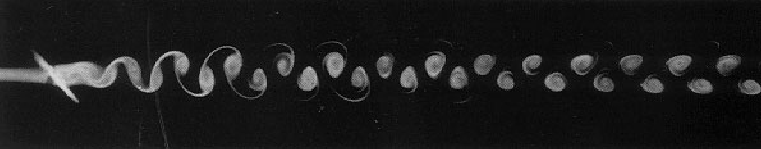
\includegraphics[width=\textwidth]{images/10/vortices.png}
    \caption{Scia di Von Karman}
\end{figure}

\noindent Il vortex shedding è una fenomenologia non stazionaria che si genera non solo attorno al cilindro ma anche a valle di altri corpi tozzi bidimensionali e tridimensionali. Per esempio, nella scia degli autoveicoli è presente la traccia dello sfilamento di vortici che si originano prevalentemente dalla parte posteriore del corpo. Anche nel caso di profili alari bidimensionali a elevata incidenza il fenomeno del vortex shedding si genera in modo molto evidente.\\\\
Il fenomeno è regolato da due parametri adimensionali: il numero di Reynolds ed il numero di Strouhal:
\begin{equation*}
    Re = \frac{U_\infty d}{\nu} \qquad St = \frac{f_s d}{U_\infty}
\end{equation*}
Alcune leggi empiriche che legano il numero di Strouhal al numero di Reynolds sono le seguenti:
\begin{equation*}
    \begin{dcases}
        St = 0.212\left(1-\frac{21.2}{Re}\right) \quad &\text{Per } 50<Re\le150\\
        St = 0.212\left(1-\frac{17}{Re}\right) \quad &\text{Per } 150<Re\le300\\
        St = 0.212\left(1-\frac{12.7}{Re}\right) \quad &\text{Per } 300<Re\le2000
    \end{dcases}
\end{equation*}

\subsection{Catena di misura}
Per lo studio è stata utilizzata una sonda a filo caldo posizionata in prossimità della mezzeria di un filo di acciaio armonico del diametro $d=1$ mm teso da parete a parete della camera di prova di una galleria del vento aperta.
\begin{figure}[H]
    \centering
    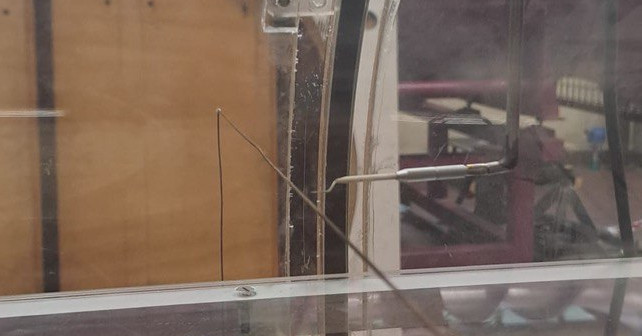
\includegraphics[width=.7\textwidth]{images/10/filo.jpg}
    \caption{Filo di acciaio armonico con sonda a filo caldo opportunamente posizionata}
\end{figure}

\noindent Per misurare la velocità del flusso in galleria del vento, si utilizza un tubo di Pitot collegato al trasduttore di pressione Setra 239 C.\\\\
La catena di misura è quindi composta da:
\begin{itemize}
    \item Galleria del vento aperta;
    \item Filo di acciaio (cilindro) di diametro 1 mm;
    \item Tubo di Pitot;
    \item Trasduttore di pressione Setra 239 C;
    \item Sonda a filo caldo Dantec P15;
    \item Sistema di acquisizione dati e PC con LabView.
\end{itemize}

\subsection{Procedura sperimentale}
Come primo passo si misurano la pressione e la temperatura ambiente, dalle quali si ricava la densità utilizzando la legge dei gas perfetti e la viscosità dinamica utilizzando la legge di Sutherland:
\begin{equation*}
    \rho = \frac{p_{amb}}{RT_{amb}} \qquad \mu = 1.46\cdot10^{-6} \frac{T_{amb}^{3/2}}{T_{amb}+110} 
\end{equation*}
Successivamente è necessario bilanciare il ponte di Wheatstone della sonda. A galleria spenta, la tensione di bilanciamento deve essere tale da avere una differenza di potenziale nulla ai capi della sonda a filo caldo.\\\\
Per ogni velocità $U$ del flusso in galleria del vento, una volta esauriti eventuali fenomeni transitori, sono effettuate due letture: una relativa al segnale di tensione in uscita dal trasduttore di pressione collegato al tubo di Pitot $E_t$, necessario per calcolare la velocità del flusso, ed un'altra relativa alla frequenza di shedding misurata dalla sonda a filo caldo.\\\\
Per misurare la frequenza di shedding, occorre campionare con una certa frequenza di campionamento $f_{samp}$ il segnale di tensione in uscita dalla sonda a filo caldo per un periodo di tempo $T$. Una volta ottenuto il segnale $E_{HW}(t)$ nel periodo di tempo $T$, si ricava lo spettro di potenza mediante il metodo di Welch. Questa operazione è automatizzata dal software di acquisizione ed elaborazione dati LabView. Dal diagramma dello spettro di potenza è possibile ricavare la frequenza di shedding $f_s$, questa si presenta come la più piccola frequenza relativa ad un evidente picco nello spettro di potenza.\\\\
Bisogna fare attenzione ad utilizzare una frequenza di campionamento adeguata, infatti, secondo il teorema di Nyquist, la massima risoluzione nel dominio delle frequenze è pari alla metà della frequenza di campionamento, pertanto la frequenza di campionamento deve essere almeno il doppio della frequenza di shedding, altrimenti questa non potrà essere rilevata.
\begin{figure}[H]
    \centering
    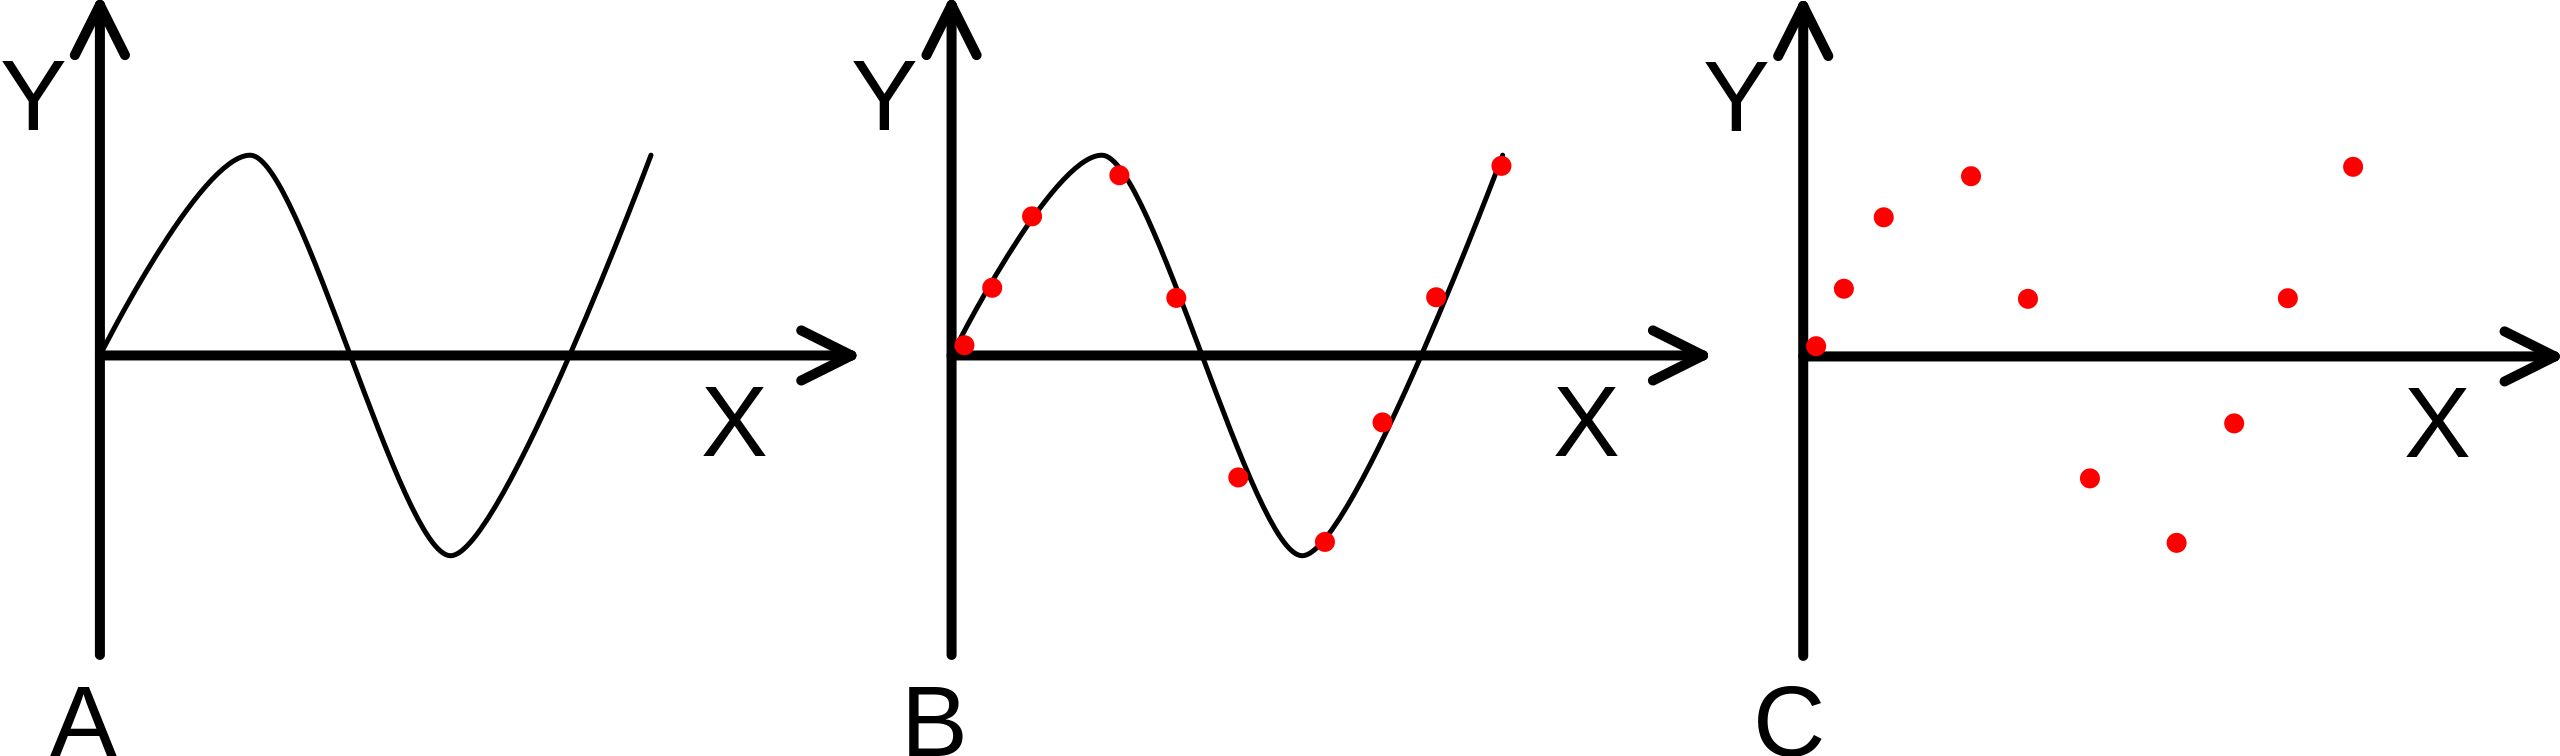
\includegraphics[width=.7\textwidth]{images/10/nyquist.png}
    \caption{Segnale analogico, segnale analogico campionato e campioni da quantizzare}
\end{figure}

\noindent I dati grezzi misurati con la procedura appena descritta sono riportati nelle tabelle in appendice \ref{a10}.

\subsection{Analisi dati}
L'analisi dati per la presente attività è condotta con l'ausilio di un codice Python, riportato in appendice \ref{b10}.\\\\
Come prima operazione è necessario misurare la tensione di offset del trasduttore di pressione Setra 239 C. Tale tensione per la presente indagine risulta essere pari a circa $E_{0t}=0.04$ V.\\\\
Utilizzando la costante di taratura del trasduttore di pressione precedentemente ricavata:
\begin{equation*}
    K_t =\ 550 \text{Pa/m}
\end{equation*}
Si misura la pressione dinamica e quindi la velocità del flusso rilevata dal tubo di Pitot:
\begin{equation*}
    U_{\infty} = \sqrt{\frac{2K_t(E_{t}-E_{0t})}\rho}
\end{equation*}
Si può quindi diagrammare l'andamento della frequenza di shedding in funzione della velocità a monte. Da come si vede nei seguenti diagrammi per le quattro squadre, questi rappresentano una disposizione rettilinea dei dati sperimentali:
\begin{figure}[H]
    \centering
    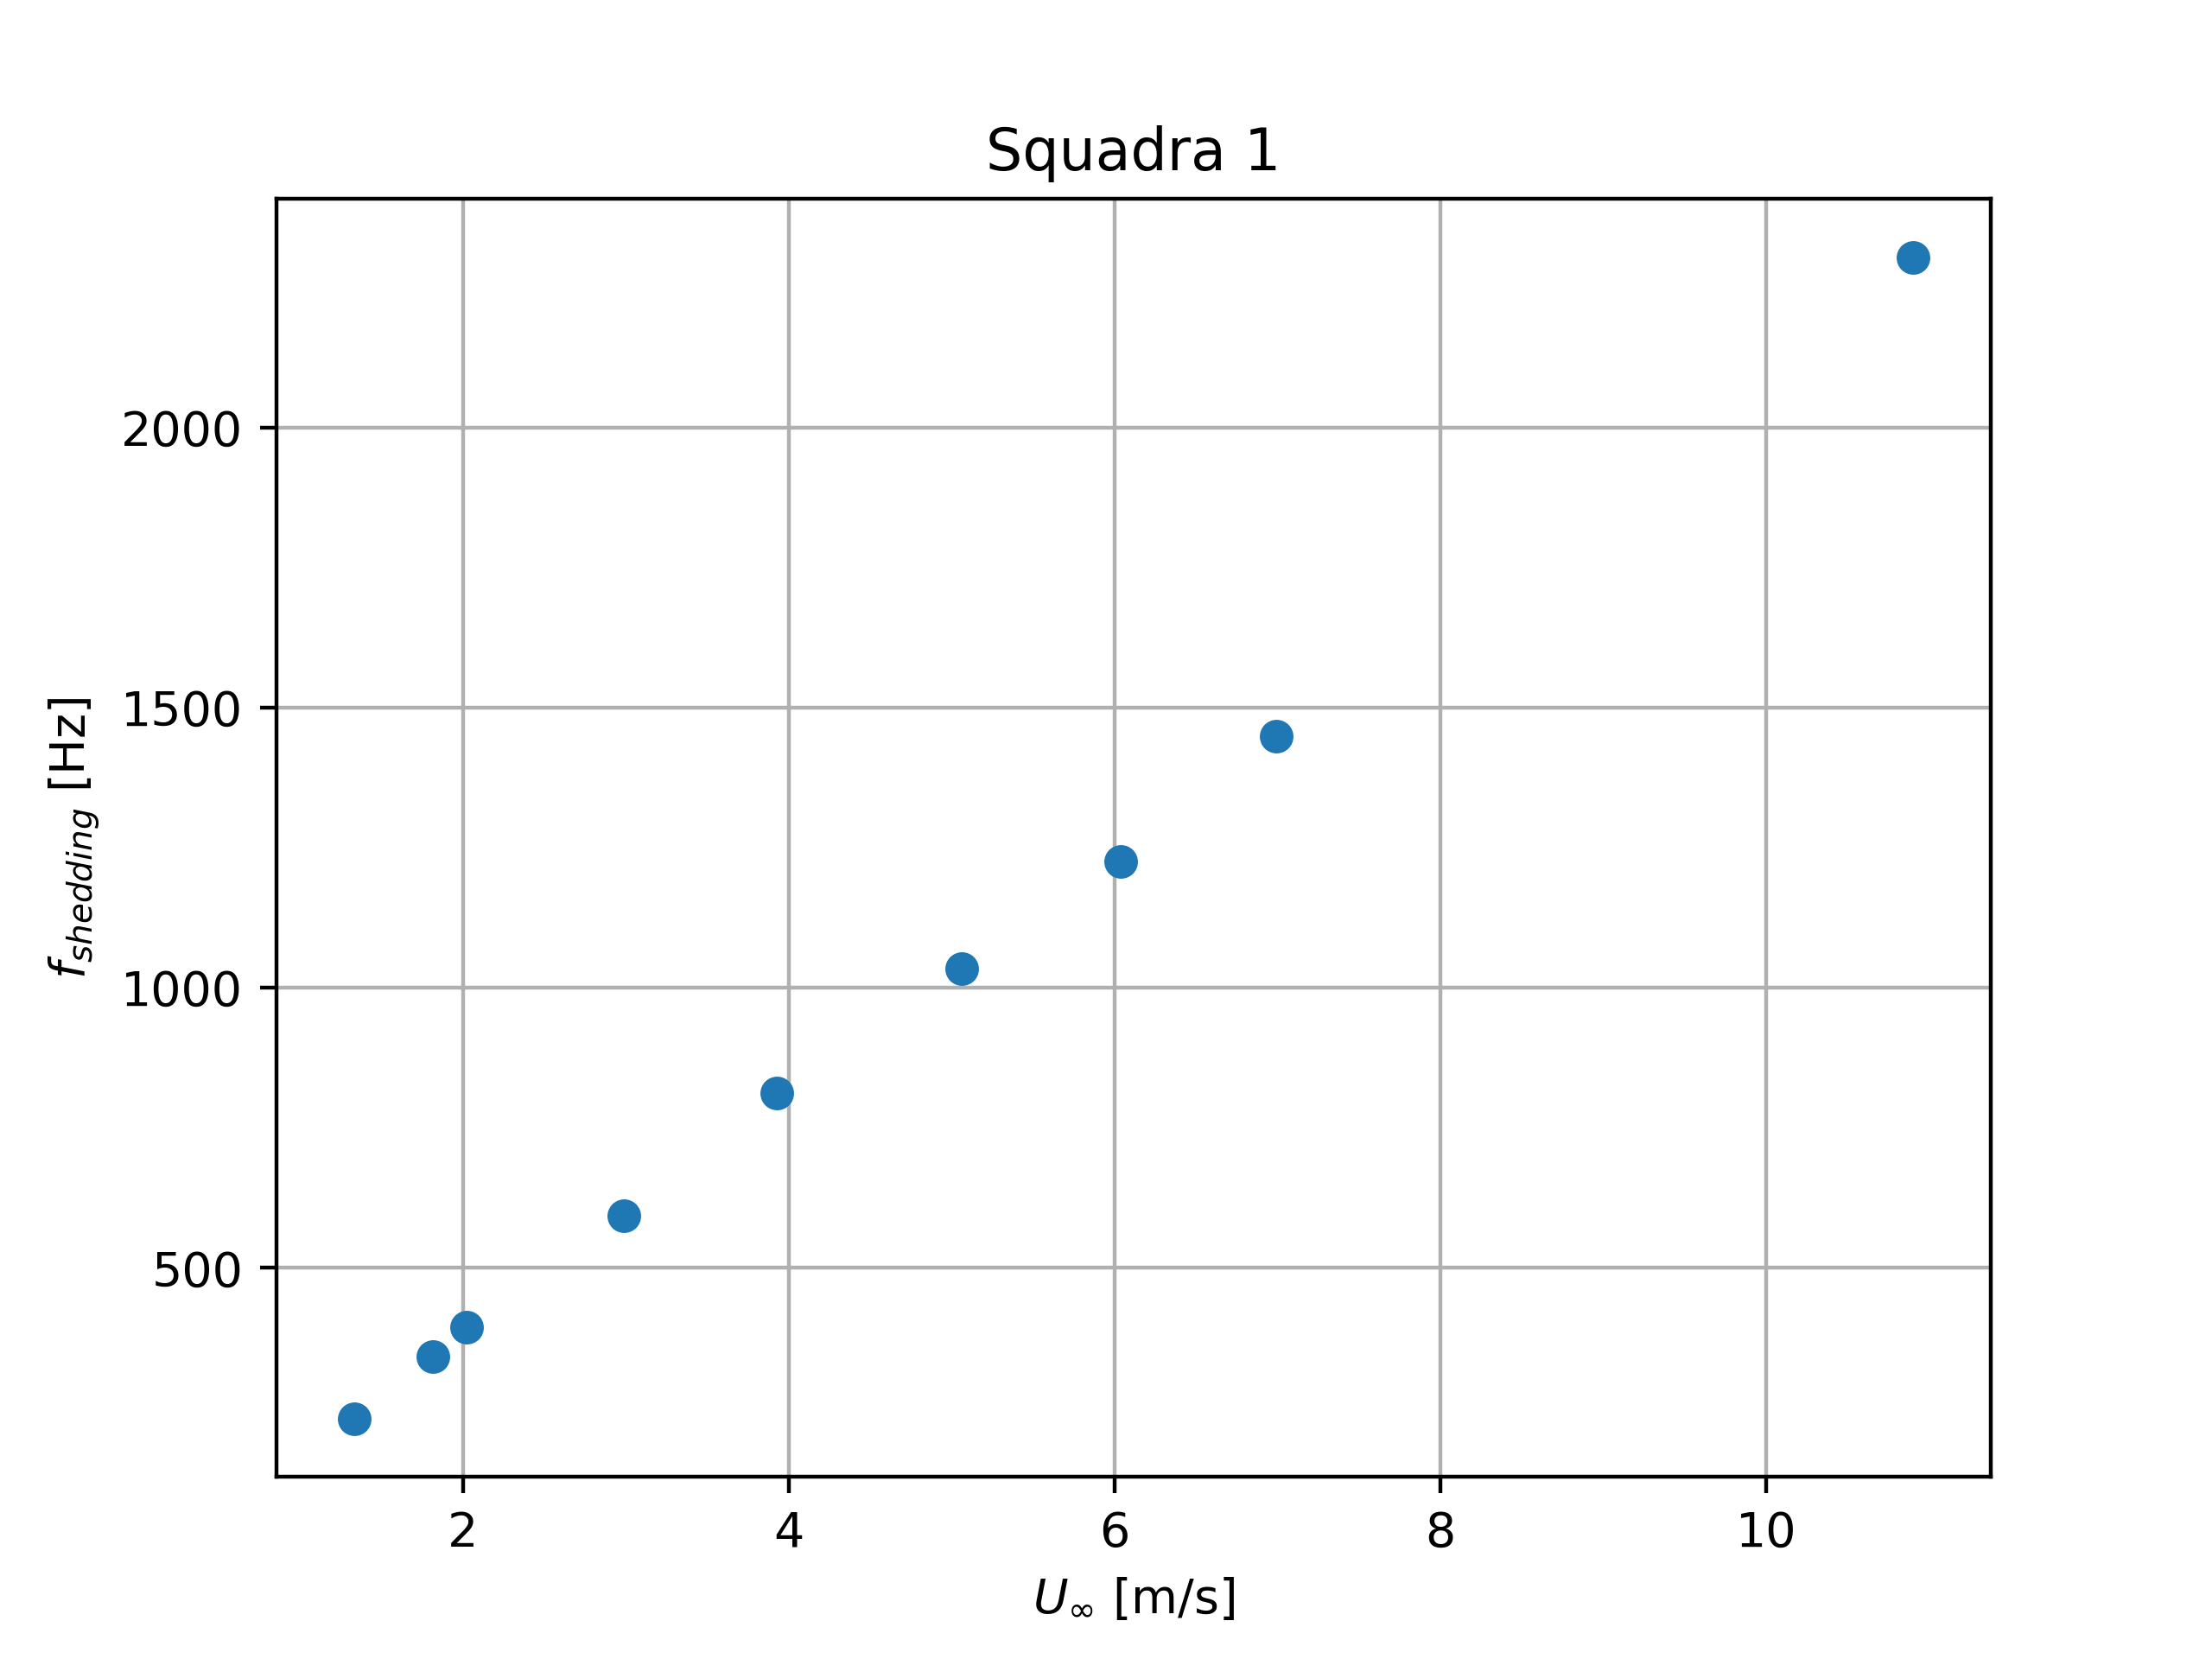
\includegraphics[width=.9\textwidth]{images/10/sq1.png}
    \caption{Diagramma $f_s(U_\infty)$ per la squadra 1}
\end{figure}
\begin{figure}[H]
    \centering
    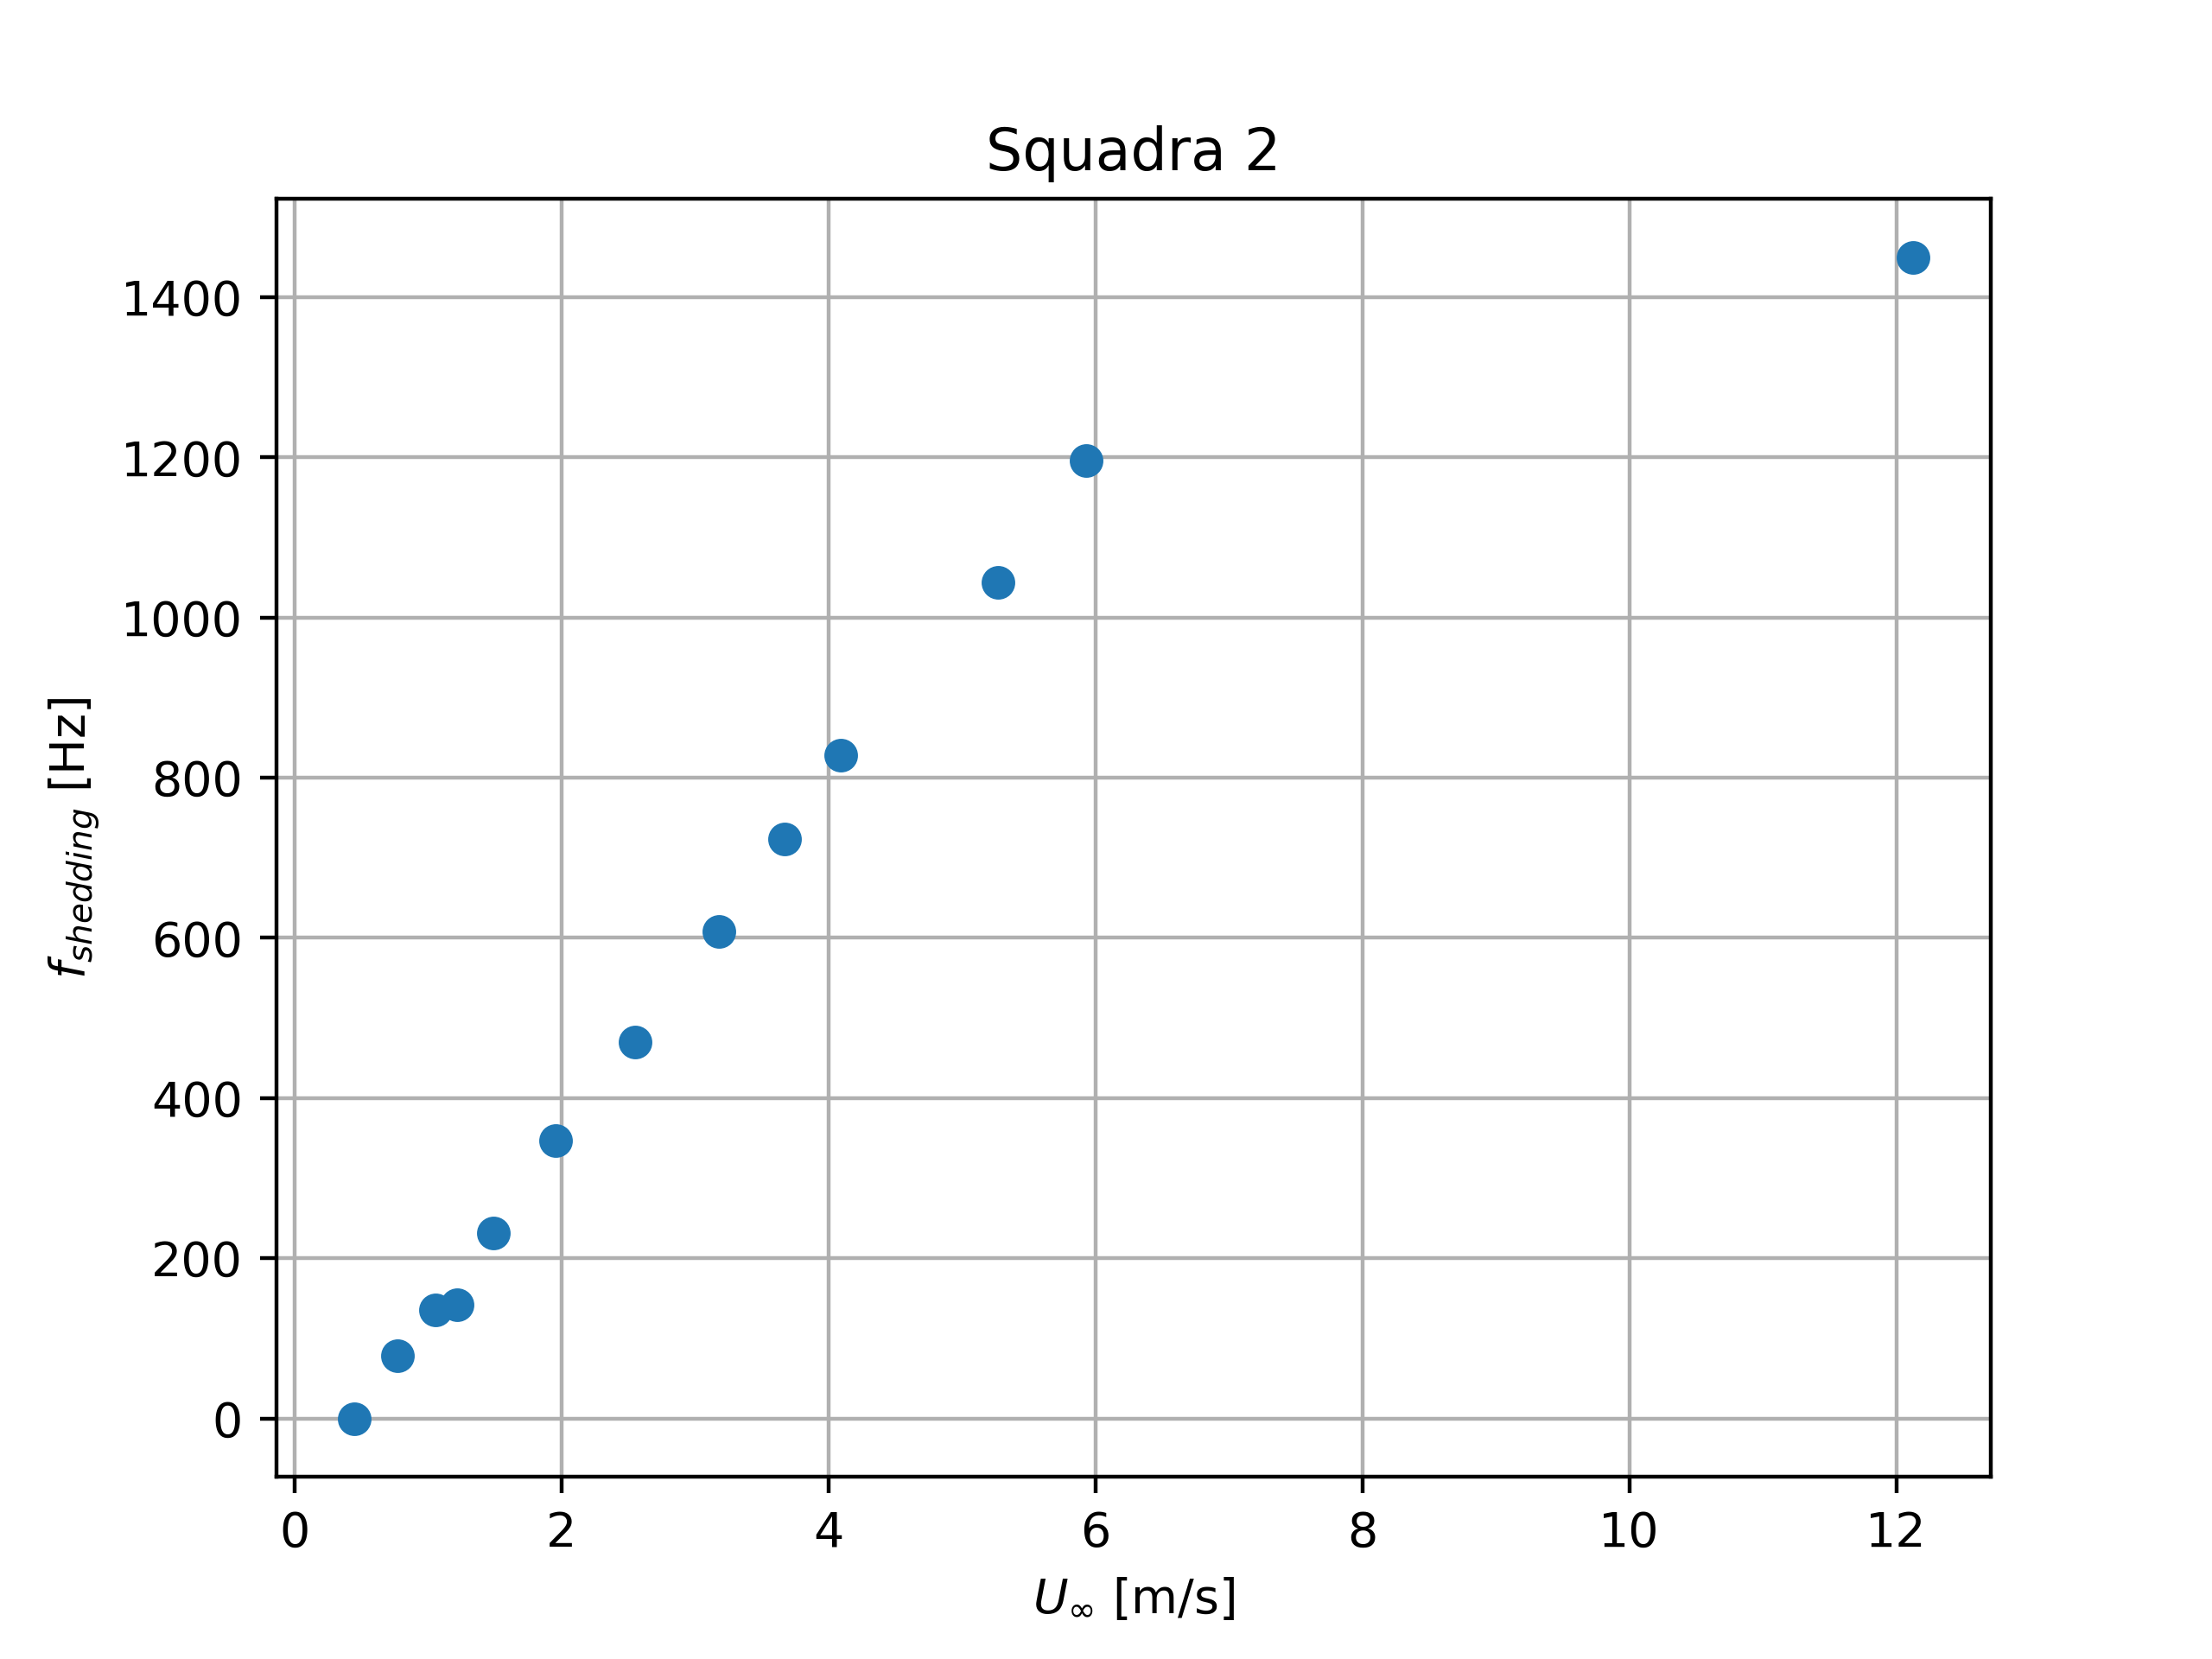
\includegraphics[width=.85\textwidth]{images/10/sq2.png}
    \caption{Diagramma $f_s(U_\infty)$ per la squadra 2}
\end{figure}
\begin{figure}[H]
    \centering
    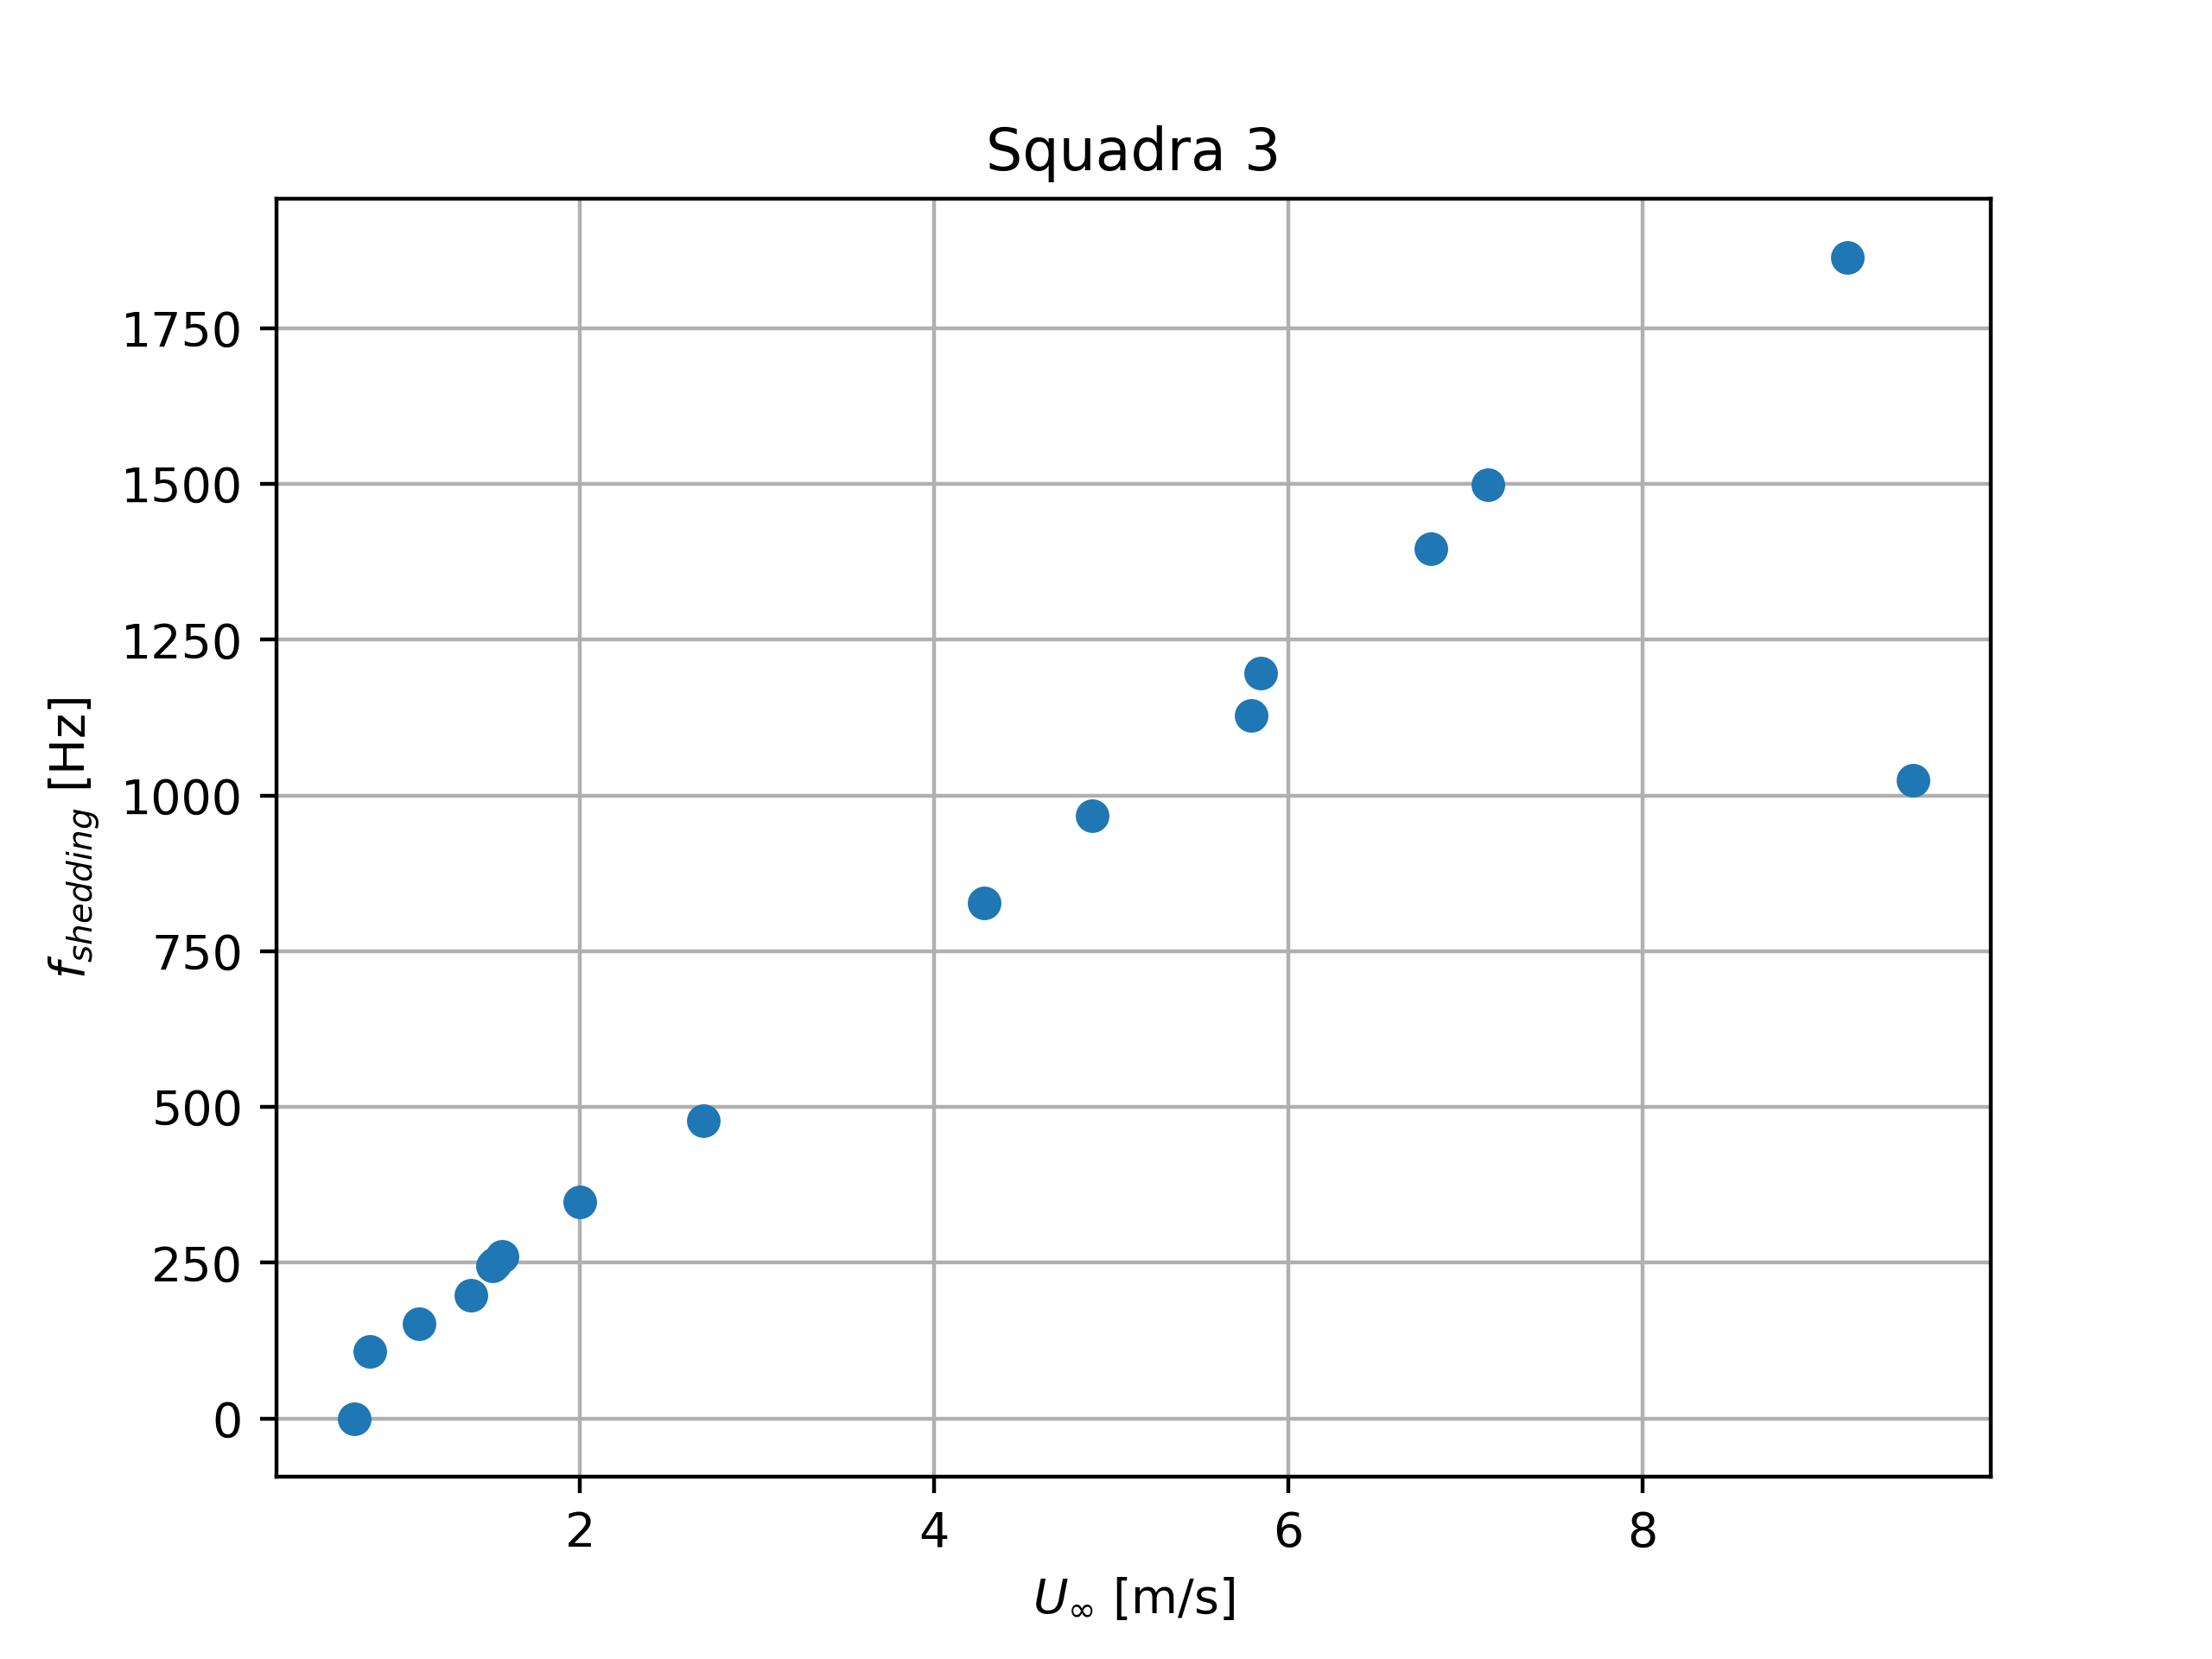
\includegraphics[width=.85\textwidth]{images/10/sq3.png}
    \caption{Diagramma $f_s(U_\infty)$ per la squadra 3}
\end{figure}
\begin{figure}[H]
    \centering
    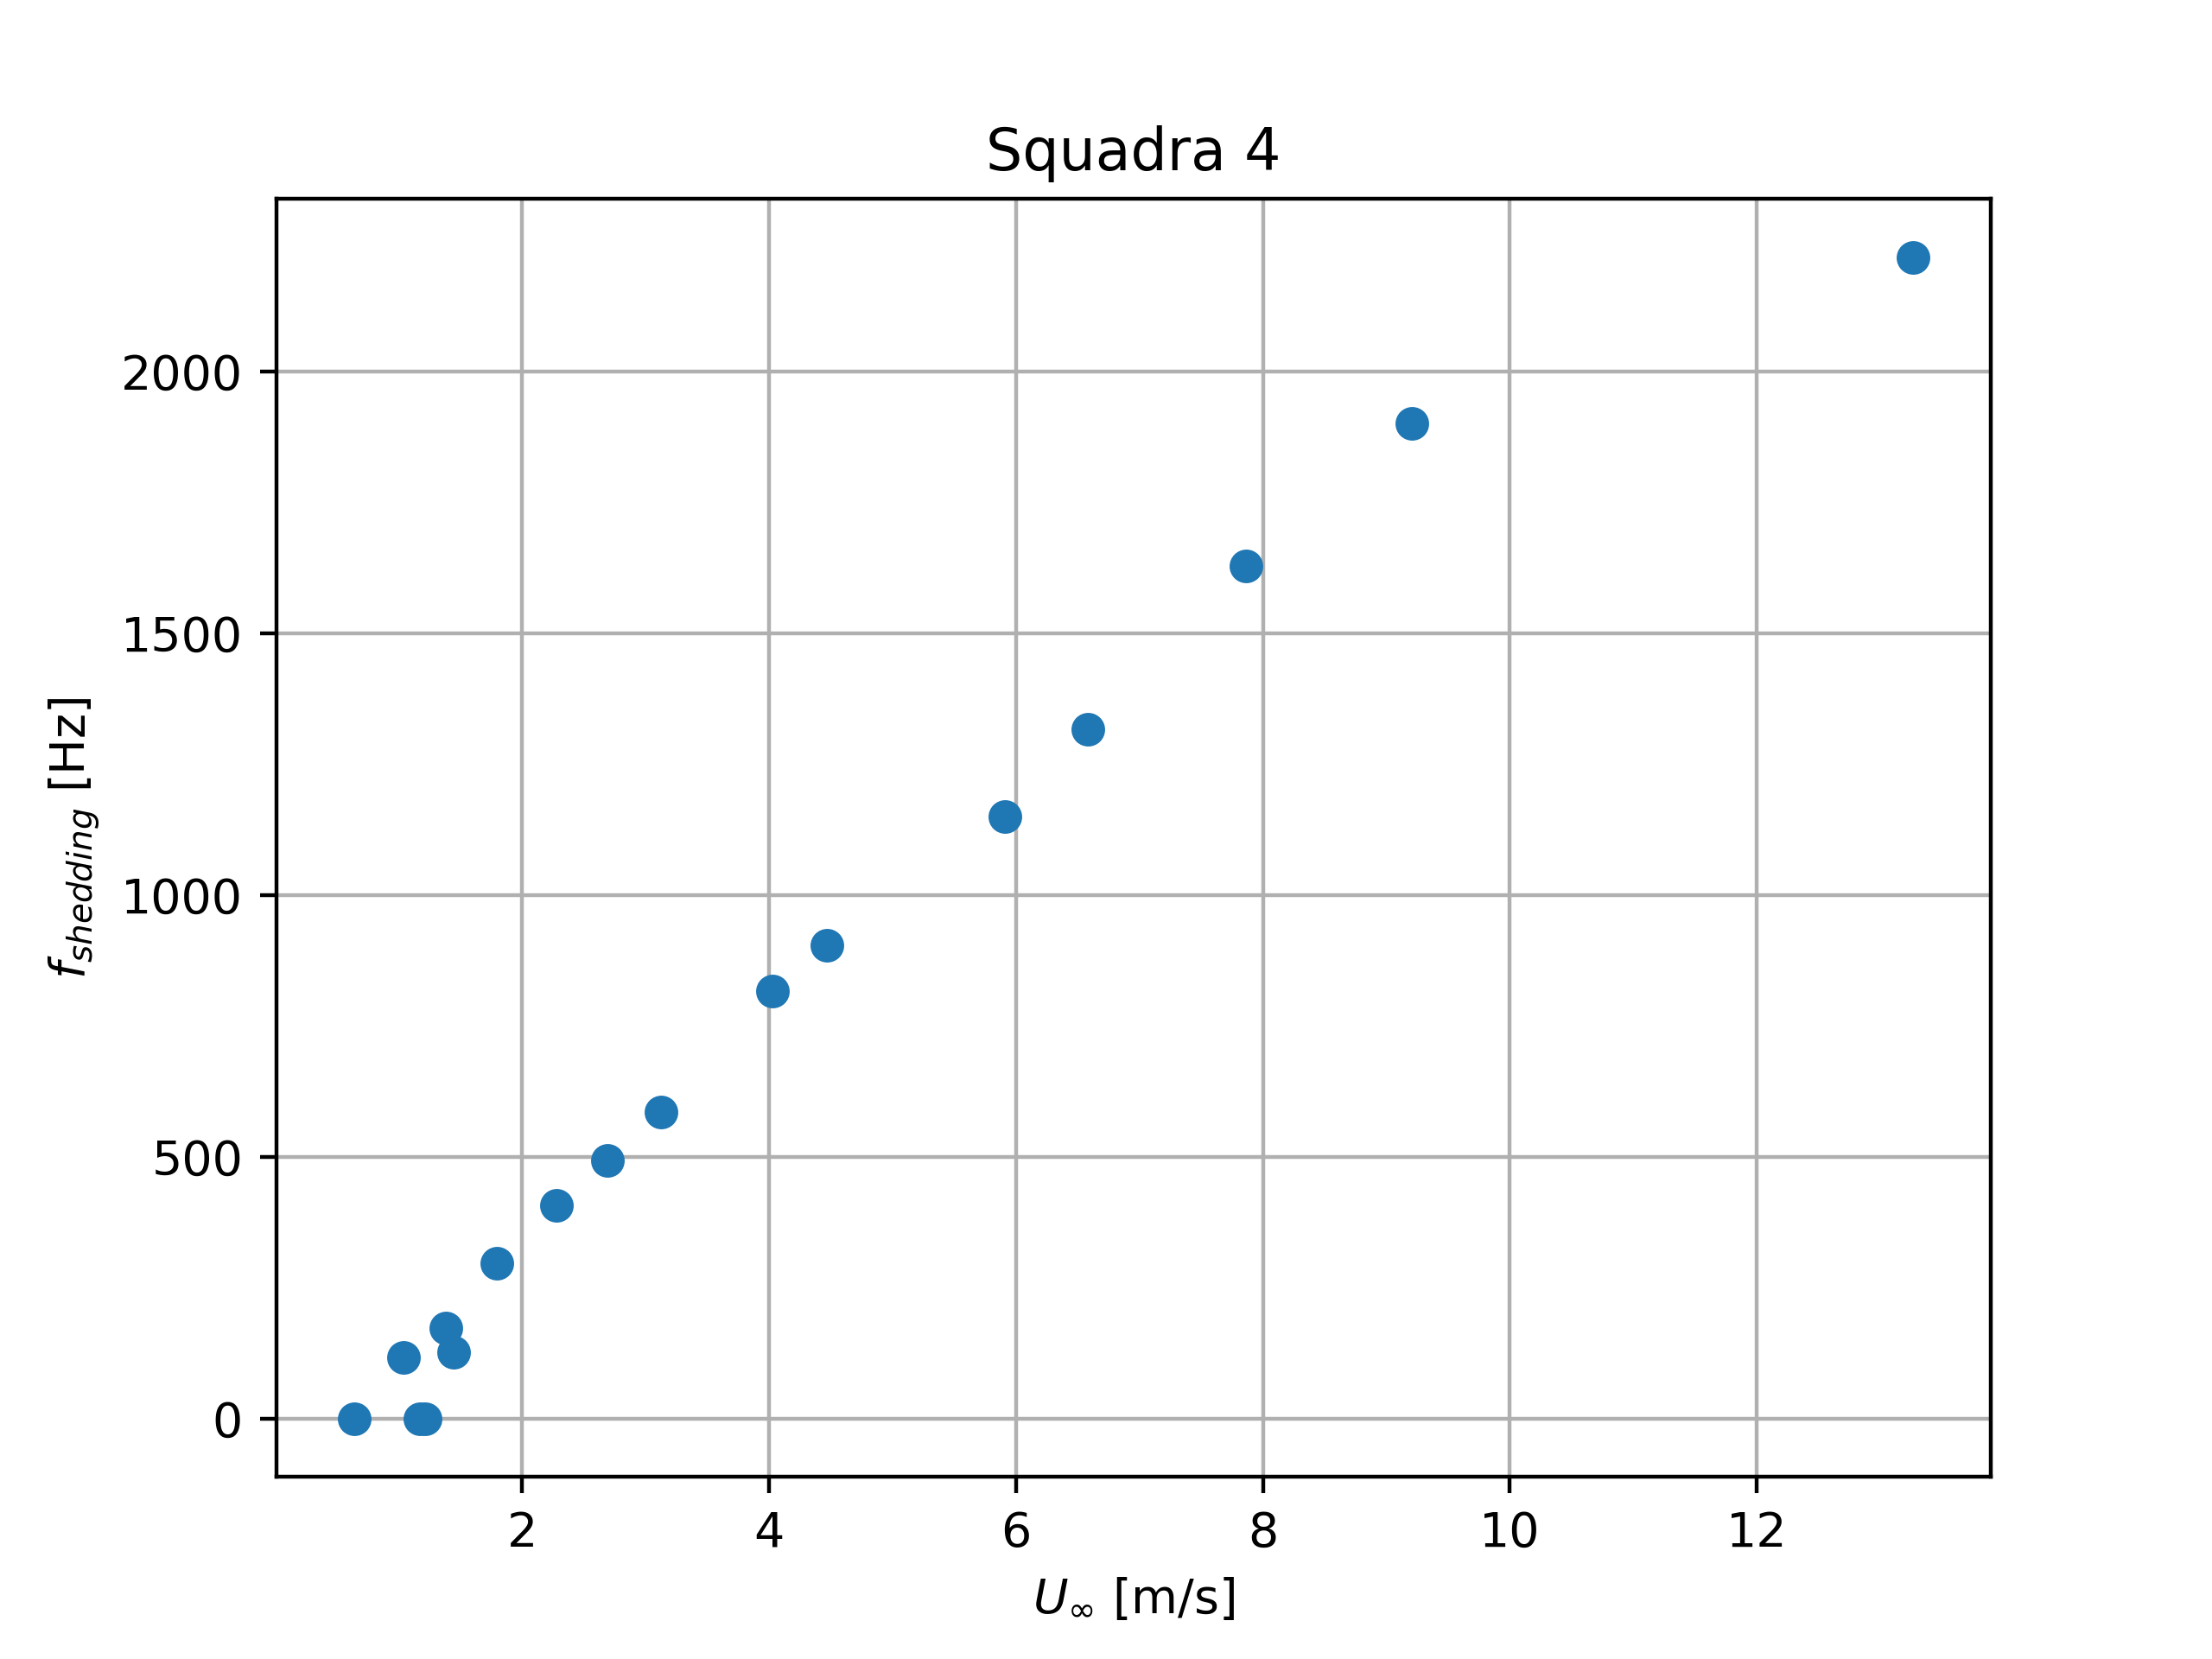
\includegraphics[width=.9\textwidth]{images/10/sq4.png}
    \caption{Diagramma $f_s(U_\infty)$ per la squadra 4}
\end{figure}

\noindent Alcuni dei punti sperimentali, in particolare per le squadre 2, 3 e 4, risultano essere sfasati rispetto all'andamento rettilineo. Questo potrebbe essere dovuto al teorema di Nyquist, tali frequenze di shedding non sono quindi state correttamente rilevate per via di una frequenza di campionamento troppo bassa.\\\\
Per passare ai parametri adimensionali, si calcolano il numero di Reynolds ed il numero di Strouhal:
\begin{equation*}
    Re = \frac{U_\infty d}{\nu} \qquad St = \frac{f_s d}{U_\infty}
\end{equation*}
Ricordando inoltre le leggi empiriche:
\begin{equation*}
    \begin{dcases}
        St = 0.212\left(1-\frac{21.2}{Re}\right) \quad &\text{Per } 50<Re\le150\\
        St = 0.212\left(1-\frac{17}{Re}\right) \quad &\text{Per } 150<Re\le300\\
        St = 0.212\left(1-\frac{12.7}{Re}\right) \quad &\text{Per } 300<Re\le2000
    \end{dcases}
\end{equation*}
Si ricavano i seguenti diagrammi per le quattro squadre:
\begin{figure}[H]
    \centering
    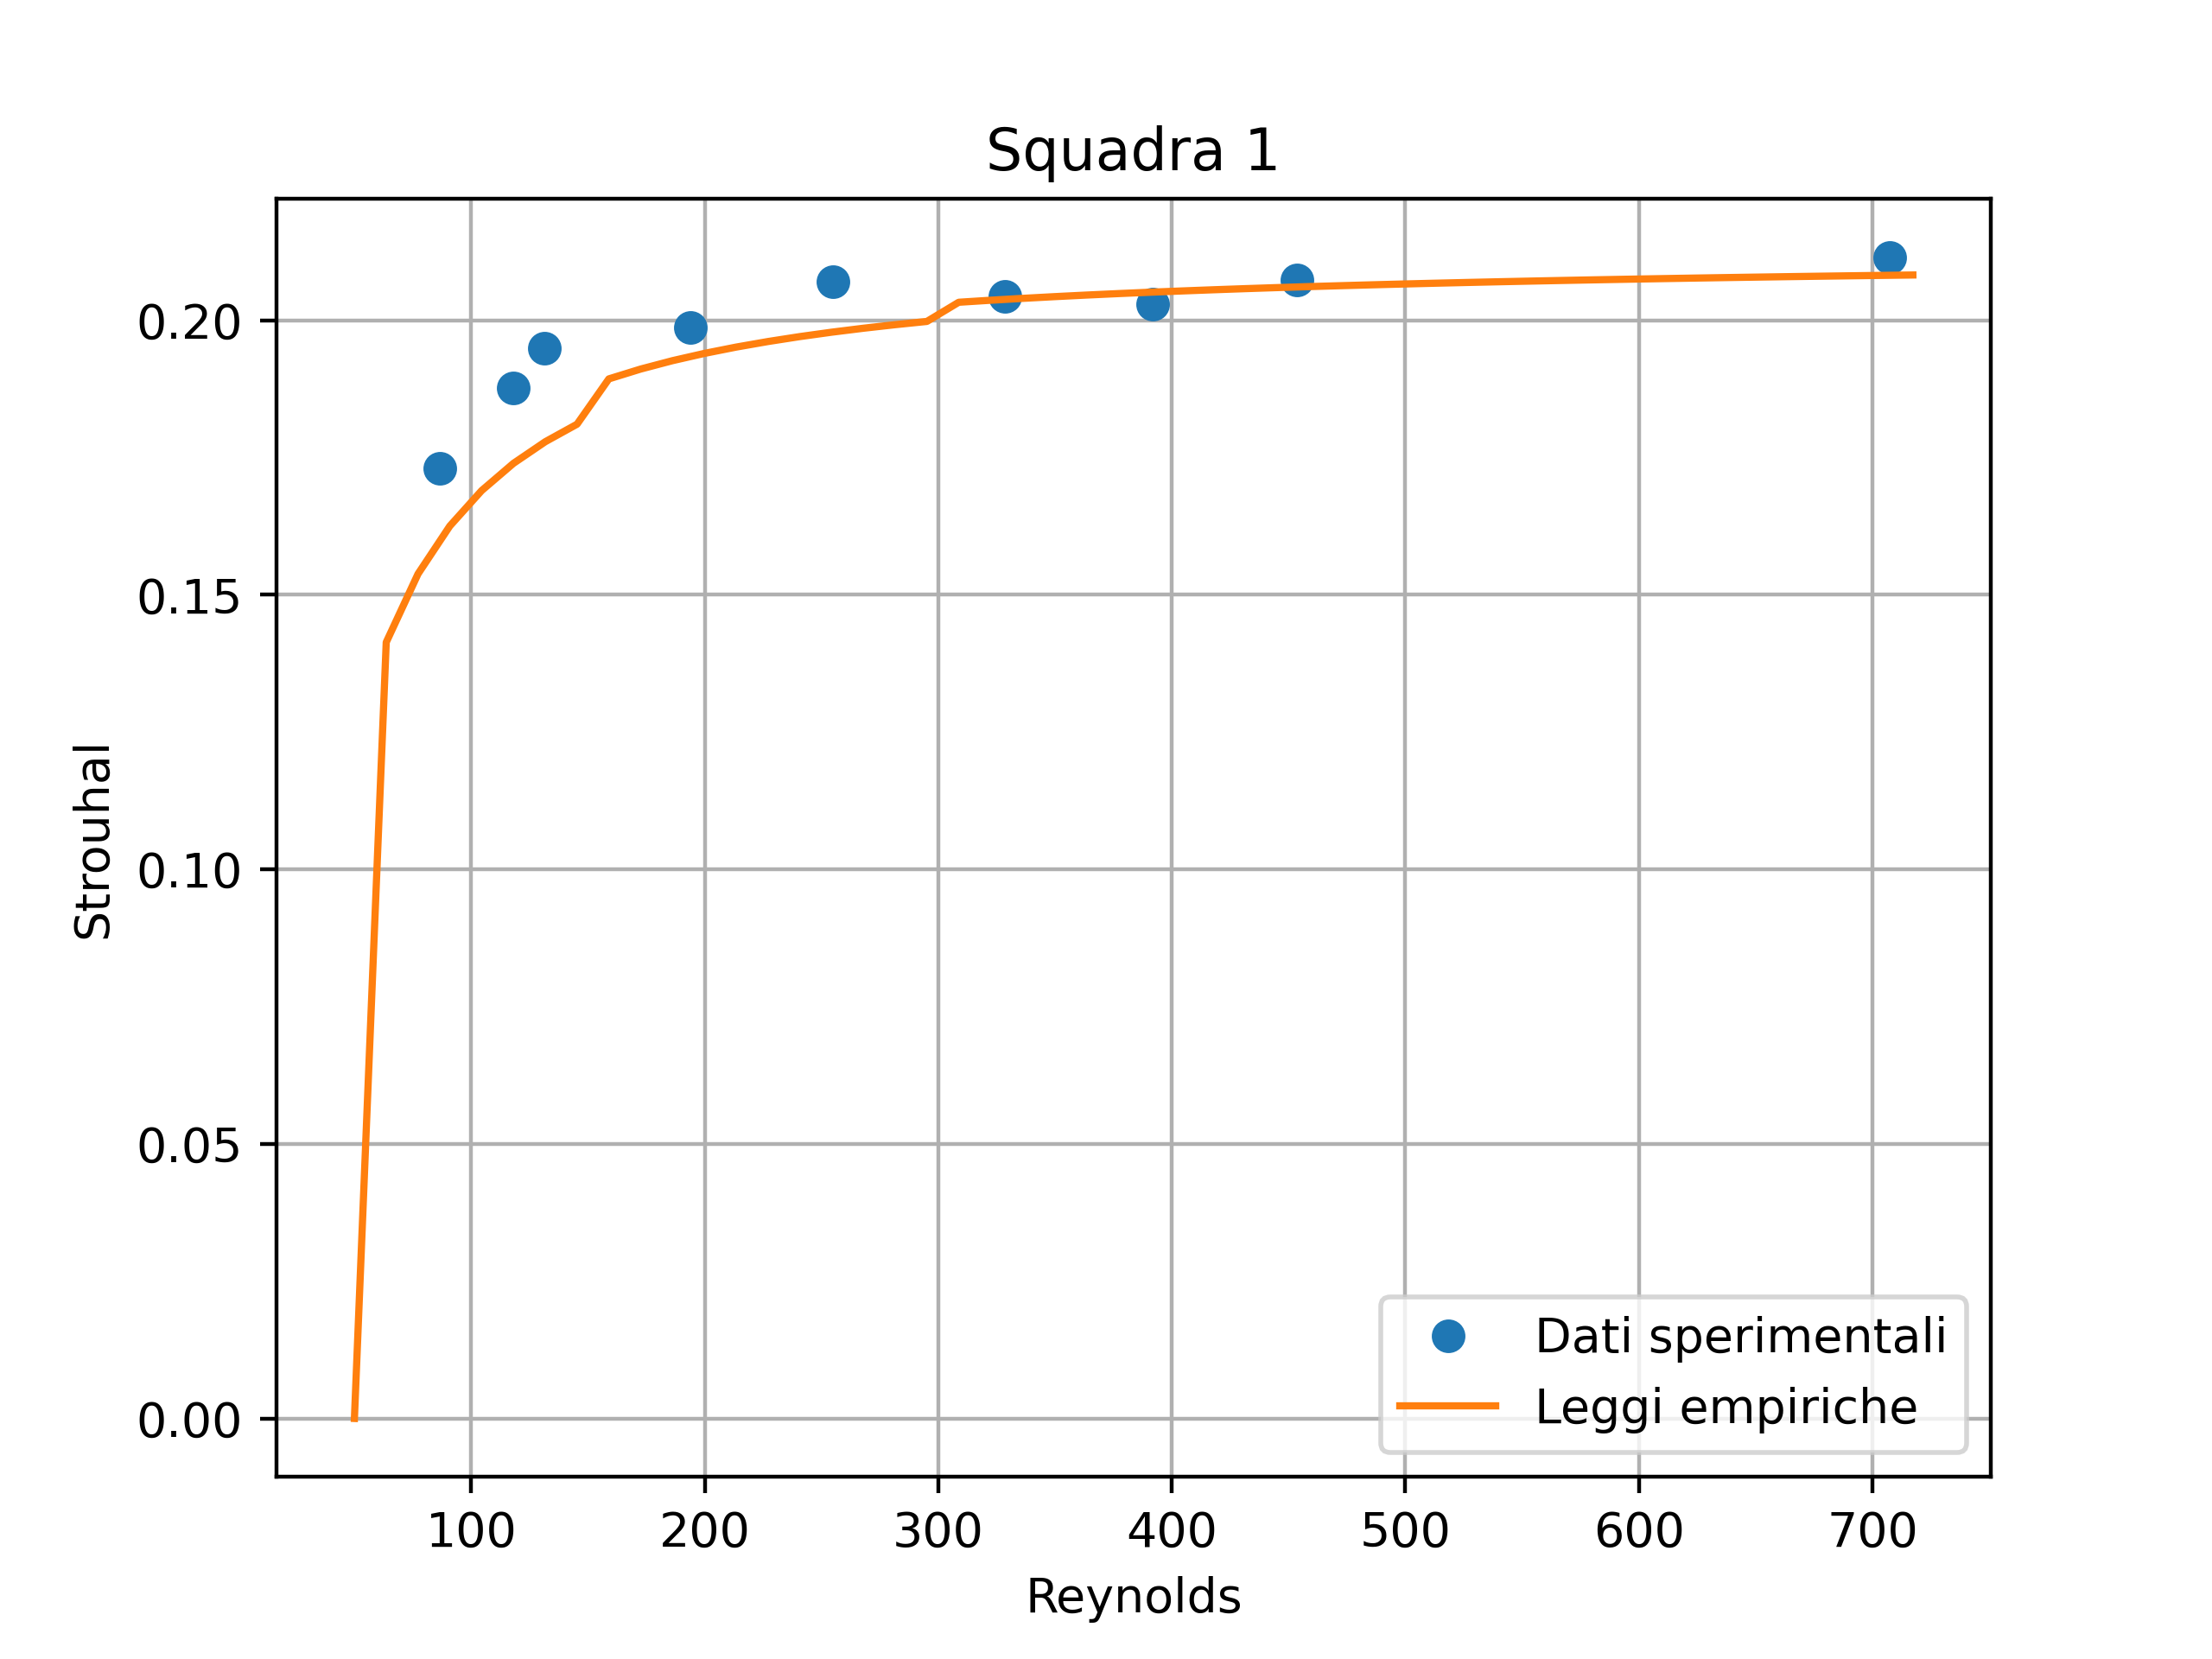
\includegraphics[width=.85\textwidth]{images/10/sq1adim.png}
    \caption{Diagramma $St(Re)$ per la squadra 1}
\end{figure}
\begin{figure}[H]
    \centering
    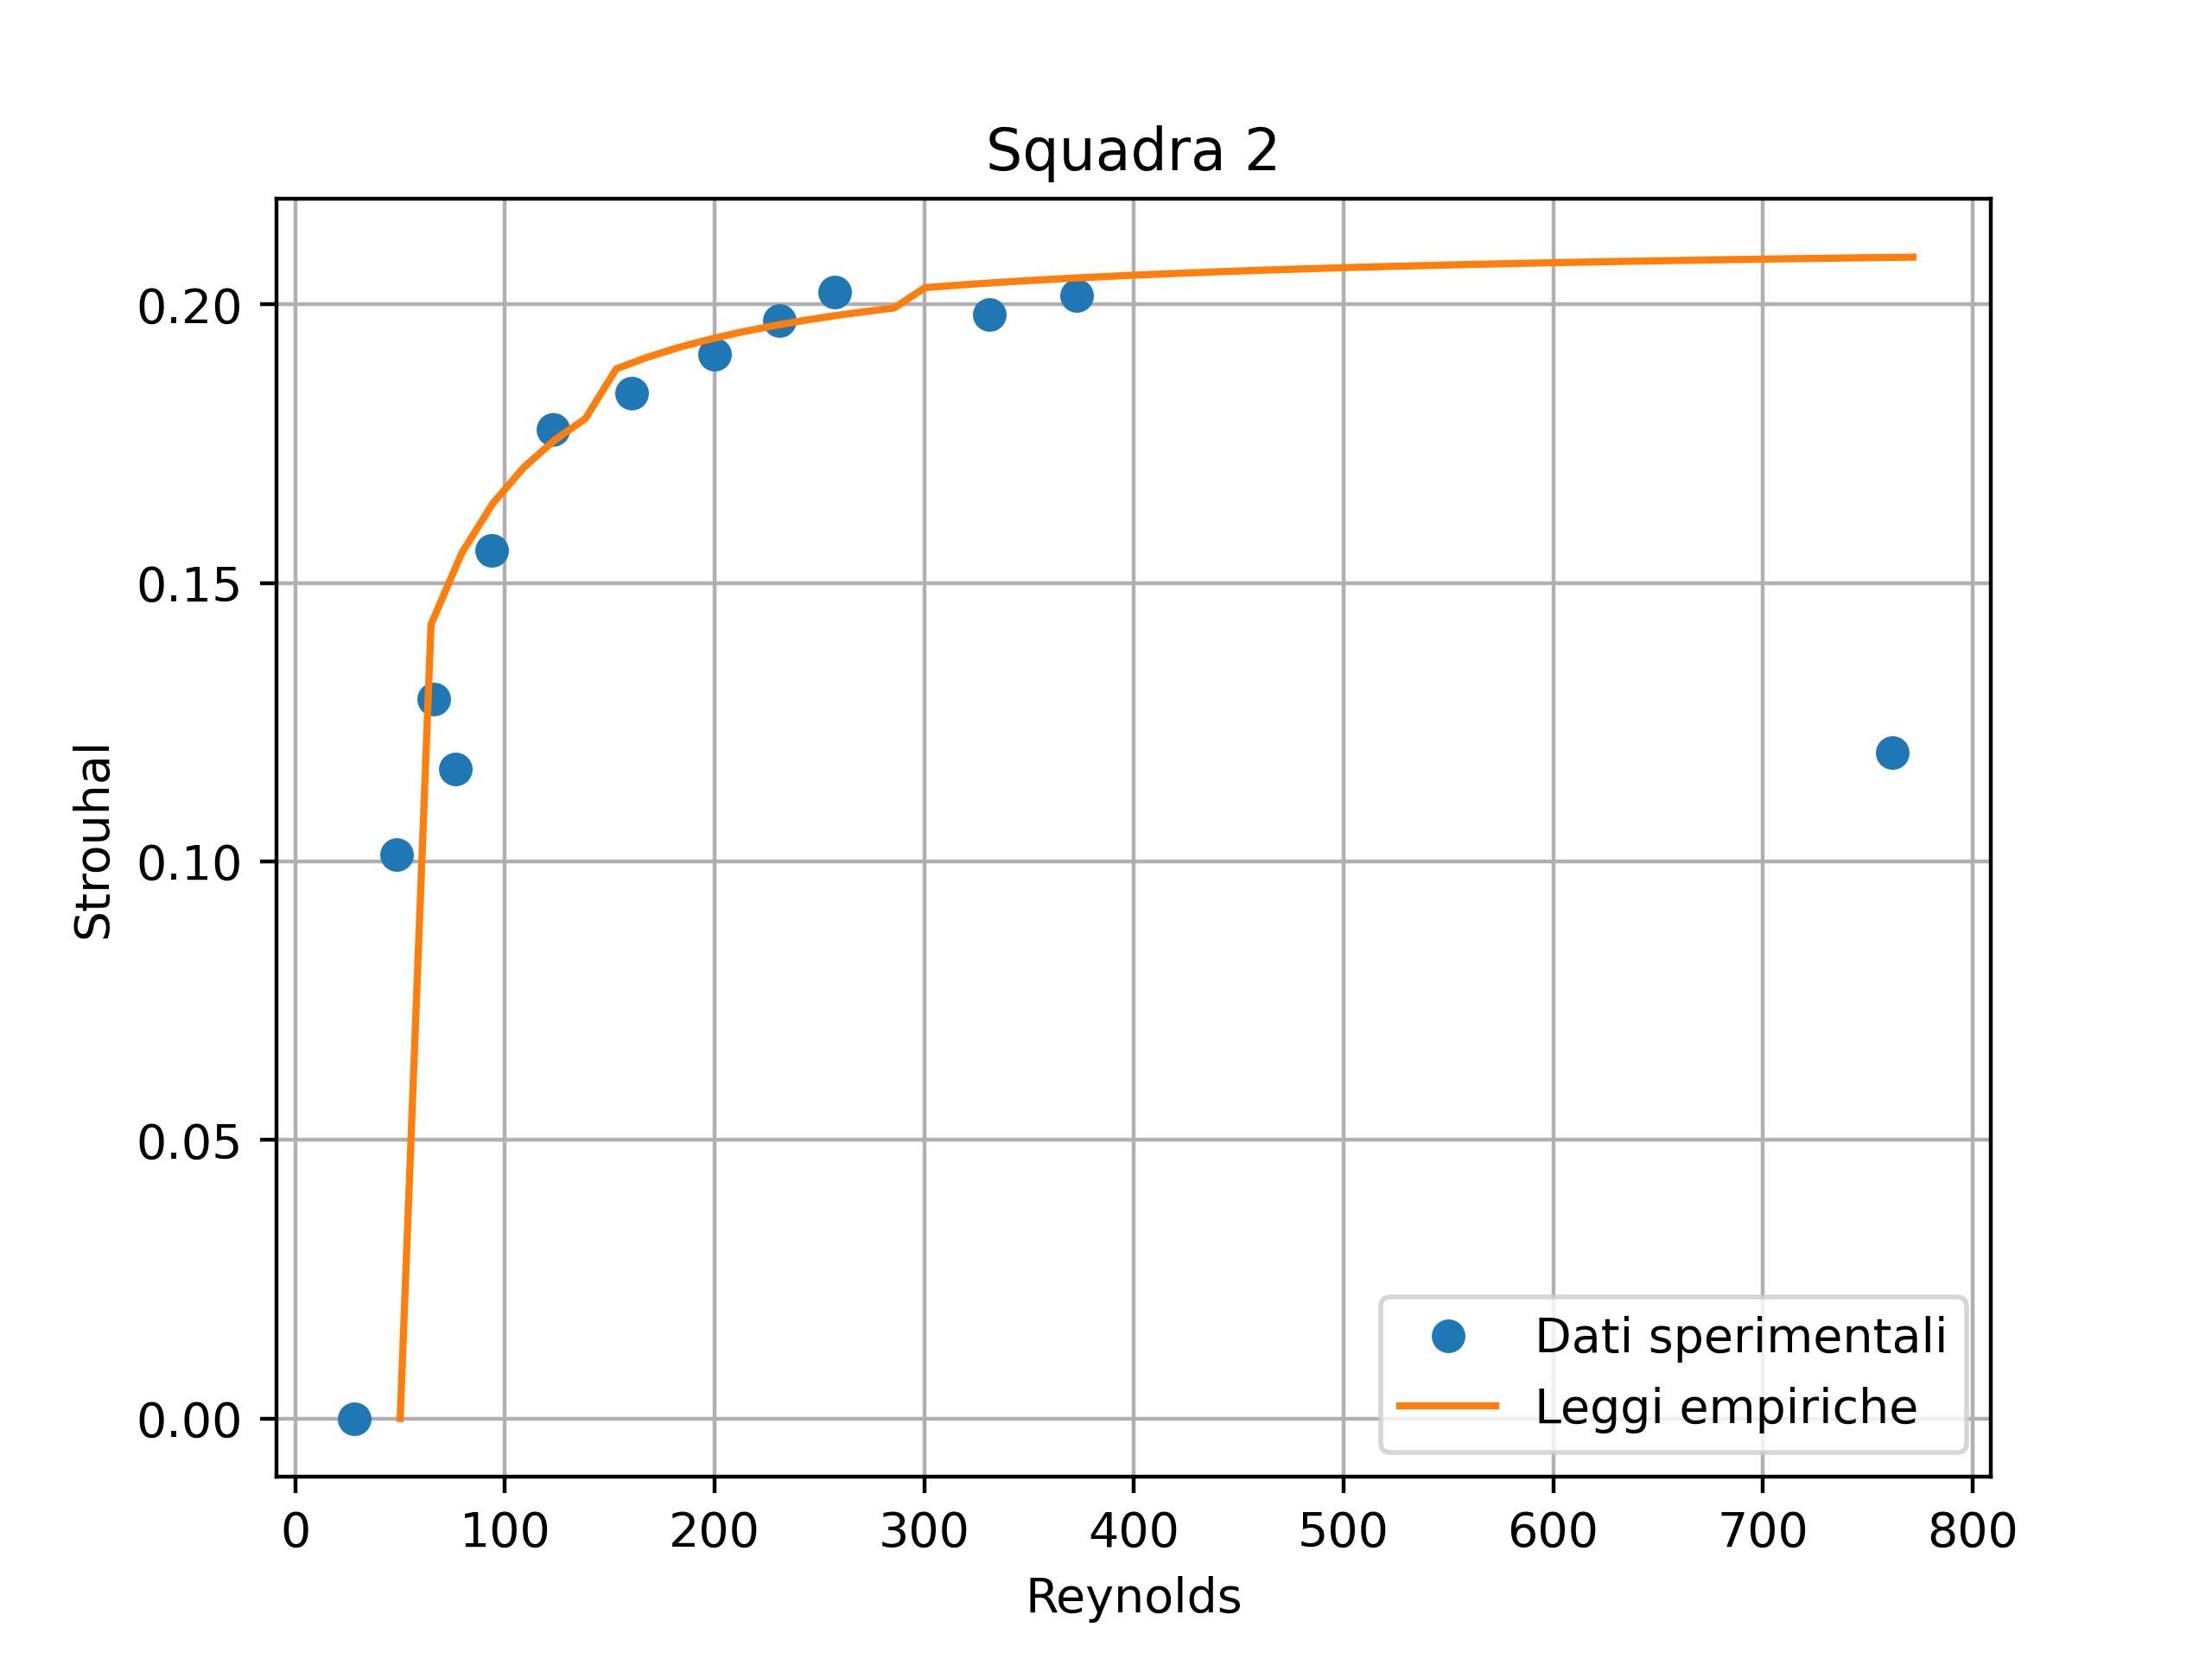
\includegraphics[width=.85\textwidth]{images/10/sq2adim.png}
    \caption{Diagramma $St(Re)$ per la squadra 2}
\end{figure}
\begin{figure}[H]
    \centering
    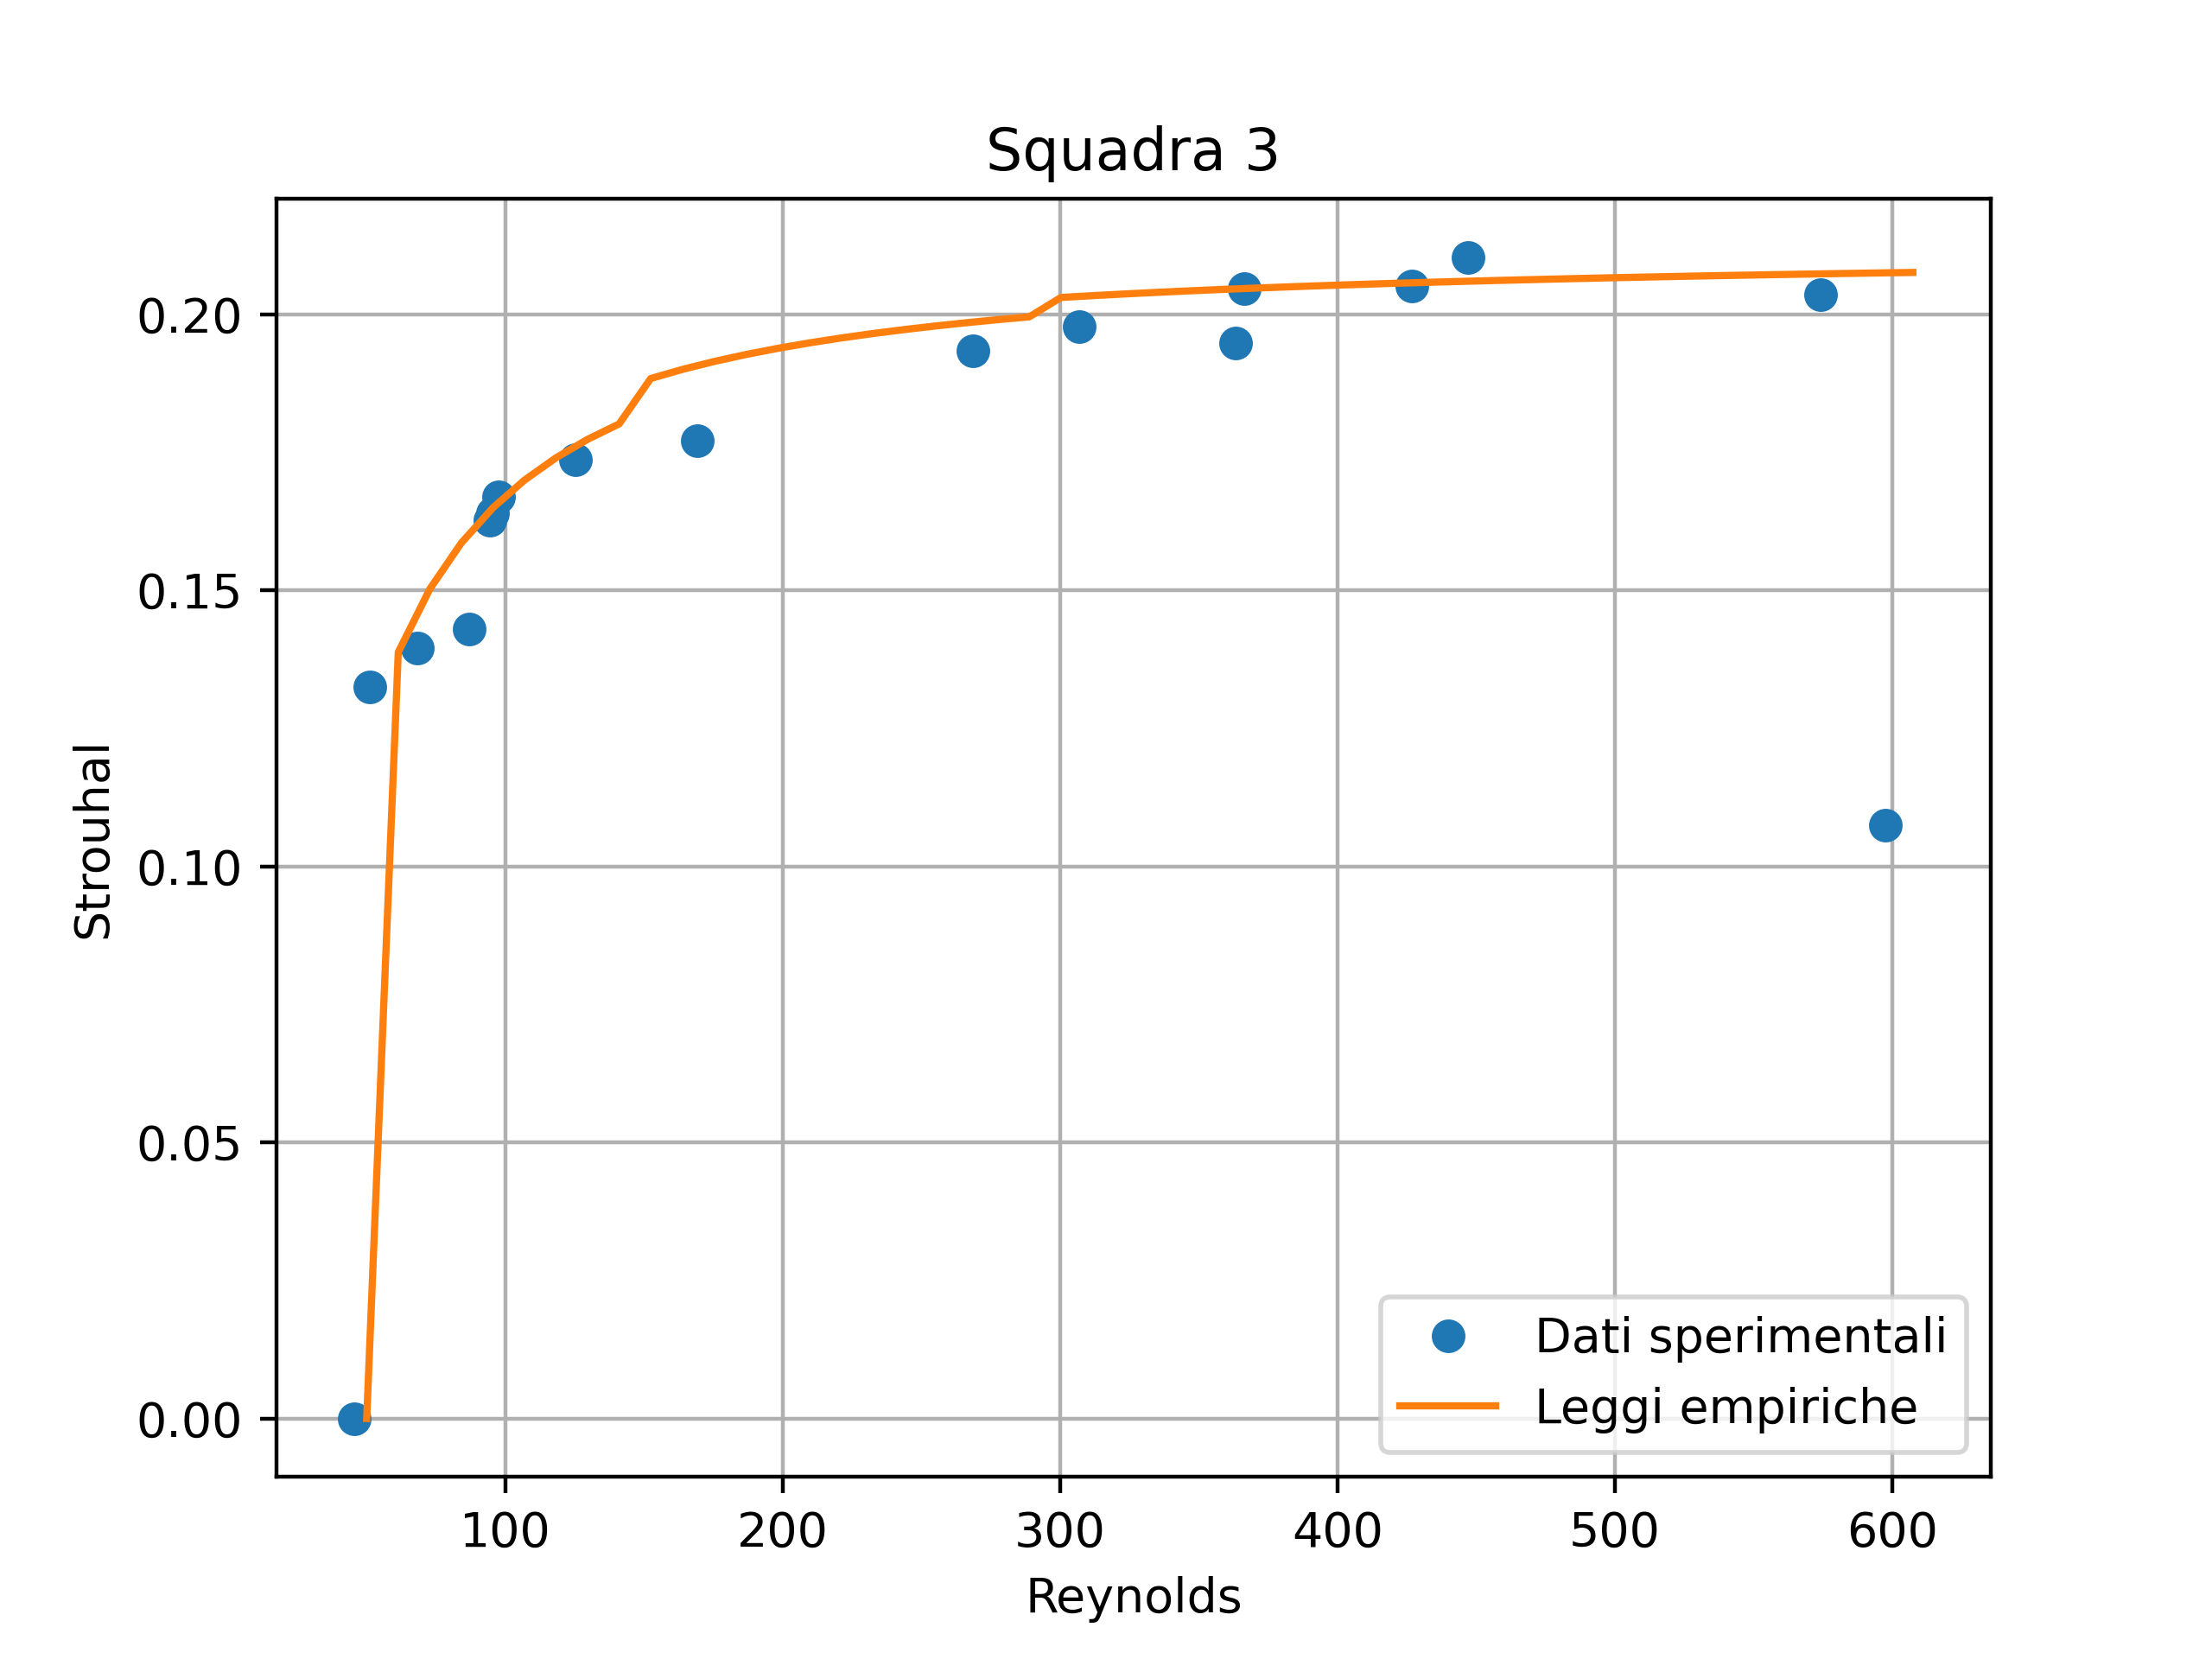
\includegraphics[width=.85\textwidth]{images/10/sq3adim.png}
    \caption{Diagramma $St(Re)$ per la squadra 3}
\end{figure}
\begin{figure}[H]
    \centering
    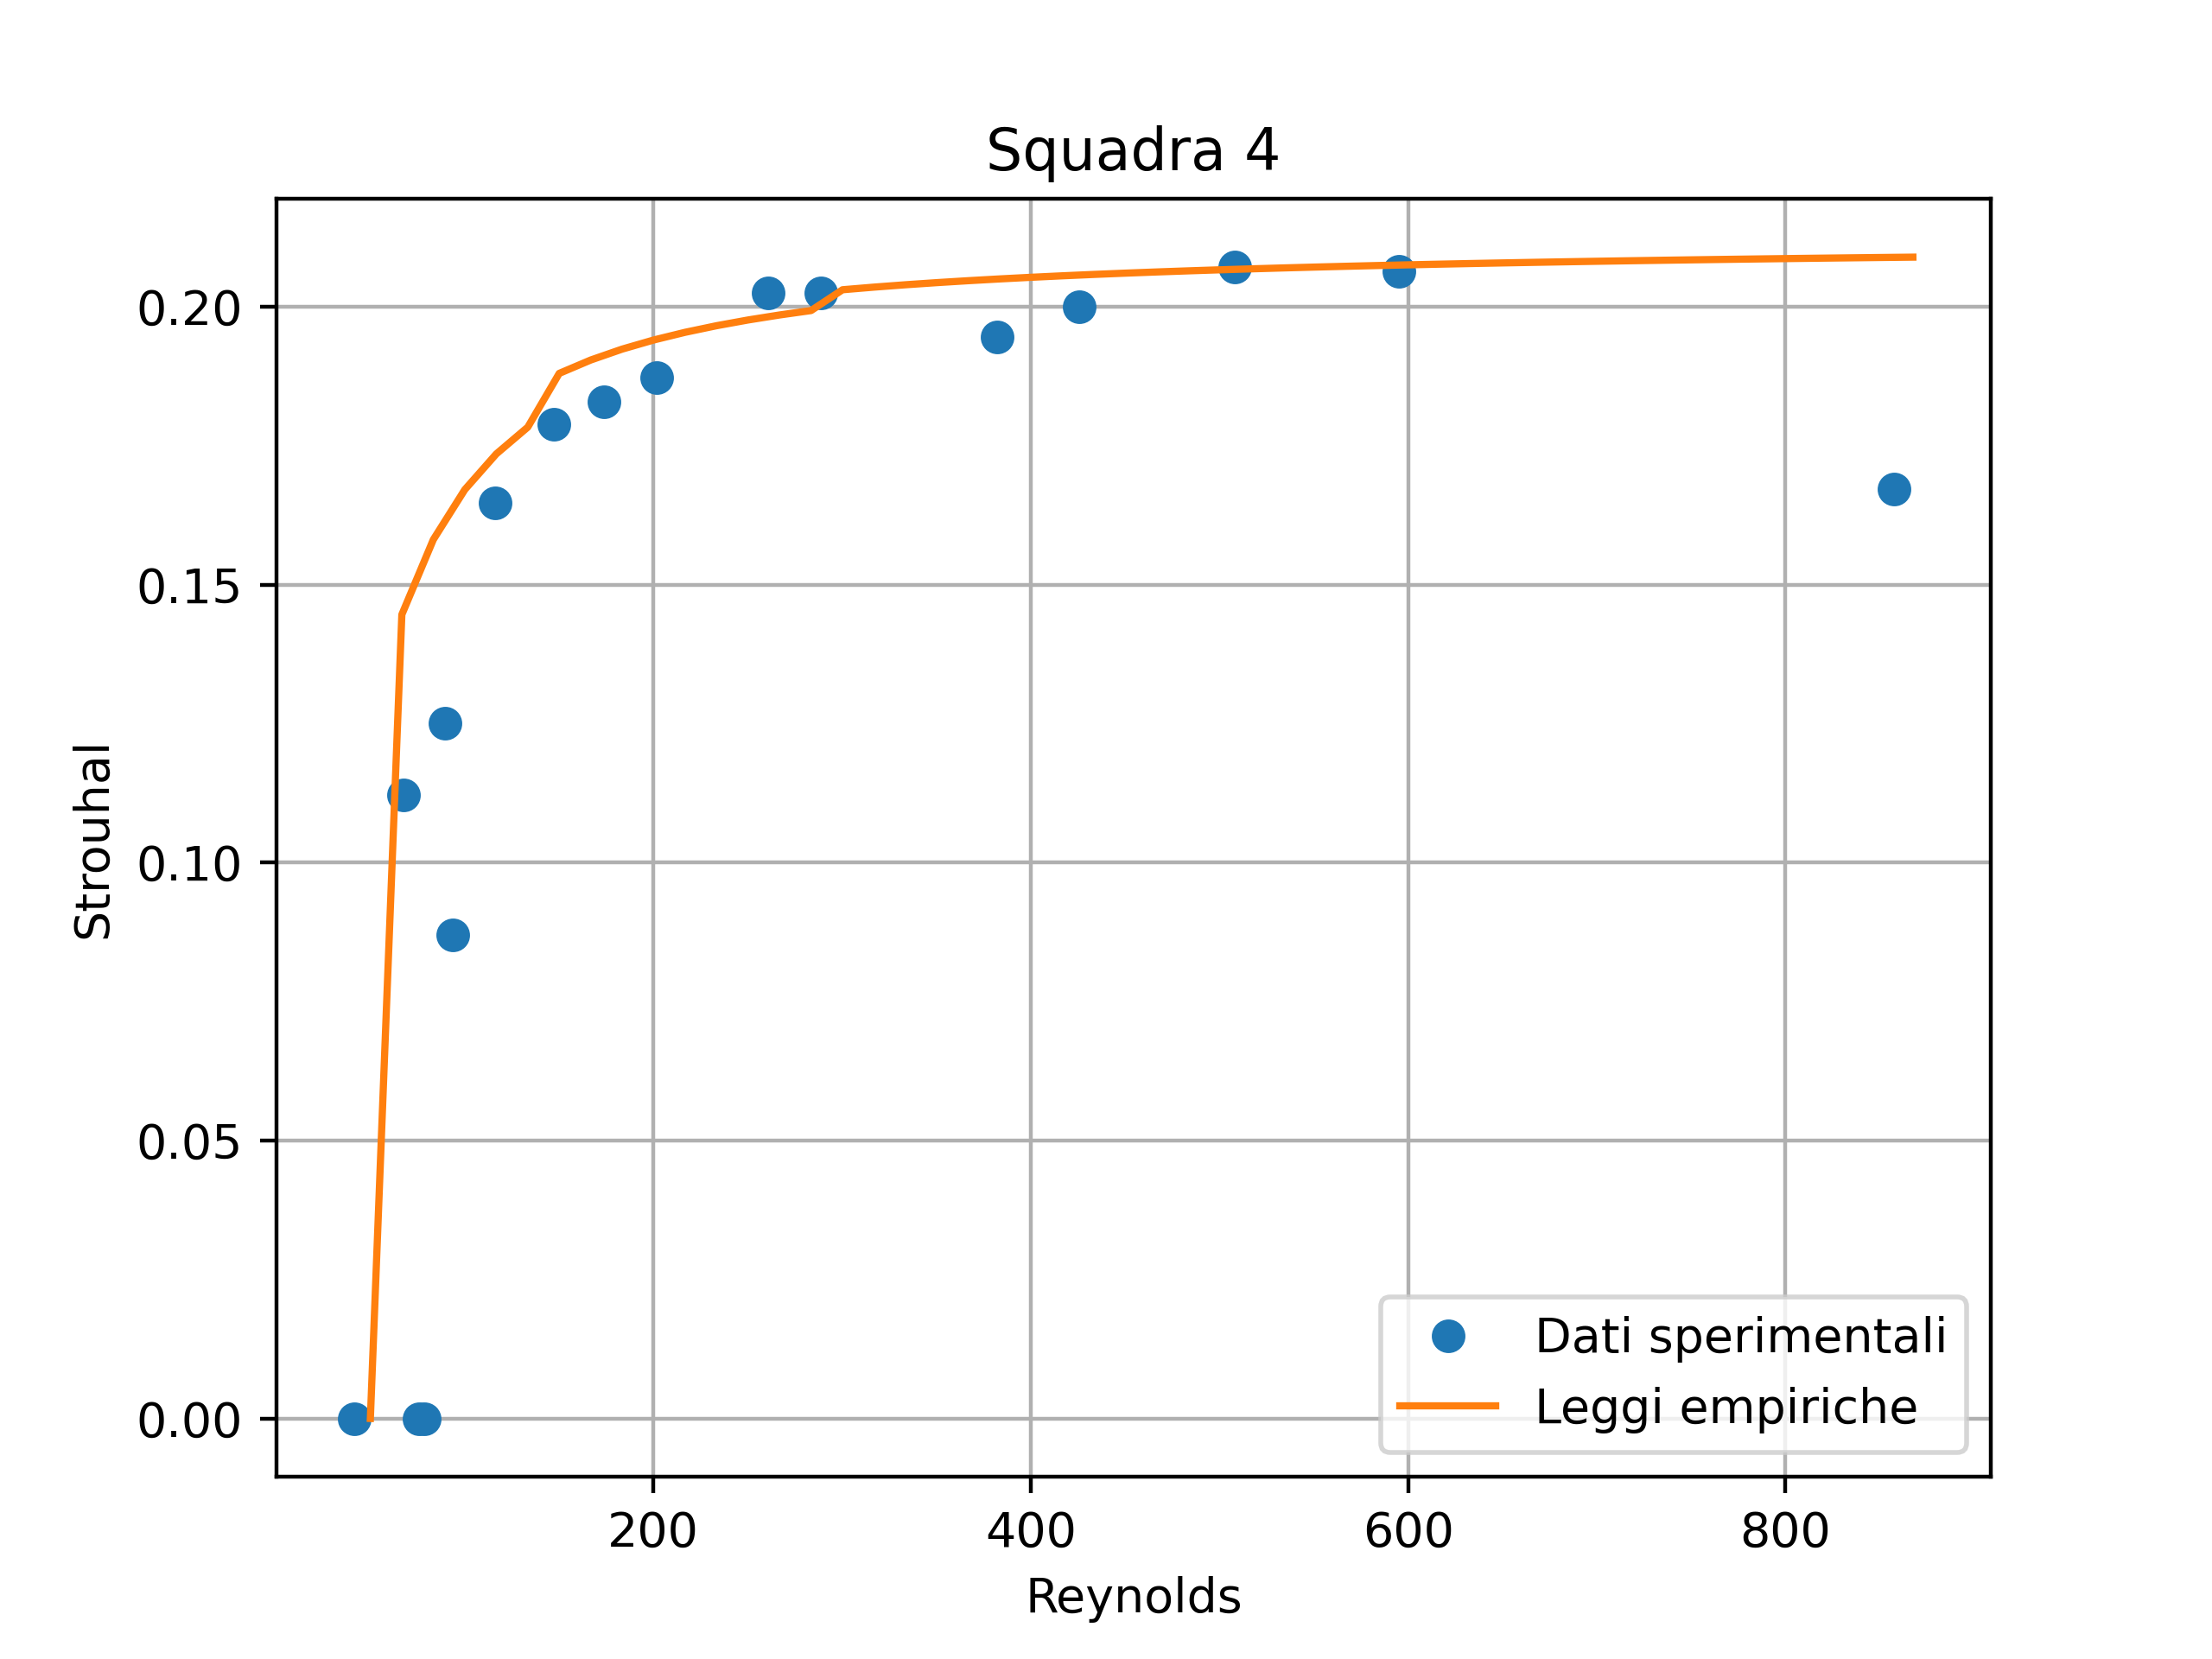
\includegraphics[width=.85\textwidth]{images/10/sq4adim.png}
    \caption{Diagramma $St(Re)$ per la squadra 4}
\end{figure}

\newpage
\noindent Si osserva che per tutte e quattro le squadre i diagrammi Reynolds-Strouhal confermano le leggi empiriche, si può pertanto pensare di raggruppare tutti i dati in un unico diagramma:
\begin{figure}[H]
    \centering
    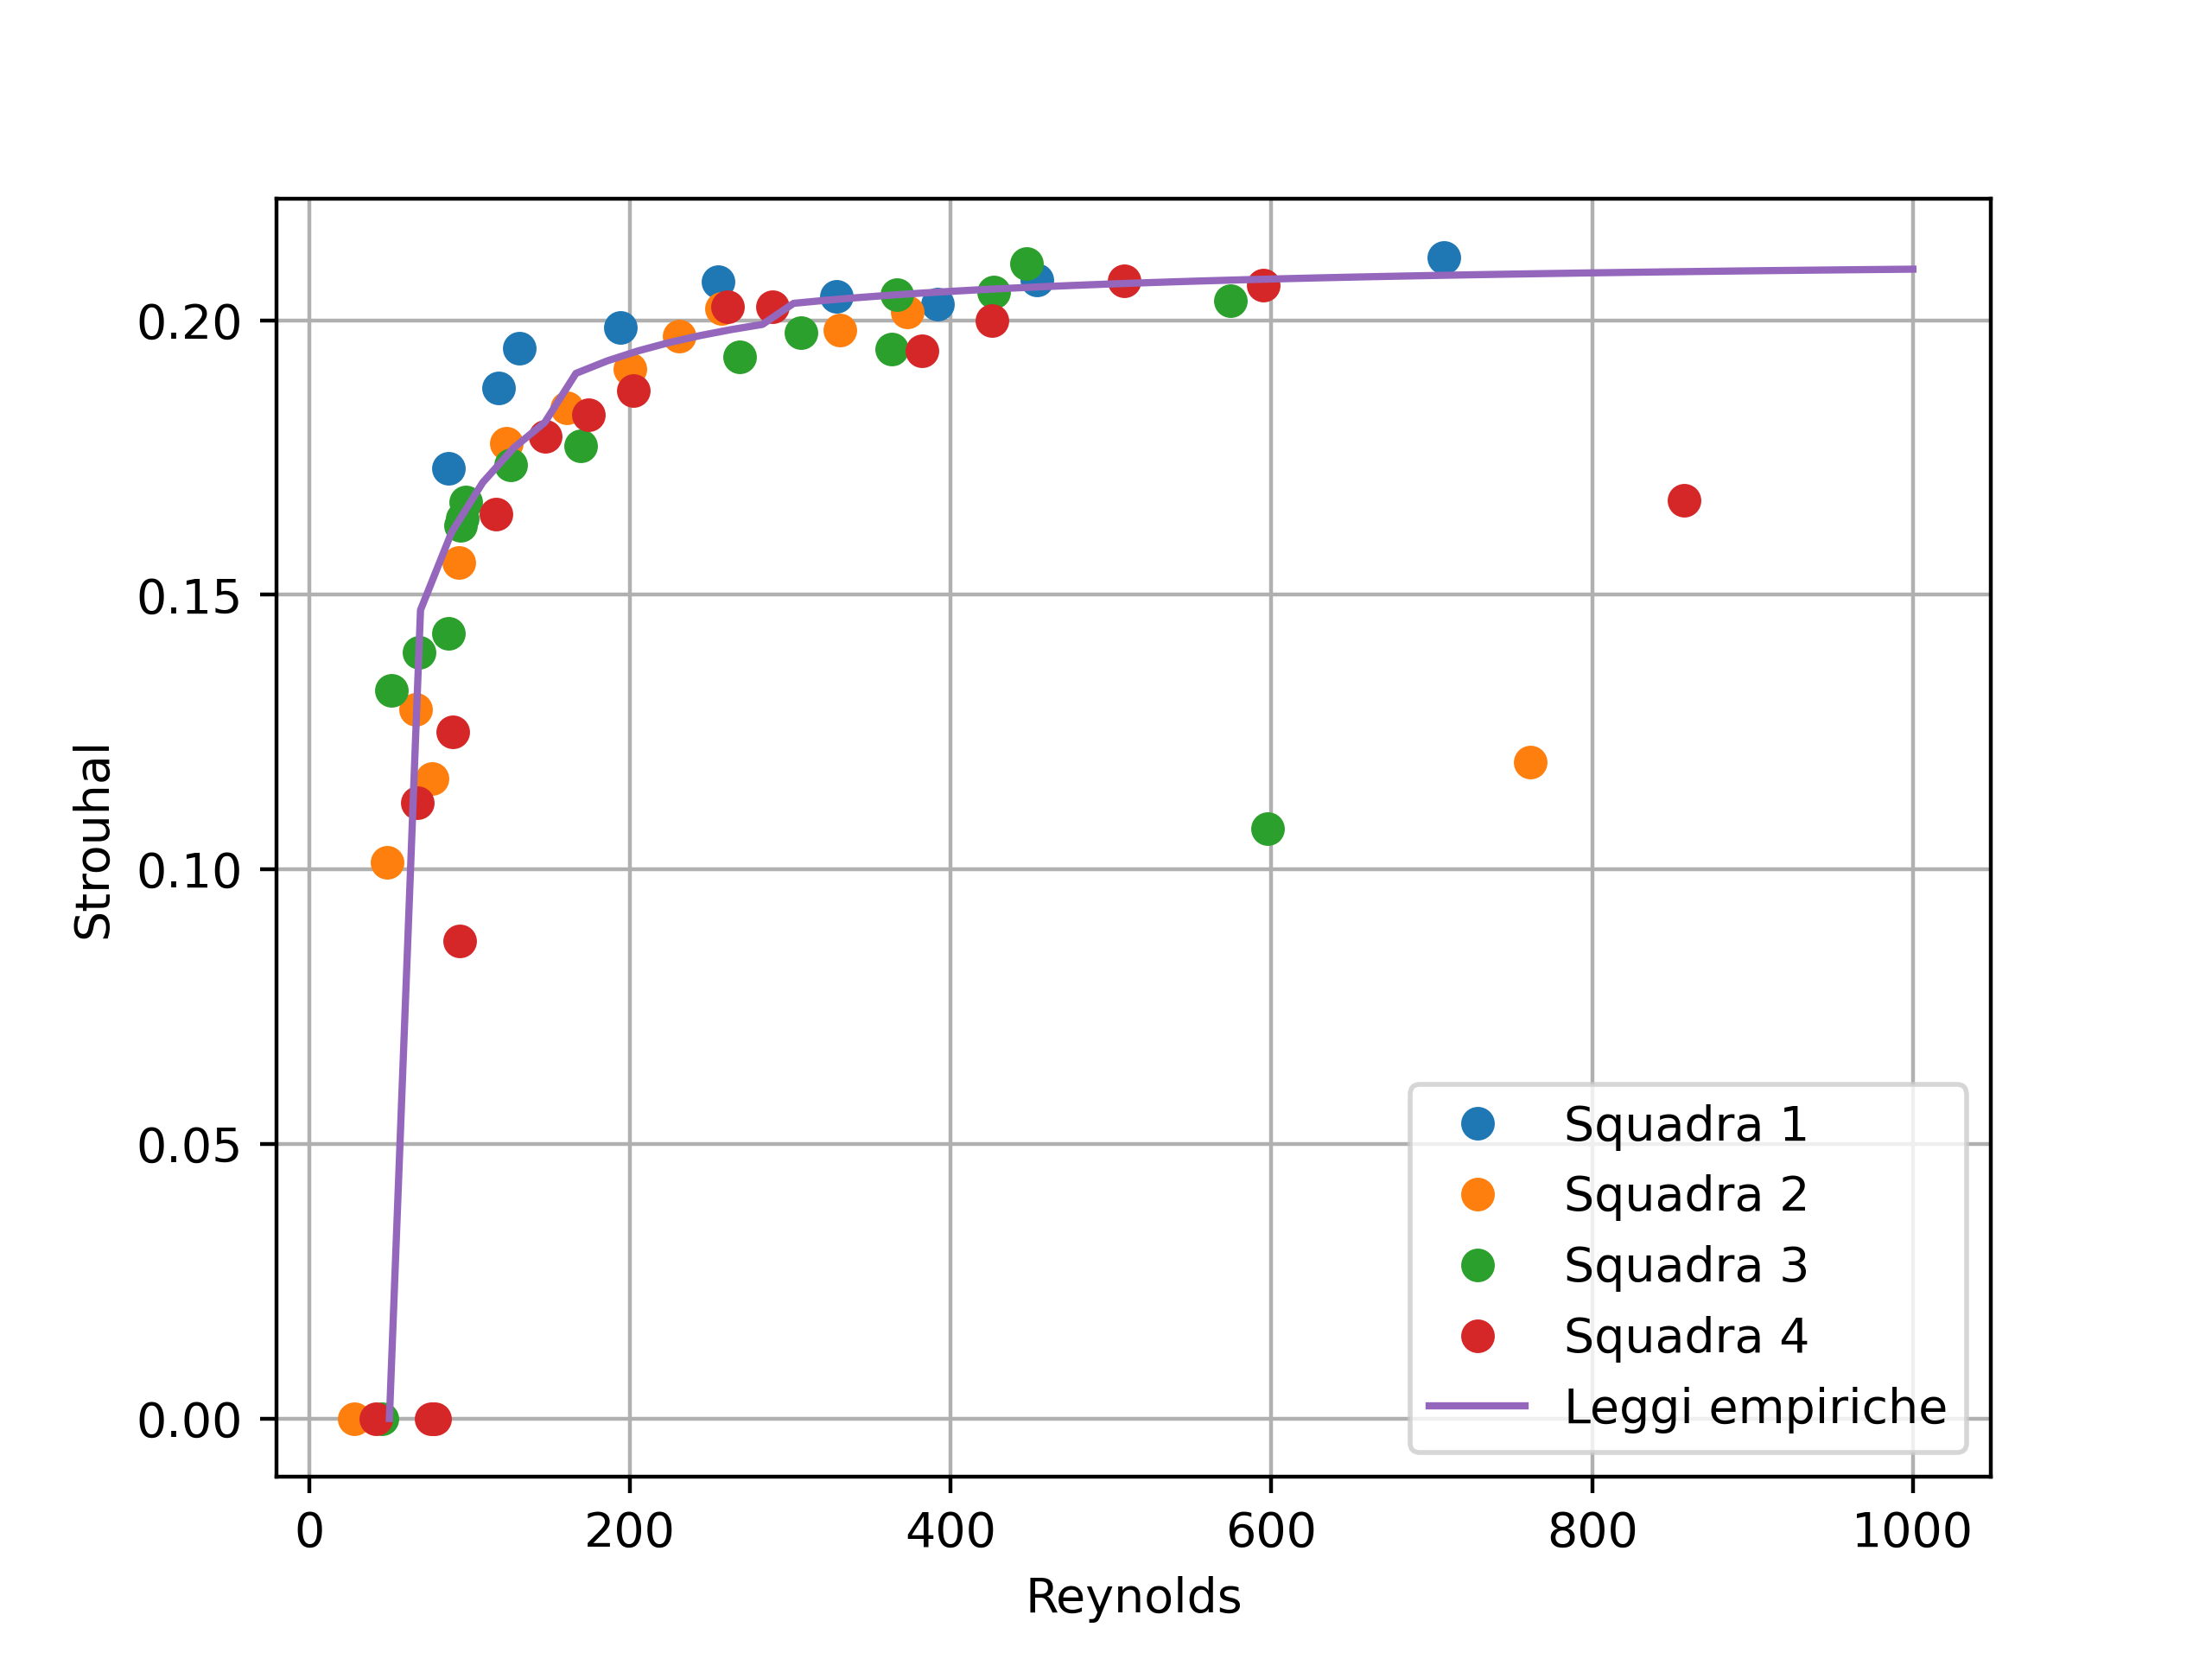
\includegraphics[width=.8\textwidth]{images/10/adim.png}
    \caption{Diagramma $St(Re)$ per le quattro squadre}
\end{figure}

\subsection{Calcolo della frequenza di sfilamento}
Nel presente paragrafo si cerca di determinare la frequenza di shedding $f_s$ dato un profilo di velocità in funzione del tempo $U(t)$ misurato dalla sonda a filo caldo con una frequenza di campionamento di $f_{samp}=10000$ Hz ed un periodo di $T=2$ secondi.
\begin{figure}[H]
    \centering
    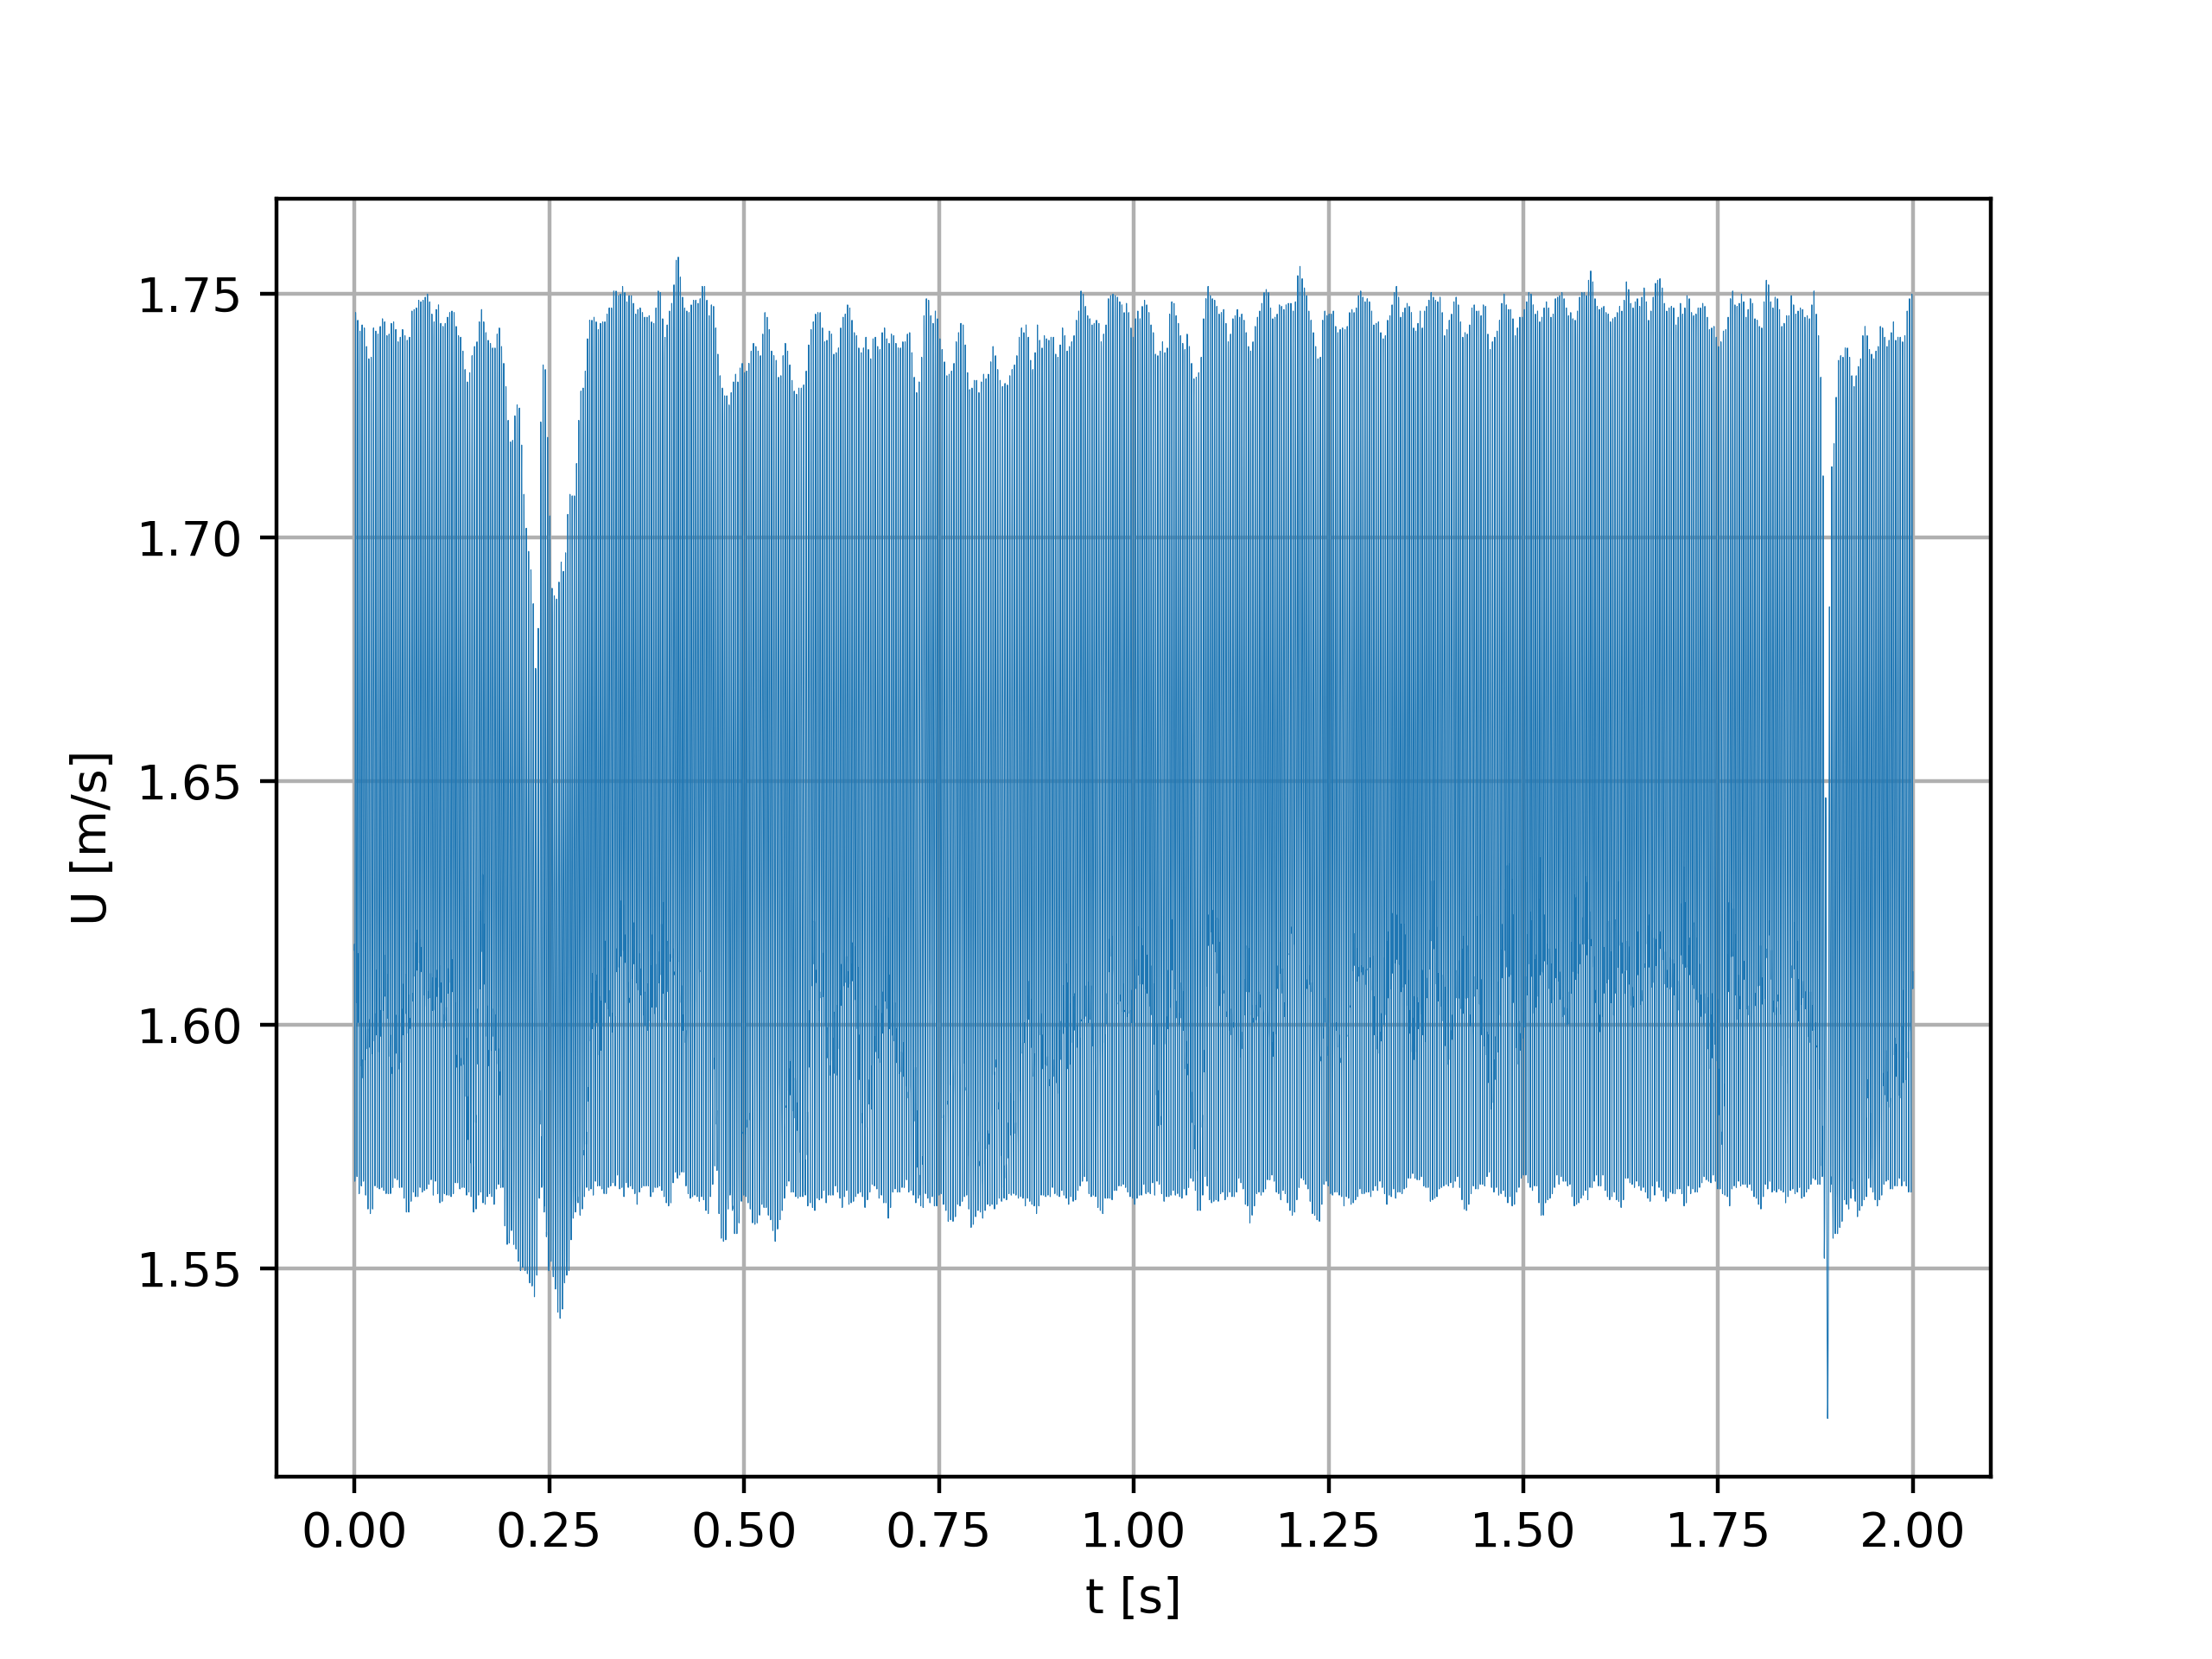
\includegraphics[width=.55\textwidth]{images/10/timeseries.png}
\end{figure}

\noindent È subito possibile ricavare la velocità media e la deviazione standard:
\begin{equation*}
    \overline U = 1.65\ \text{m/s} \qquad u_{rms} = 0.061\ \text{m/s}
\end{equation*}
Nonostante il profilo di velocità sembri avere un andamento casuale, in realtà permette di estrarre, tramite il metodo di Welch, il contenuto energetico associato ad ogni frequenza, e quindi determinare la frequenza di sfilamento $f_s$.\\\\
Applicando il metodo di Welch, si ottiene il seguente diagramma:
\begin{figure}[H]
    \centering
    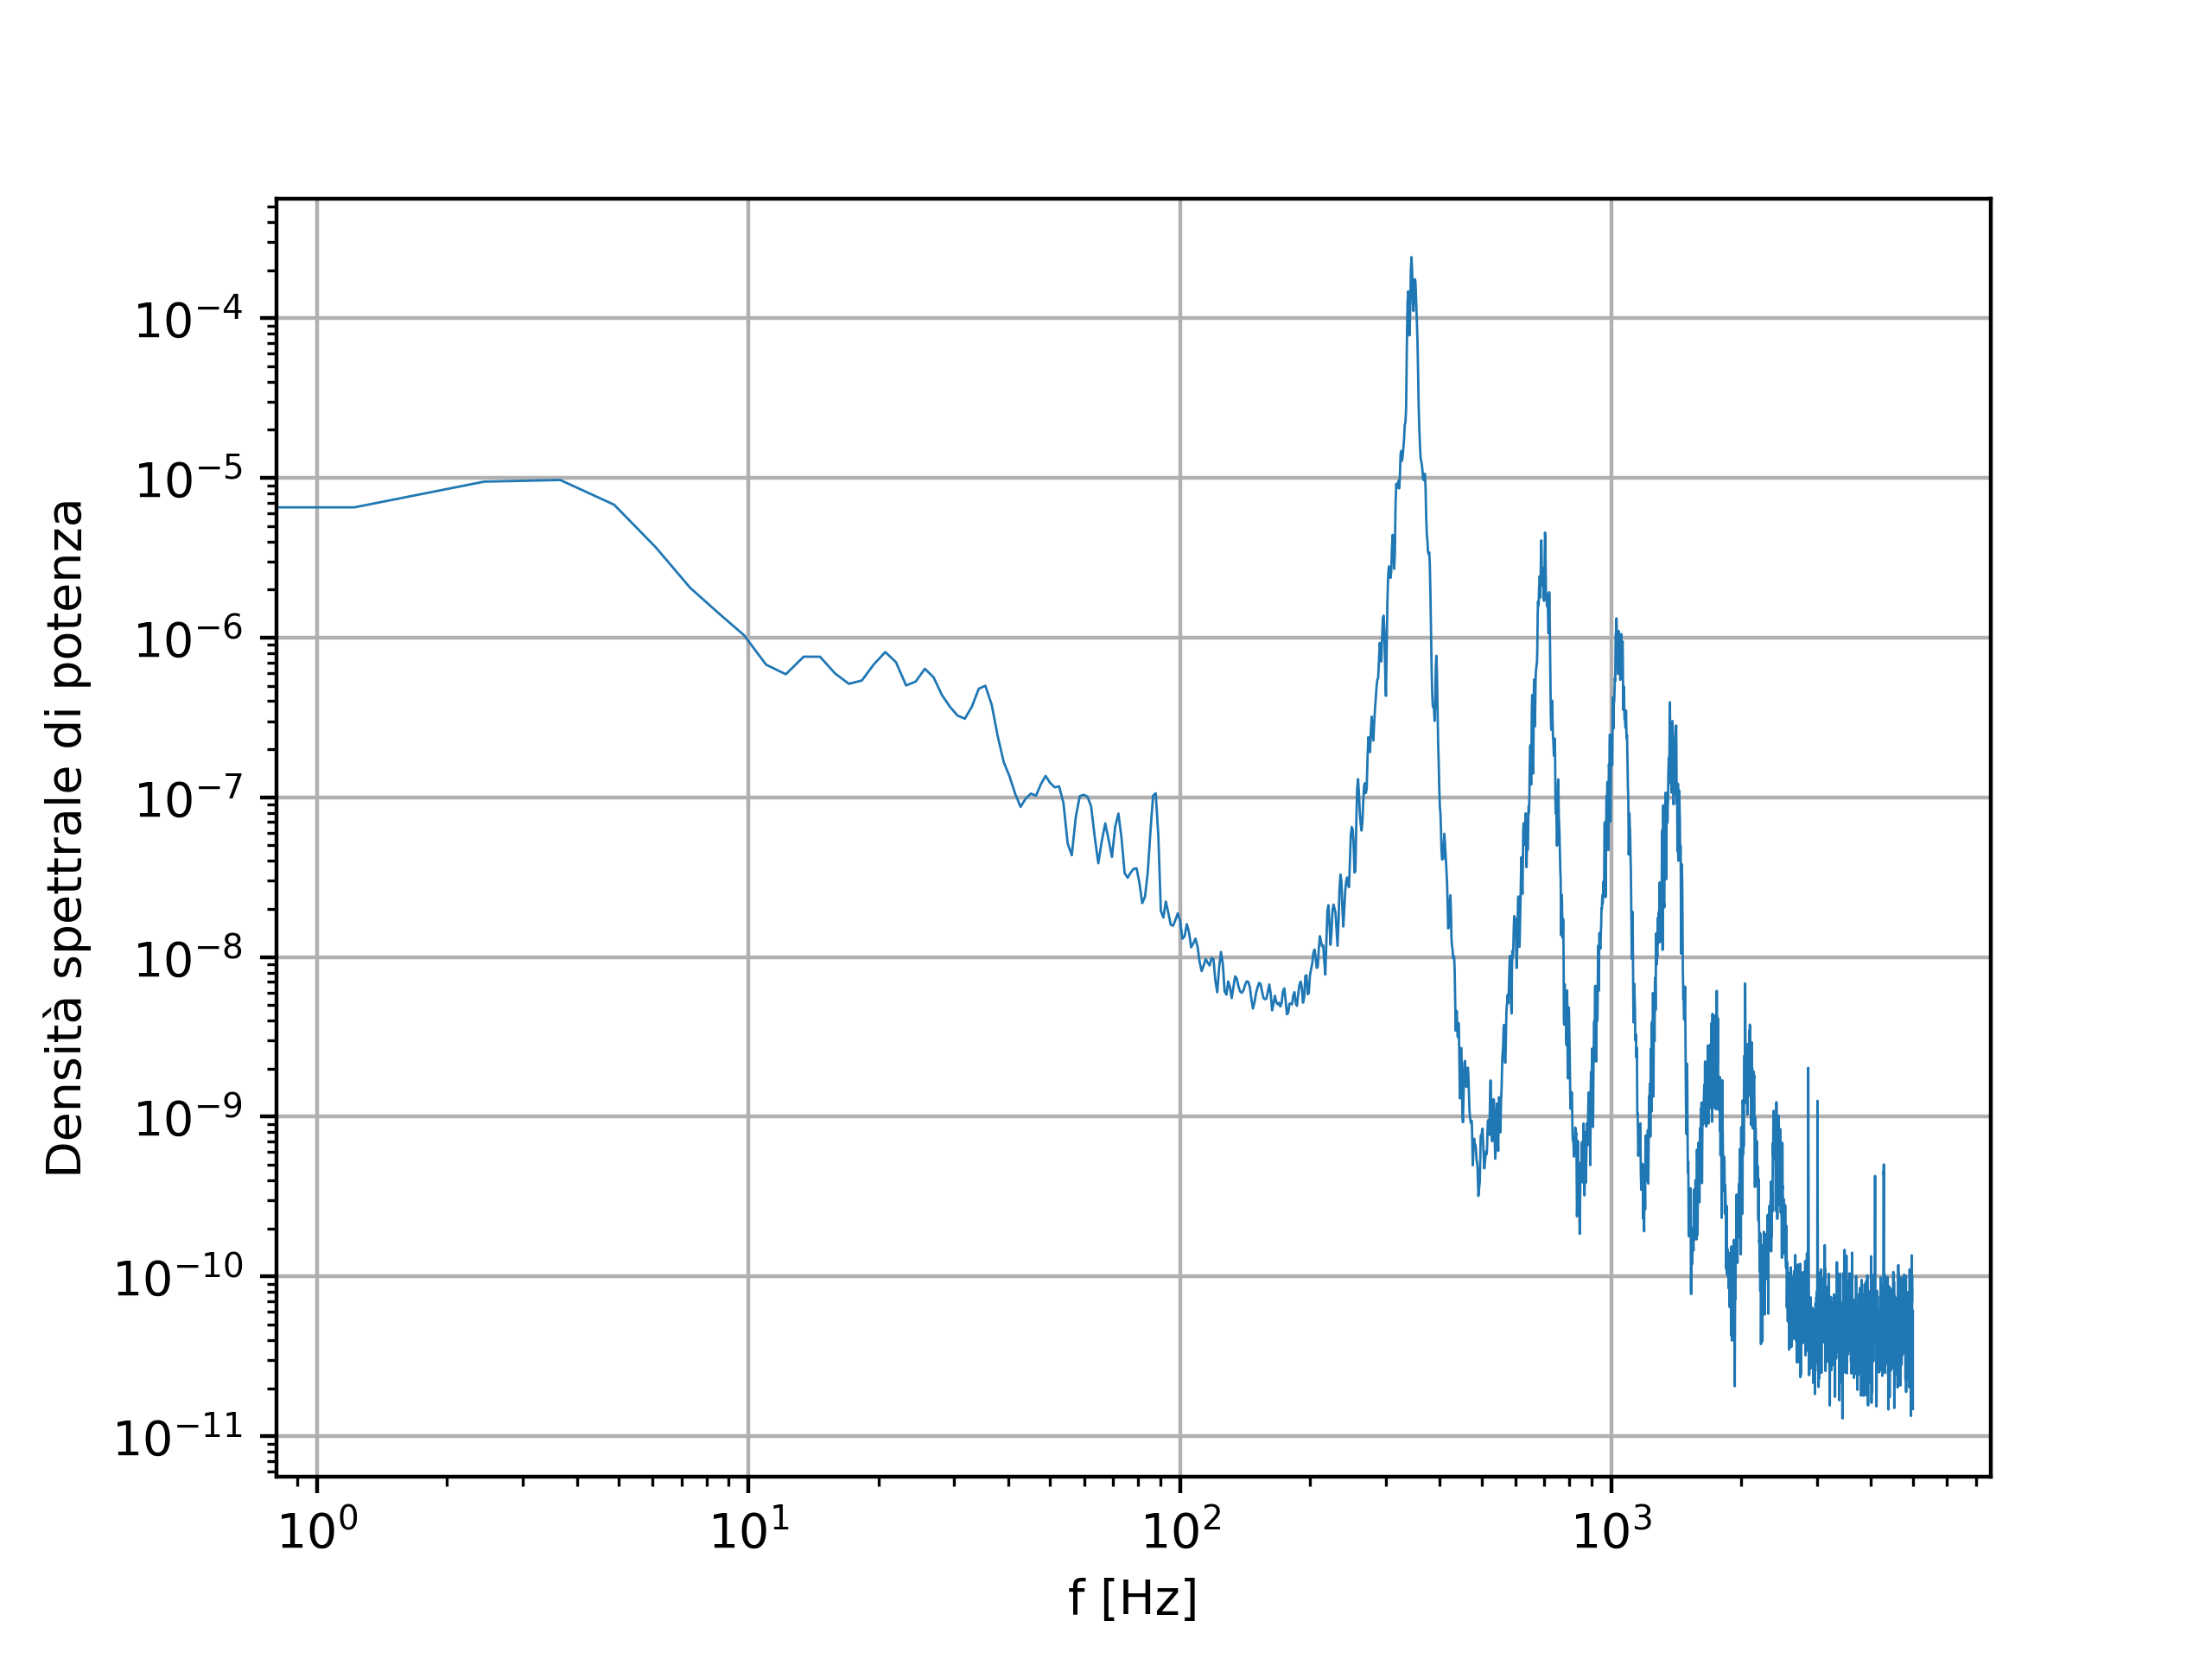
\includegraphics[width=.9\textwidth]{images/10/welch.png}
    \caption{Spettro di potenza}
\end{figure}

\noindent Dal quale, identificando il primo picco di energia, è possibile ricavare il valore della frequenza di sfilamento (nel caso in esame, il picco corrisponde al massimo dell'energia per ogni frequenza). Si ottiene quindi una frequenza di sfilamento:
\begin{equation*}
    f_s = 344.24\ \text{Hz}
\end{equation*}
I picchi successivi presenti nel diagramma sono posizionati a frequenze multiple della frequenza di sfilamento.

\newpage
\subsection{Analisi di convergenza}
Considerando il profilo di velocità precedentemente analizzato, è utile indagare il numero di punti necessario per la convergenza statistica della velocità media e dei vari momenti statistici.\\\\
Per fare ciò, si traccia un diagramma che ha come ascisse il numero di punti $n$ da considerare e come ordinate il valore della velocità media $\overline U$ che si ottiene considerando i primi $n$ punti:
\begin{figure}[H]
    \centering
    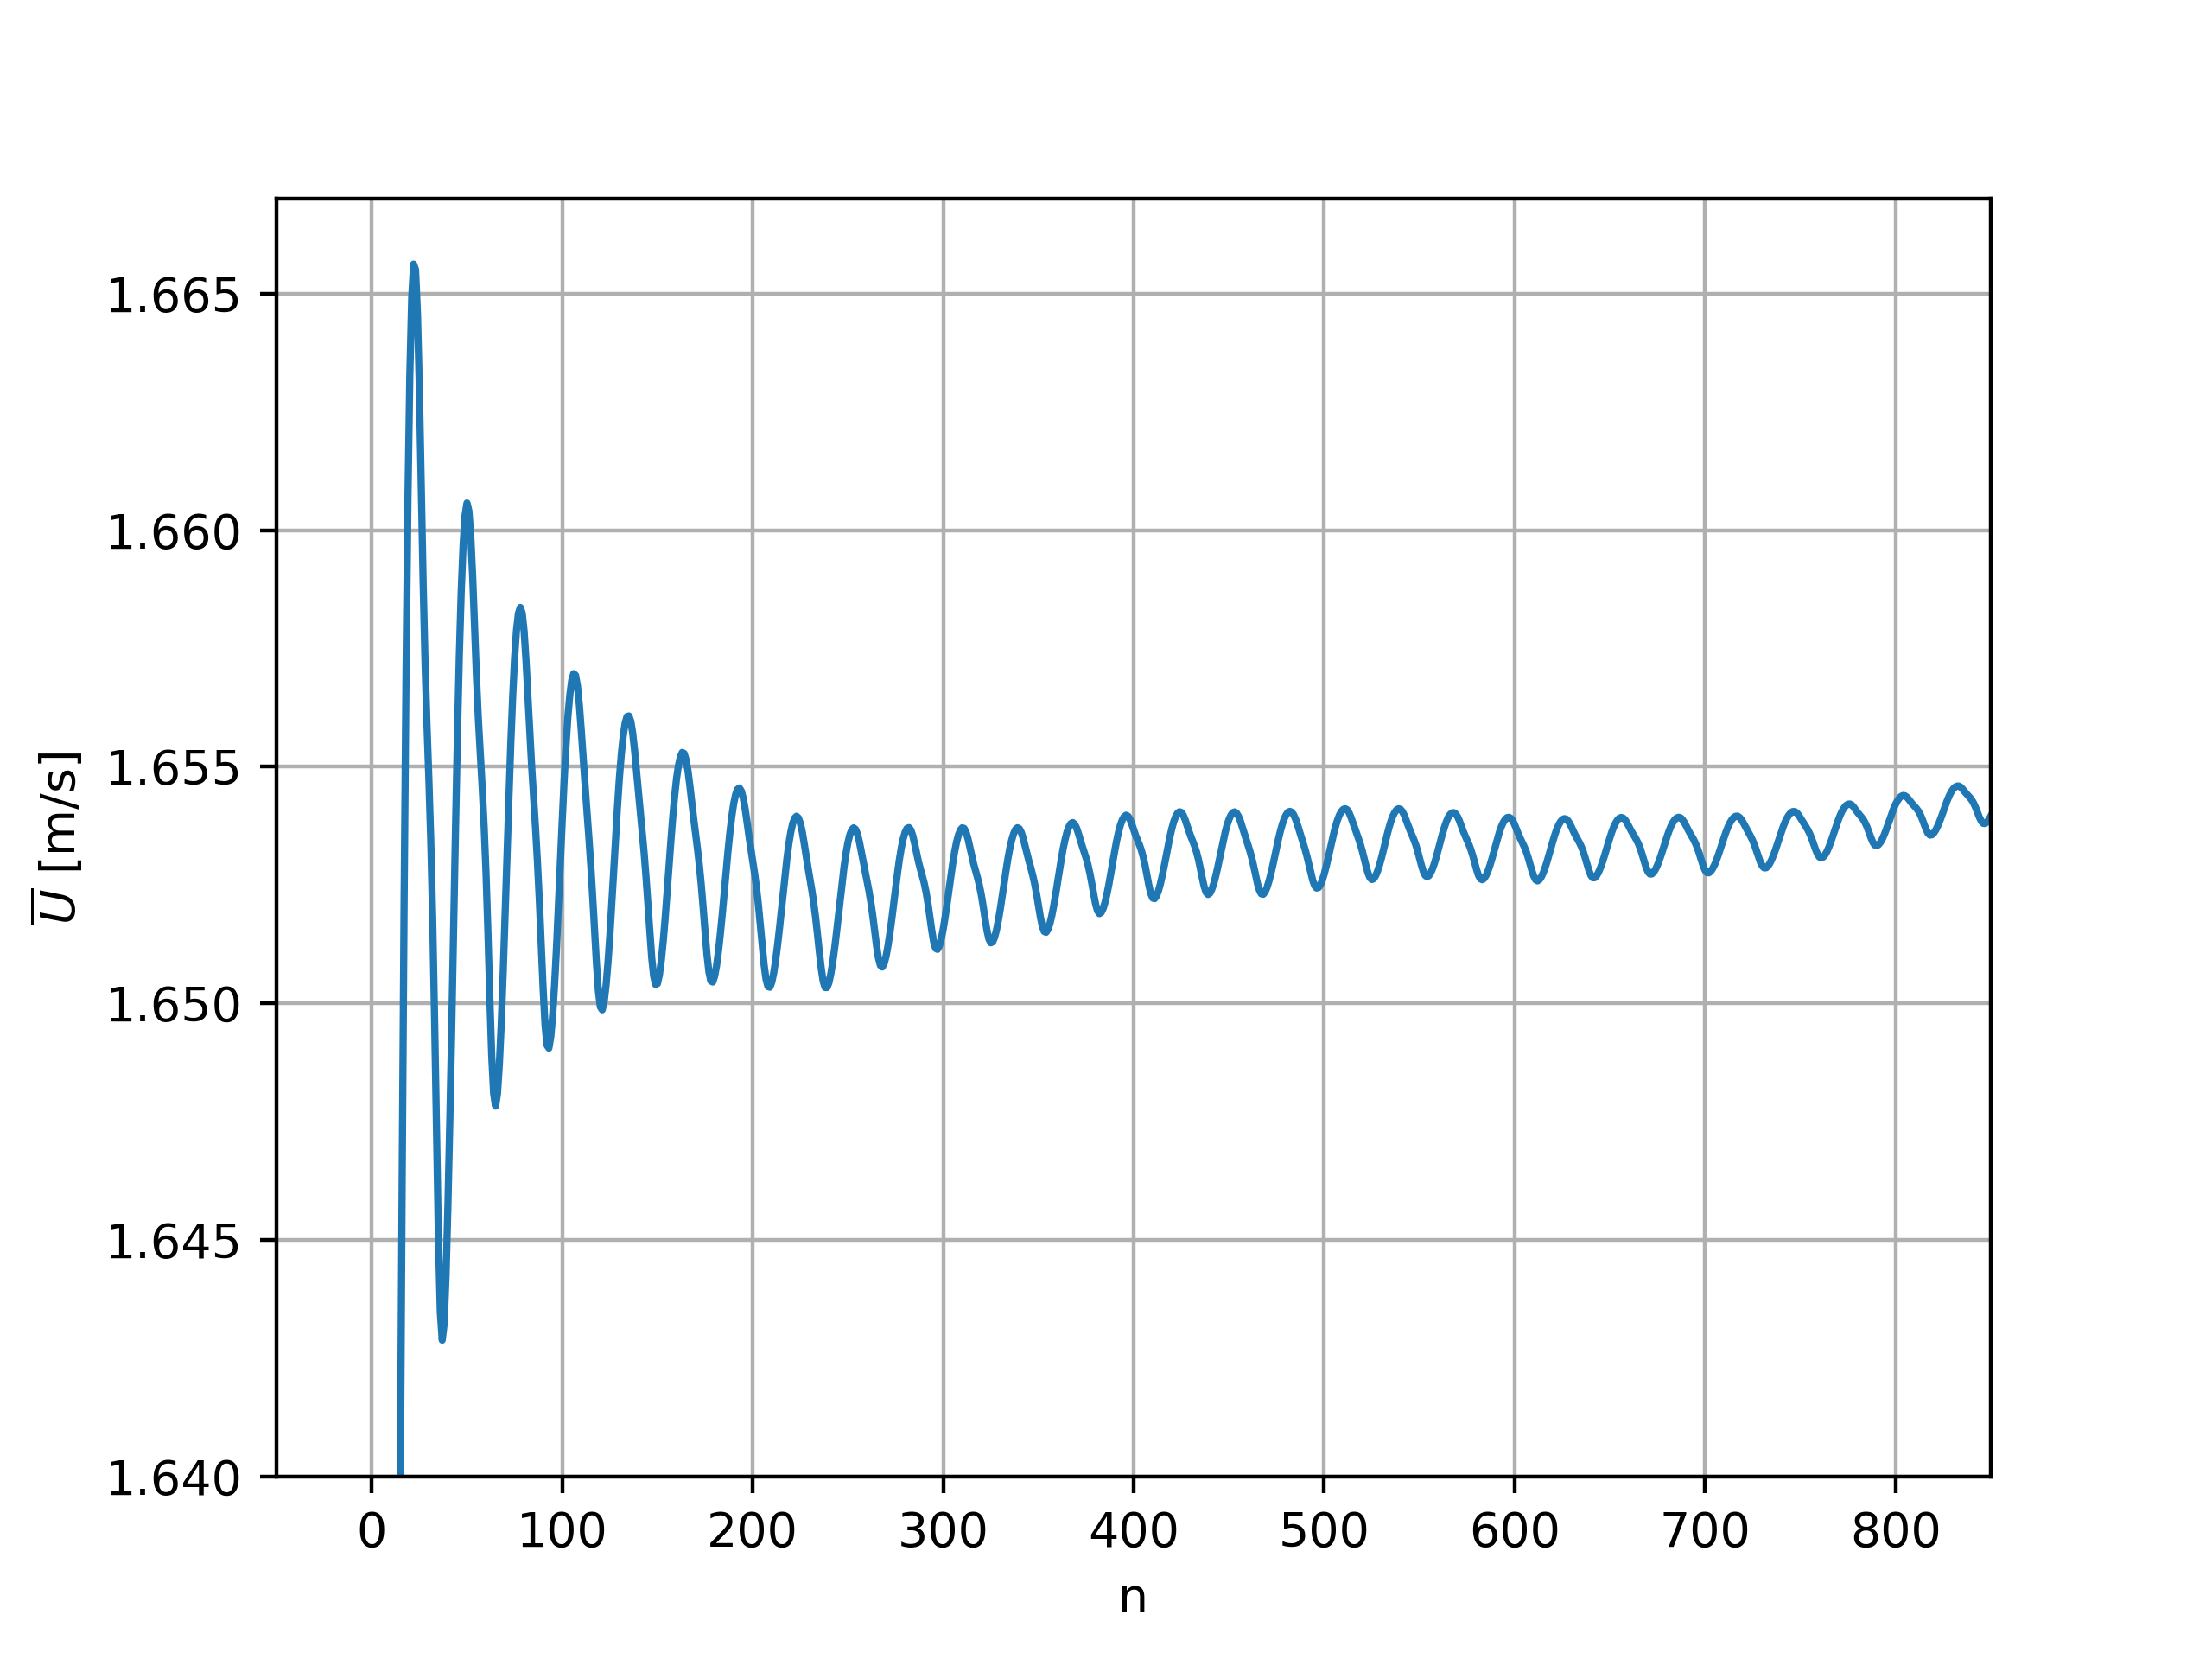
\includegraphics[width=.48\textwidth]{images/10/conv2.png}
    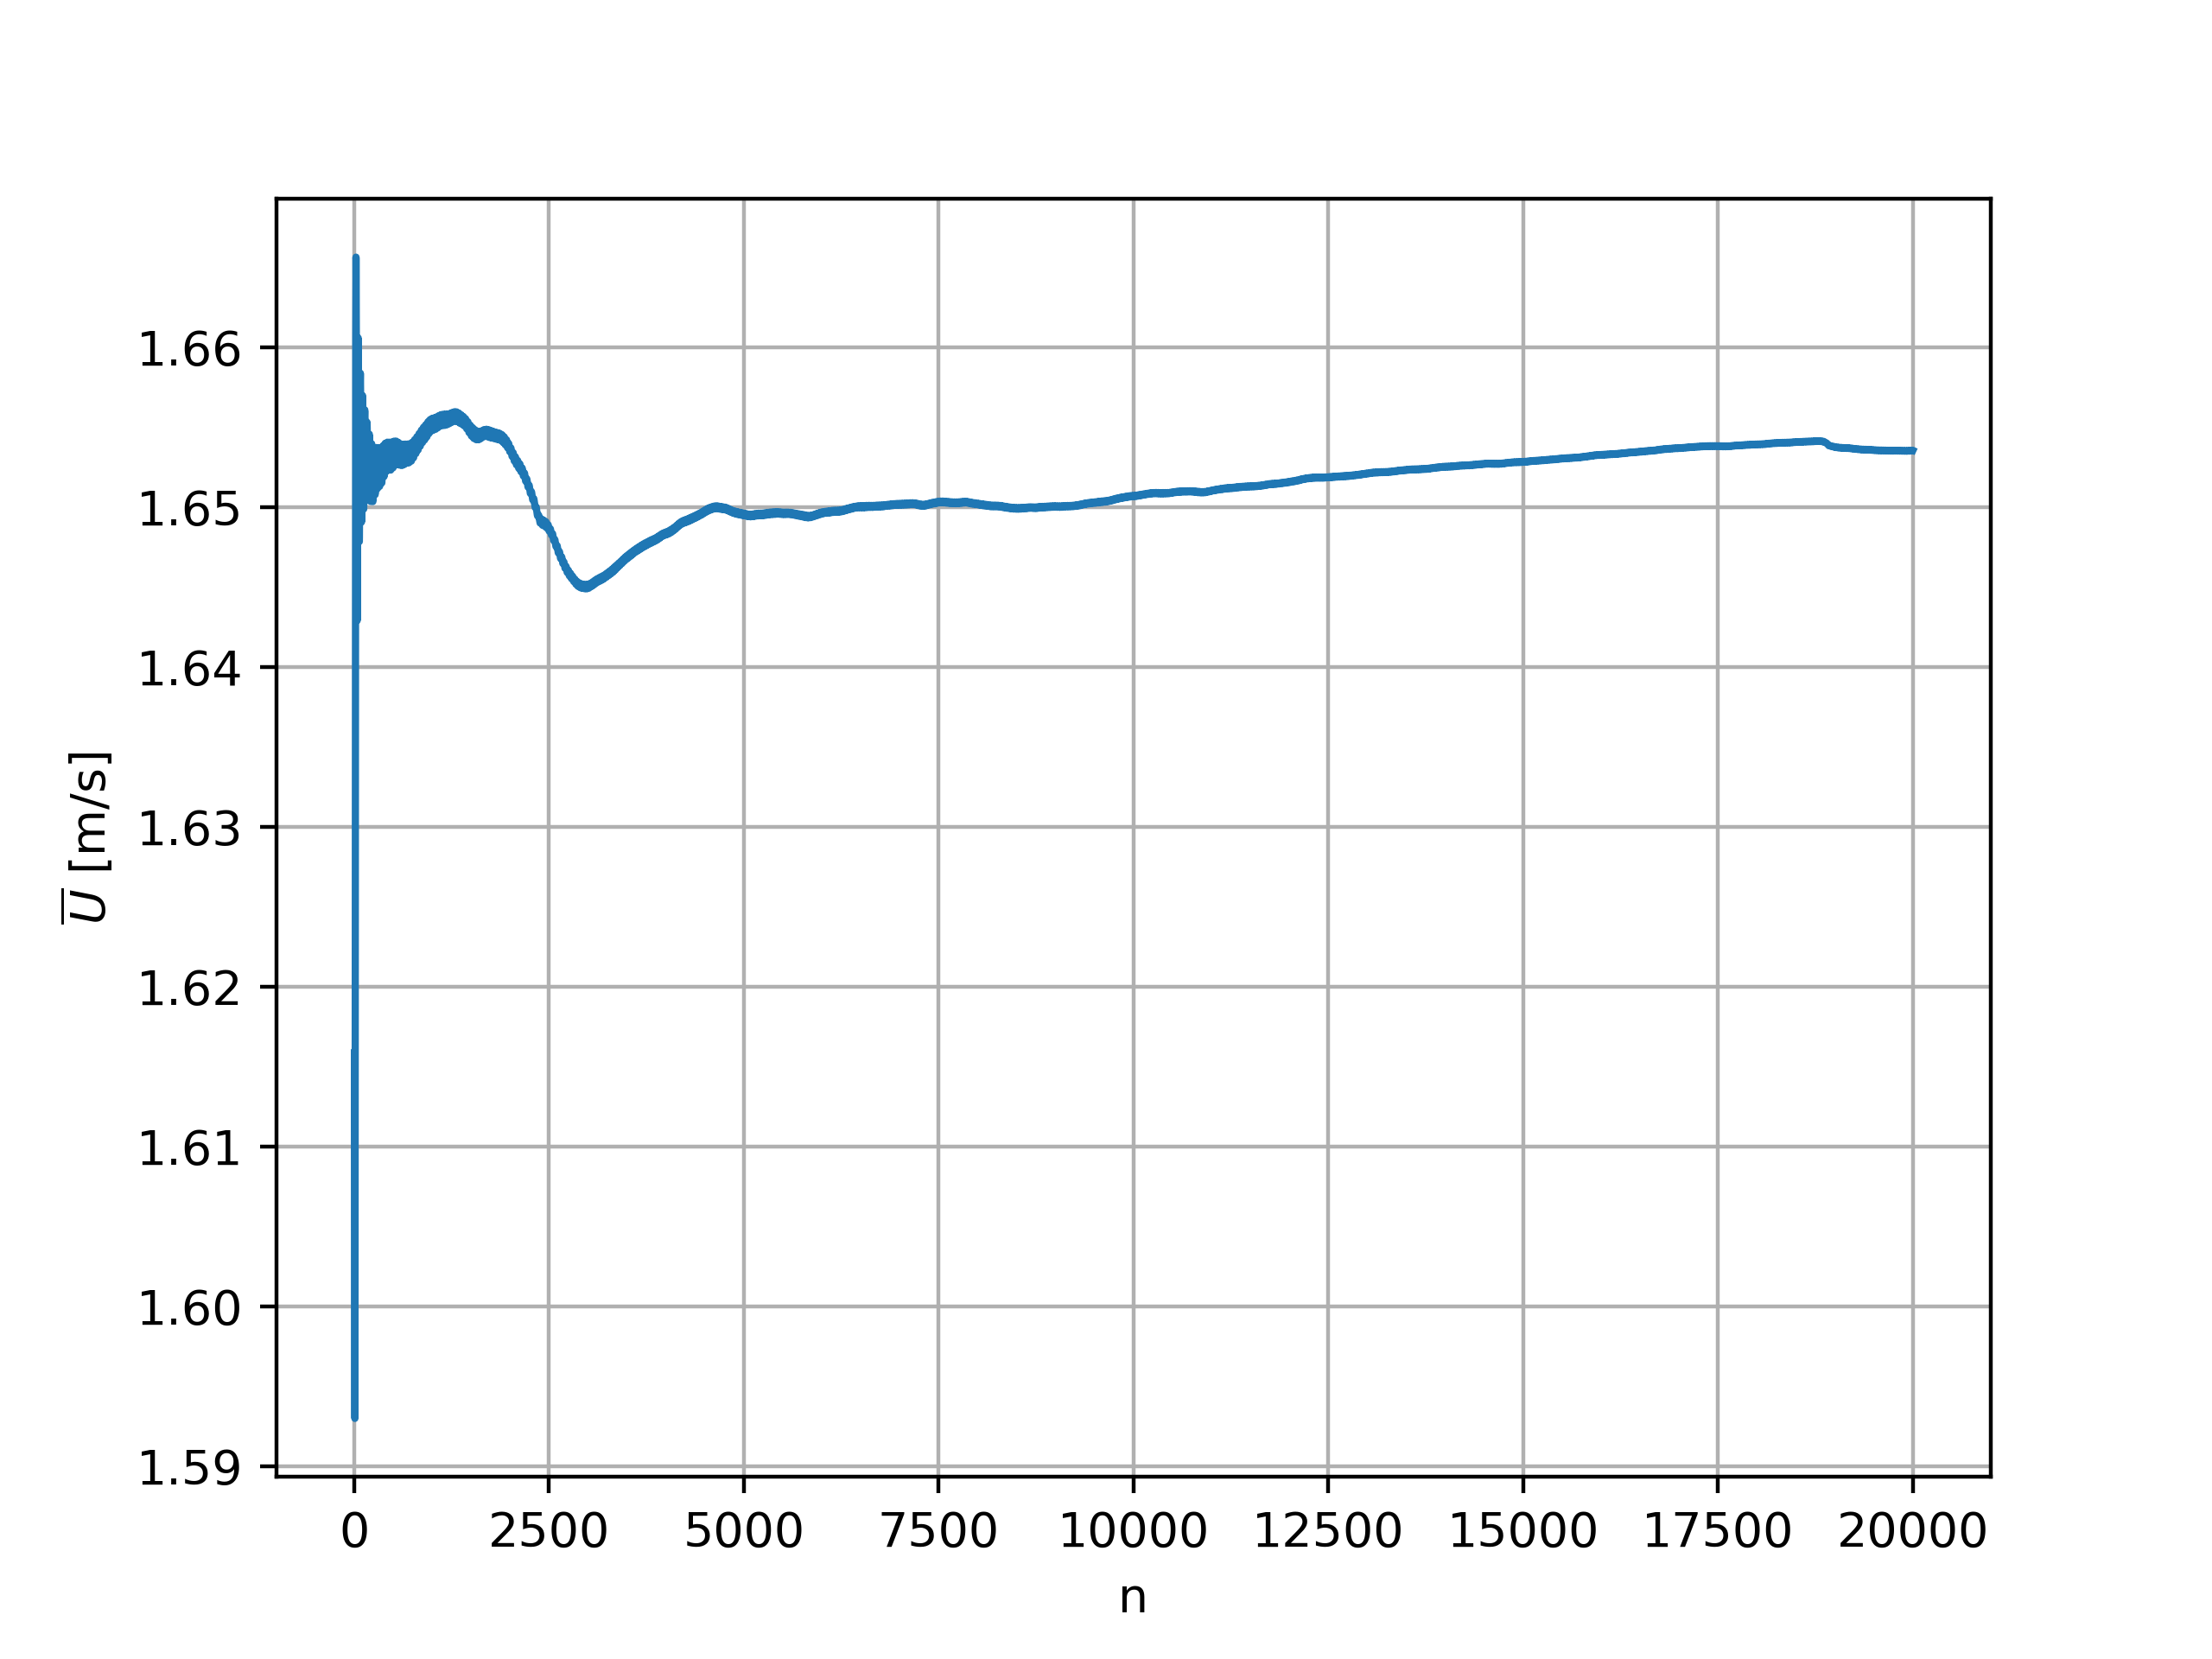
\includegraphics[width=.48\textwidth]{images/10/conv1.png}
    \caption{Analisi di convergenza della velocità media}
\end{figure}

\noindent Si fa lo stesso per la deviazione standard della velocità $u_{rms}$:
\begin{figure}[H]
    \centering
    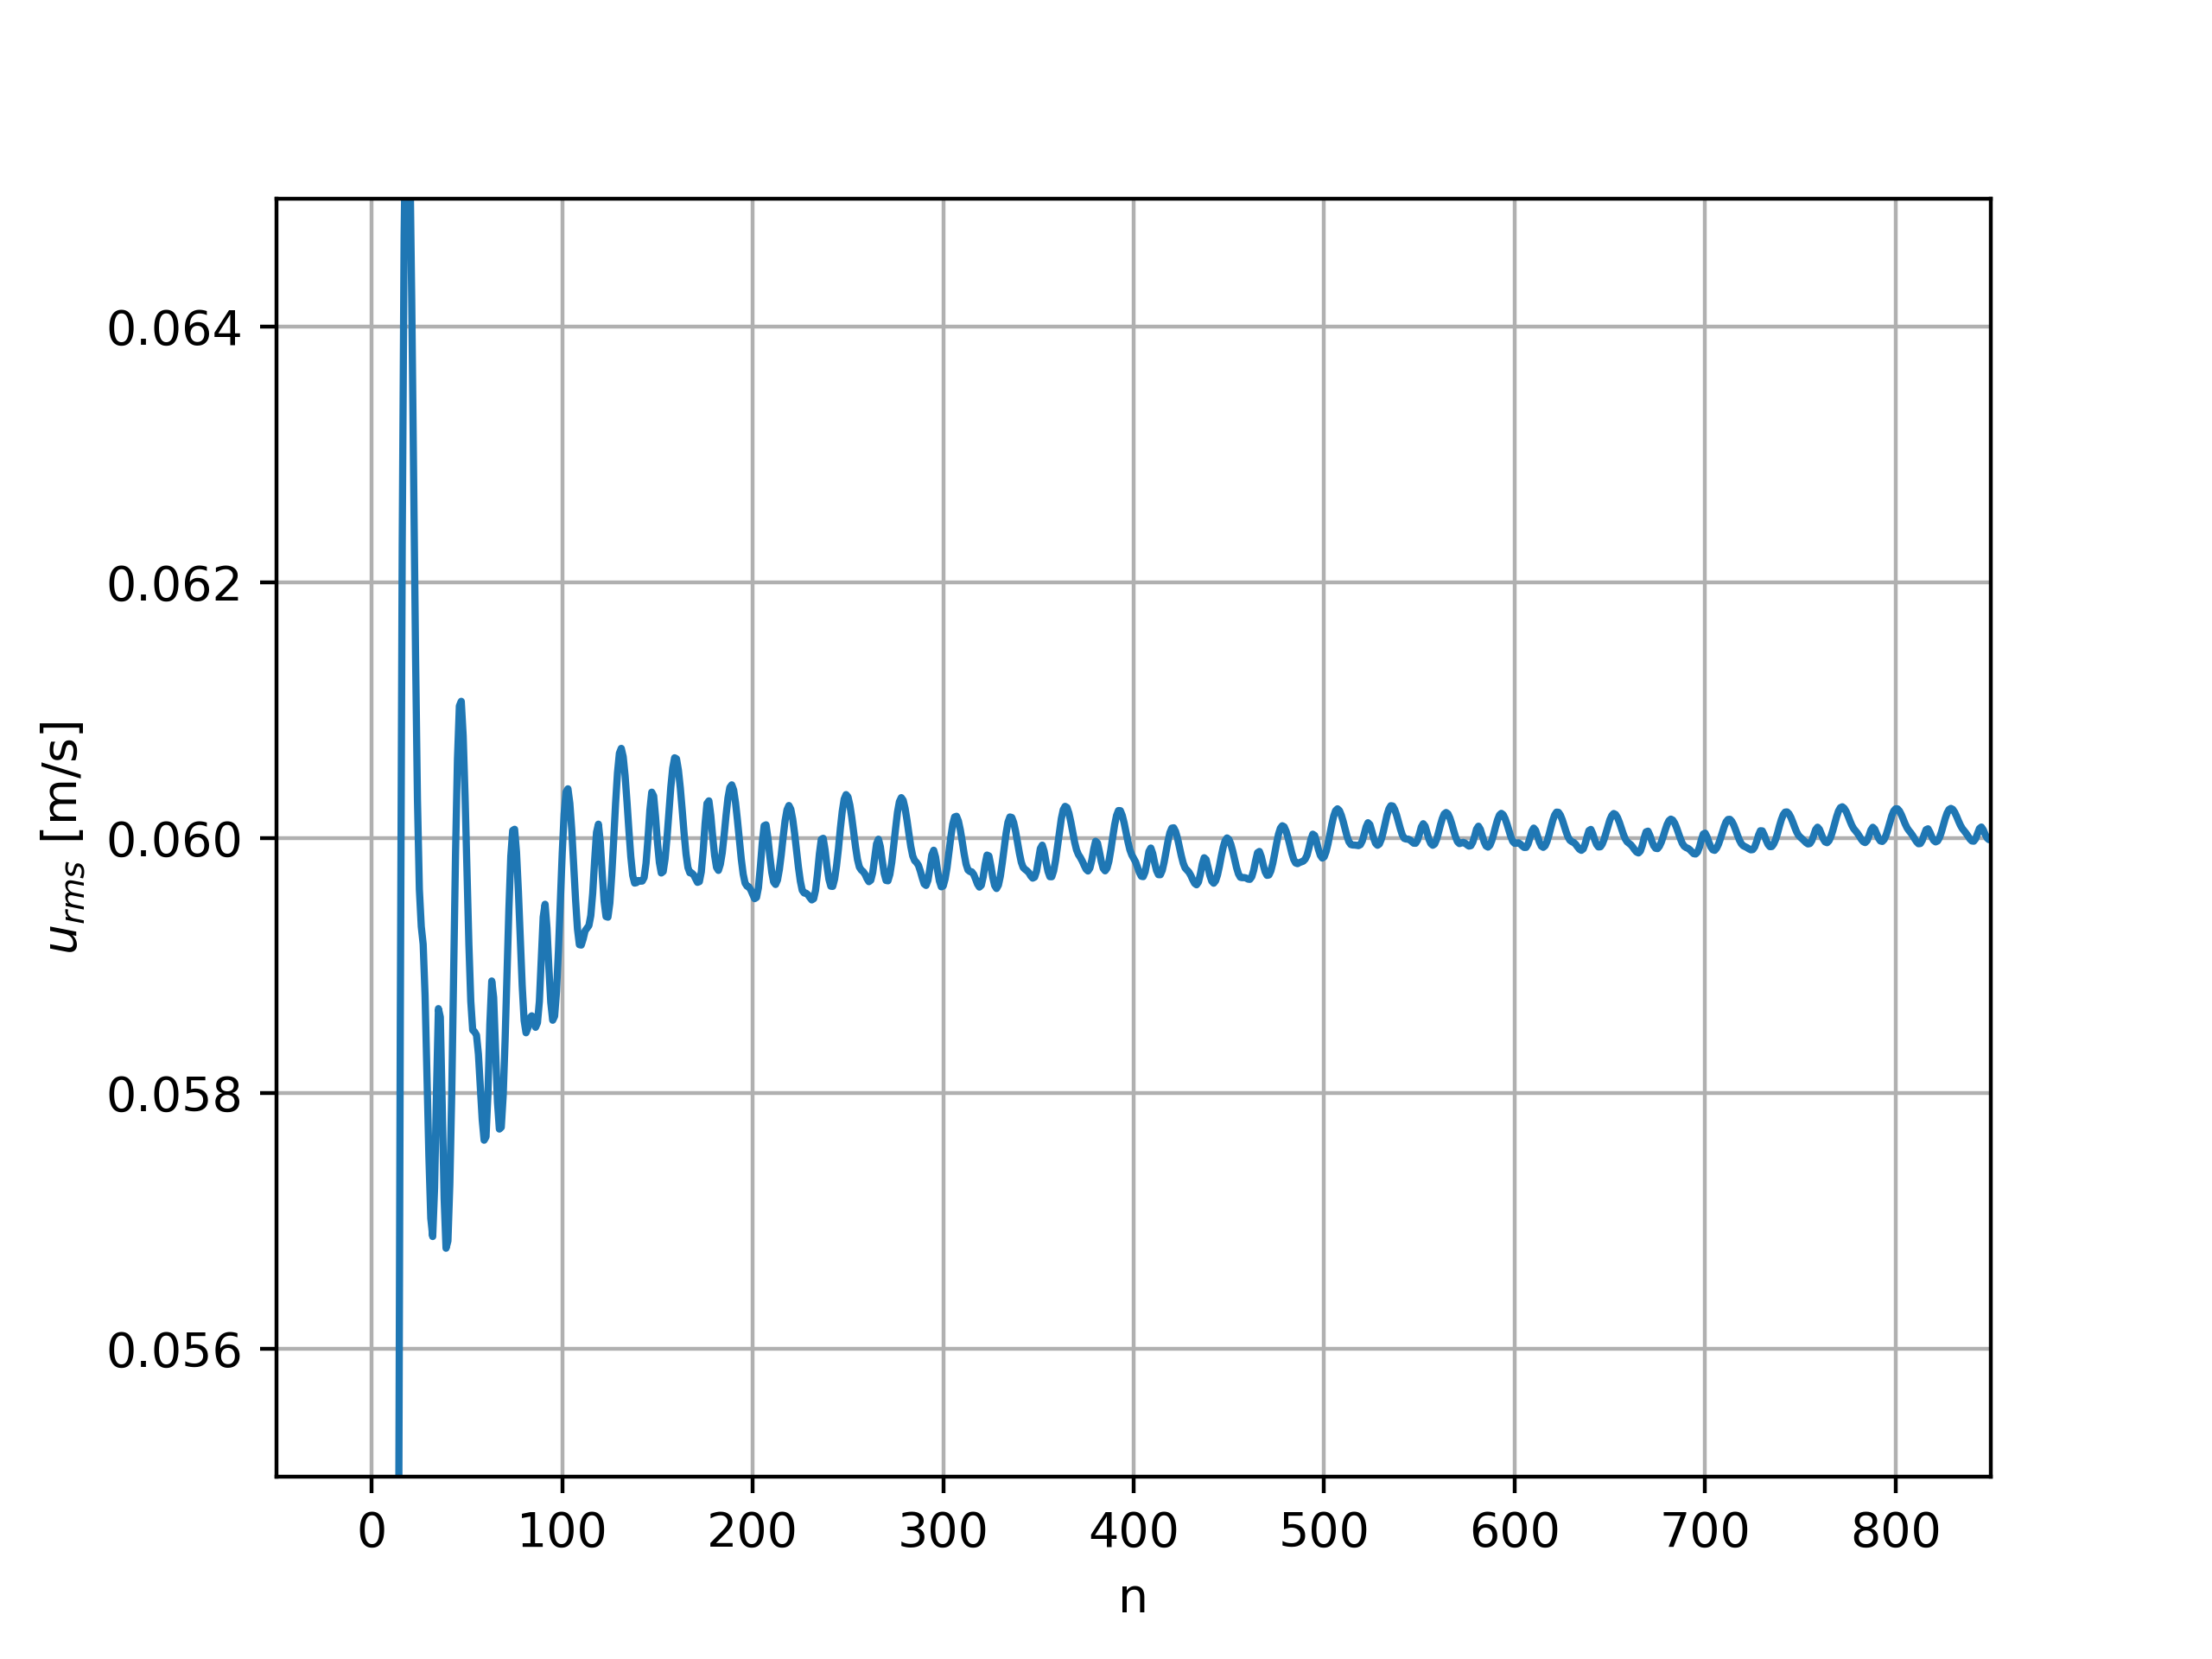
\includegraphics[width=.48\textwidth]{images/10/conv4.png}
    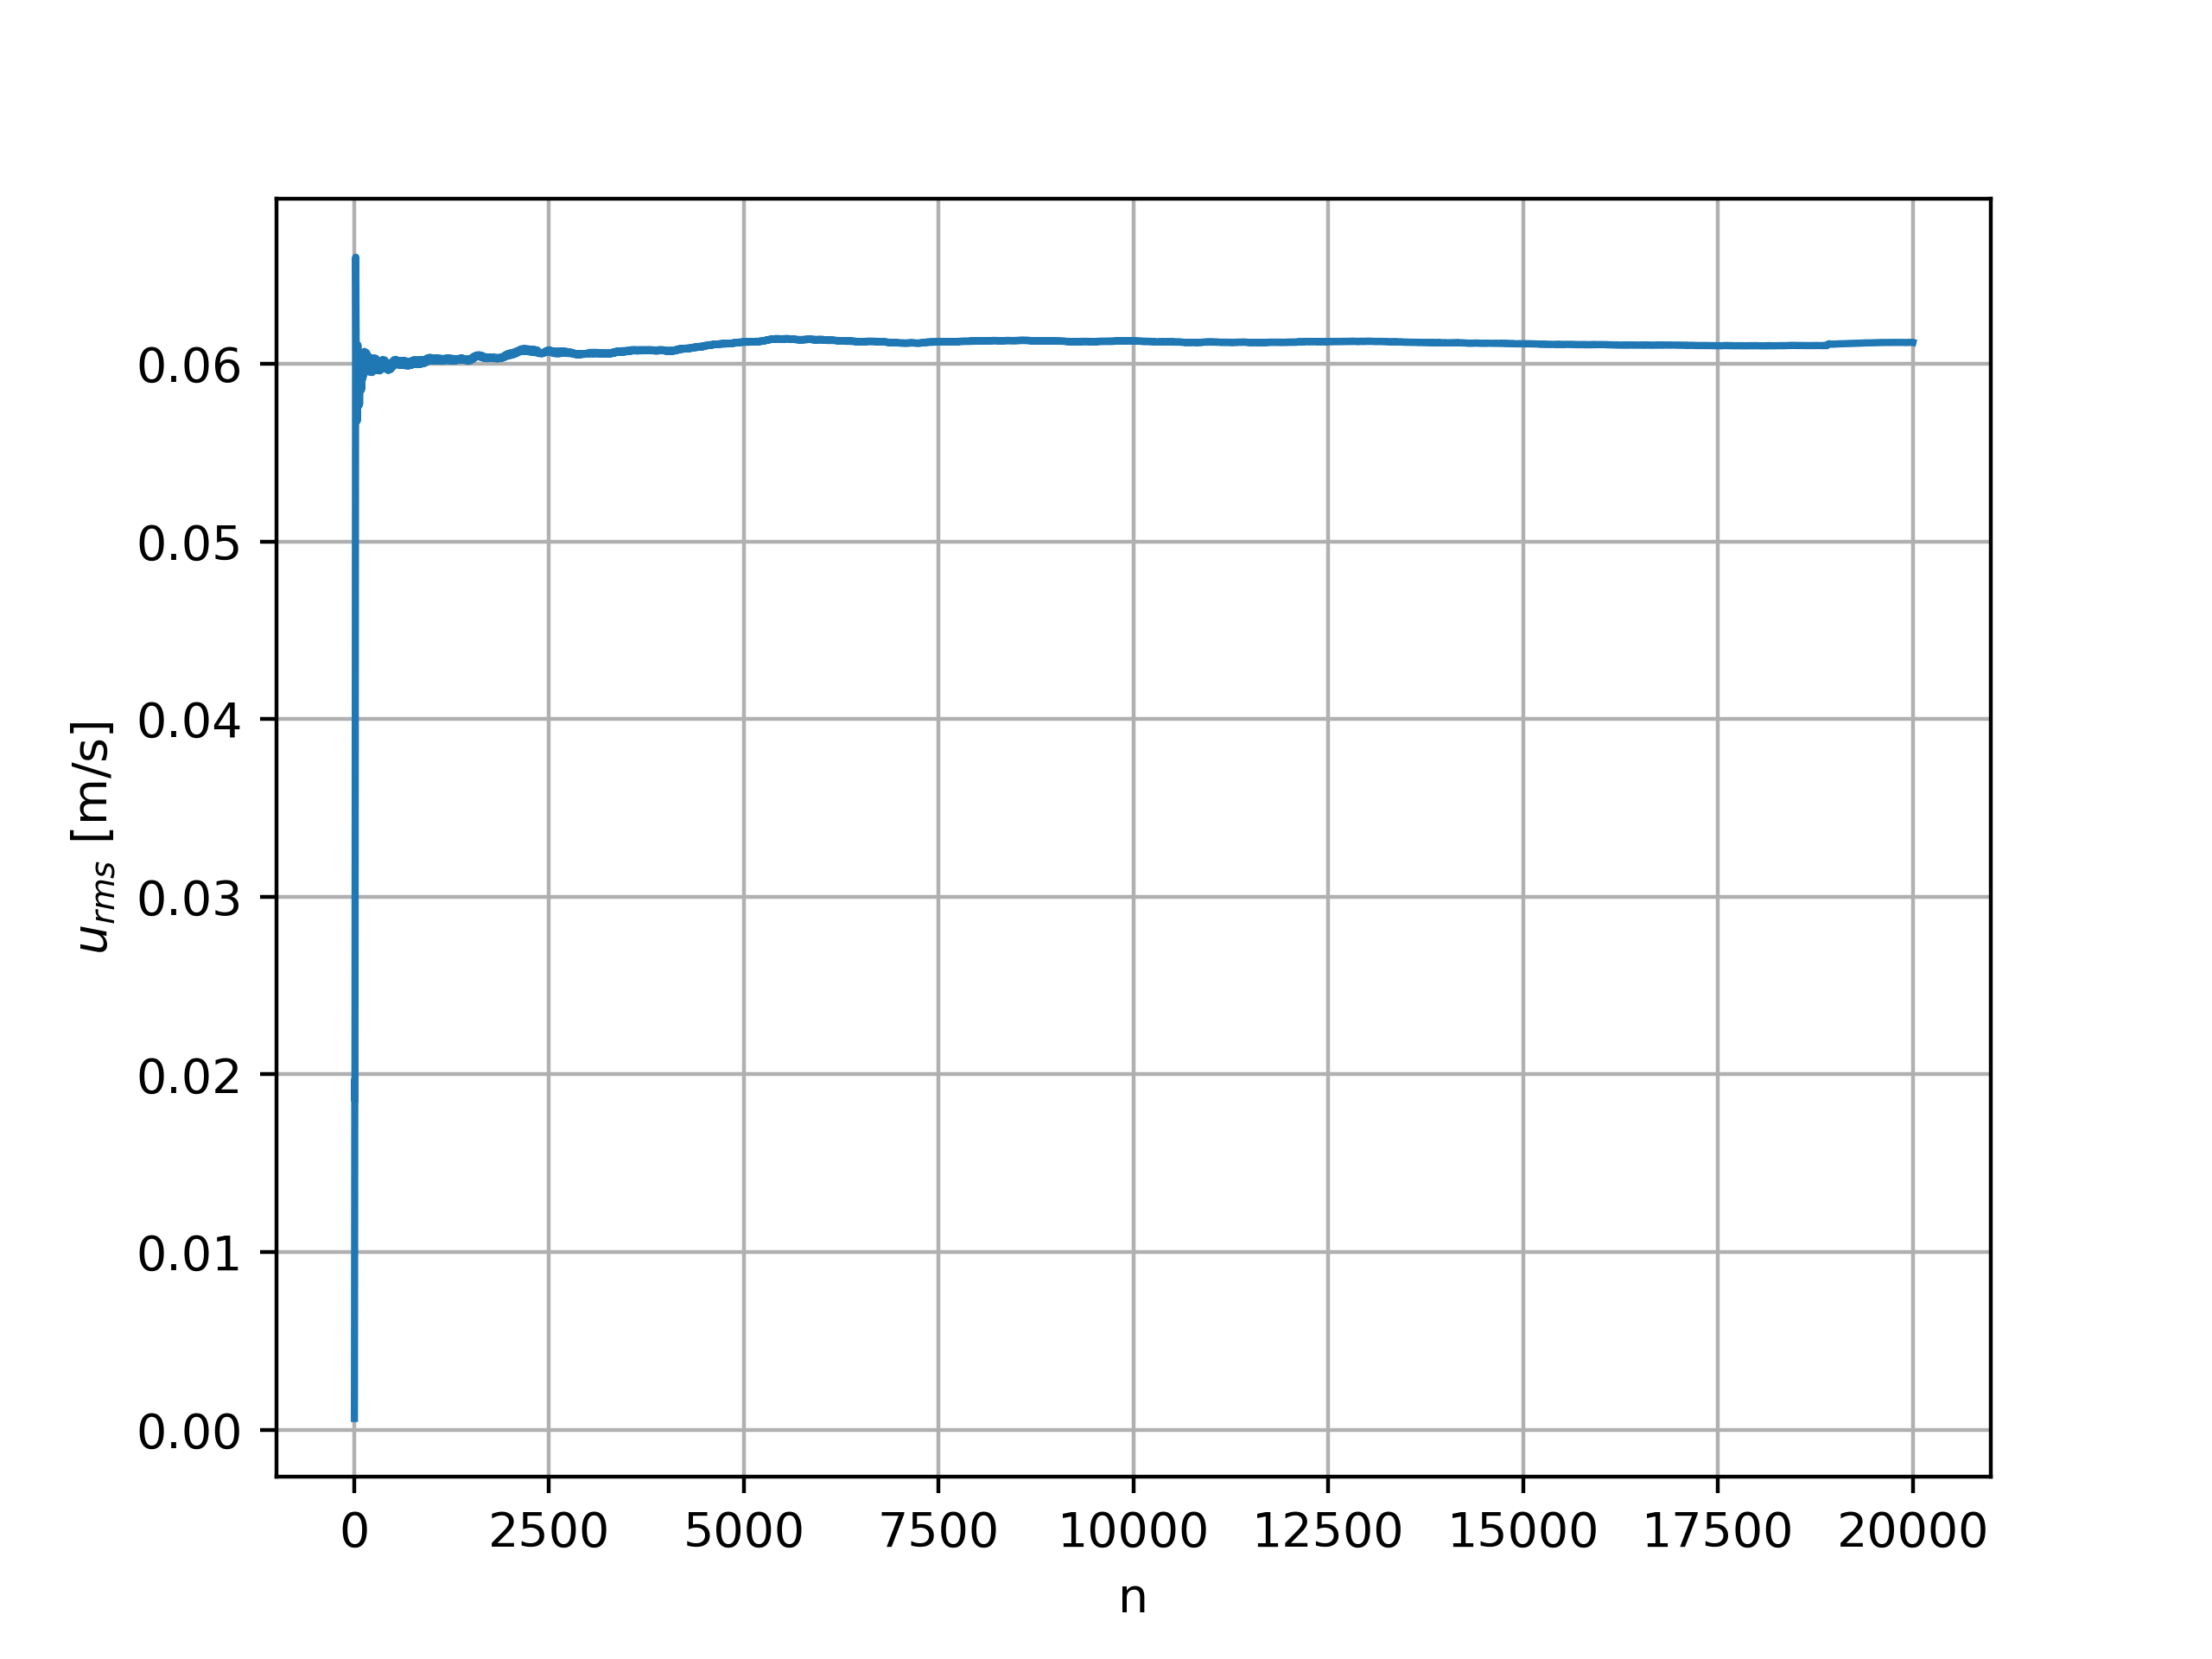
\includegraphics[width=.48\textwidth]{images/10/conv3.png}
    \caption{Analisi di convergenza della deviazione standard}
\end{figure}

\noindent Si osserva come i valori di velocità media e deviazione standard tendino ad un asintoto con l'aumentare del numero di punti considerati $n$.\\\\
Utilizzando delle grandezze adimensionali, rapportando la velocità media e la deviazione standard con il valore che assumono considerando tutti i 20000 punti, si ottiene il seguente diagramma:
\begin{figure}[H]
    \centering
    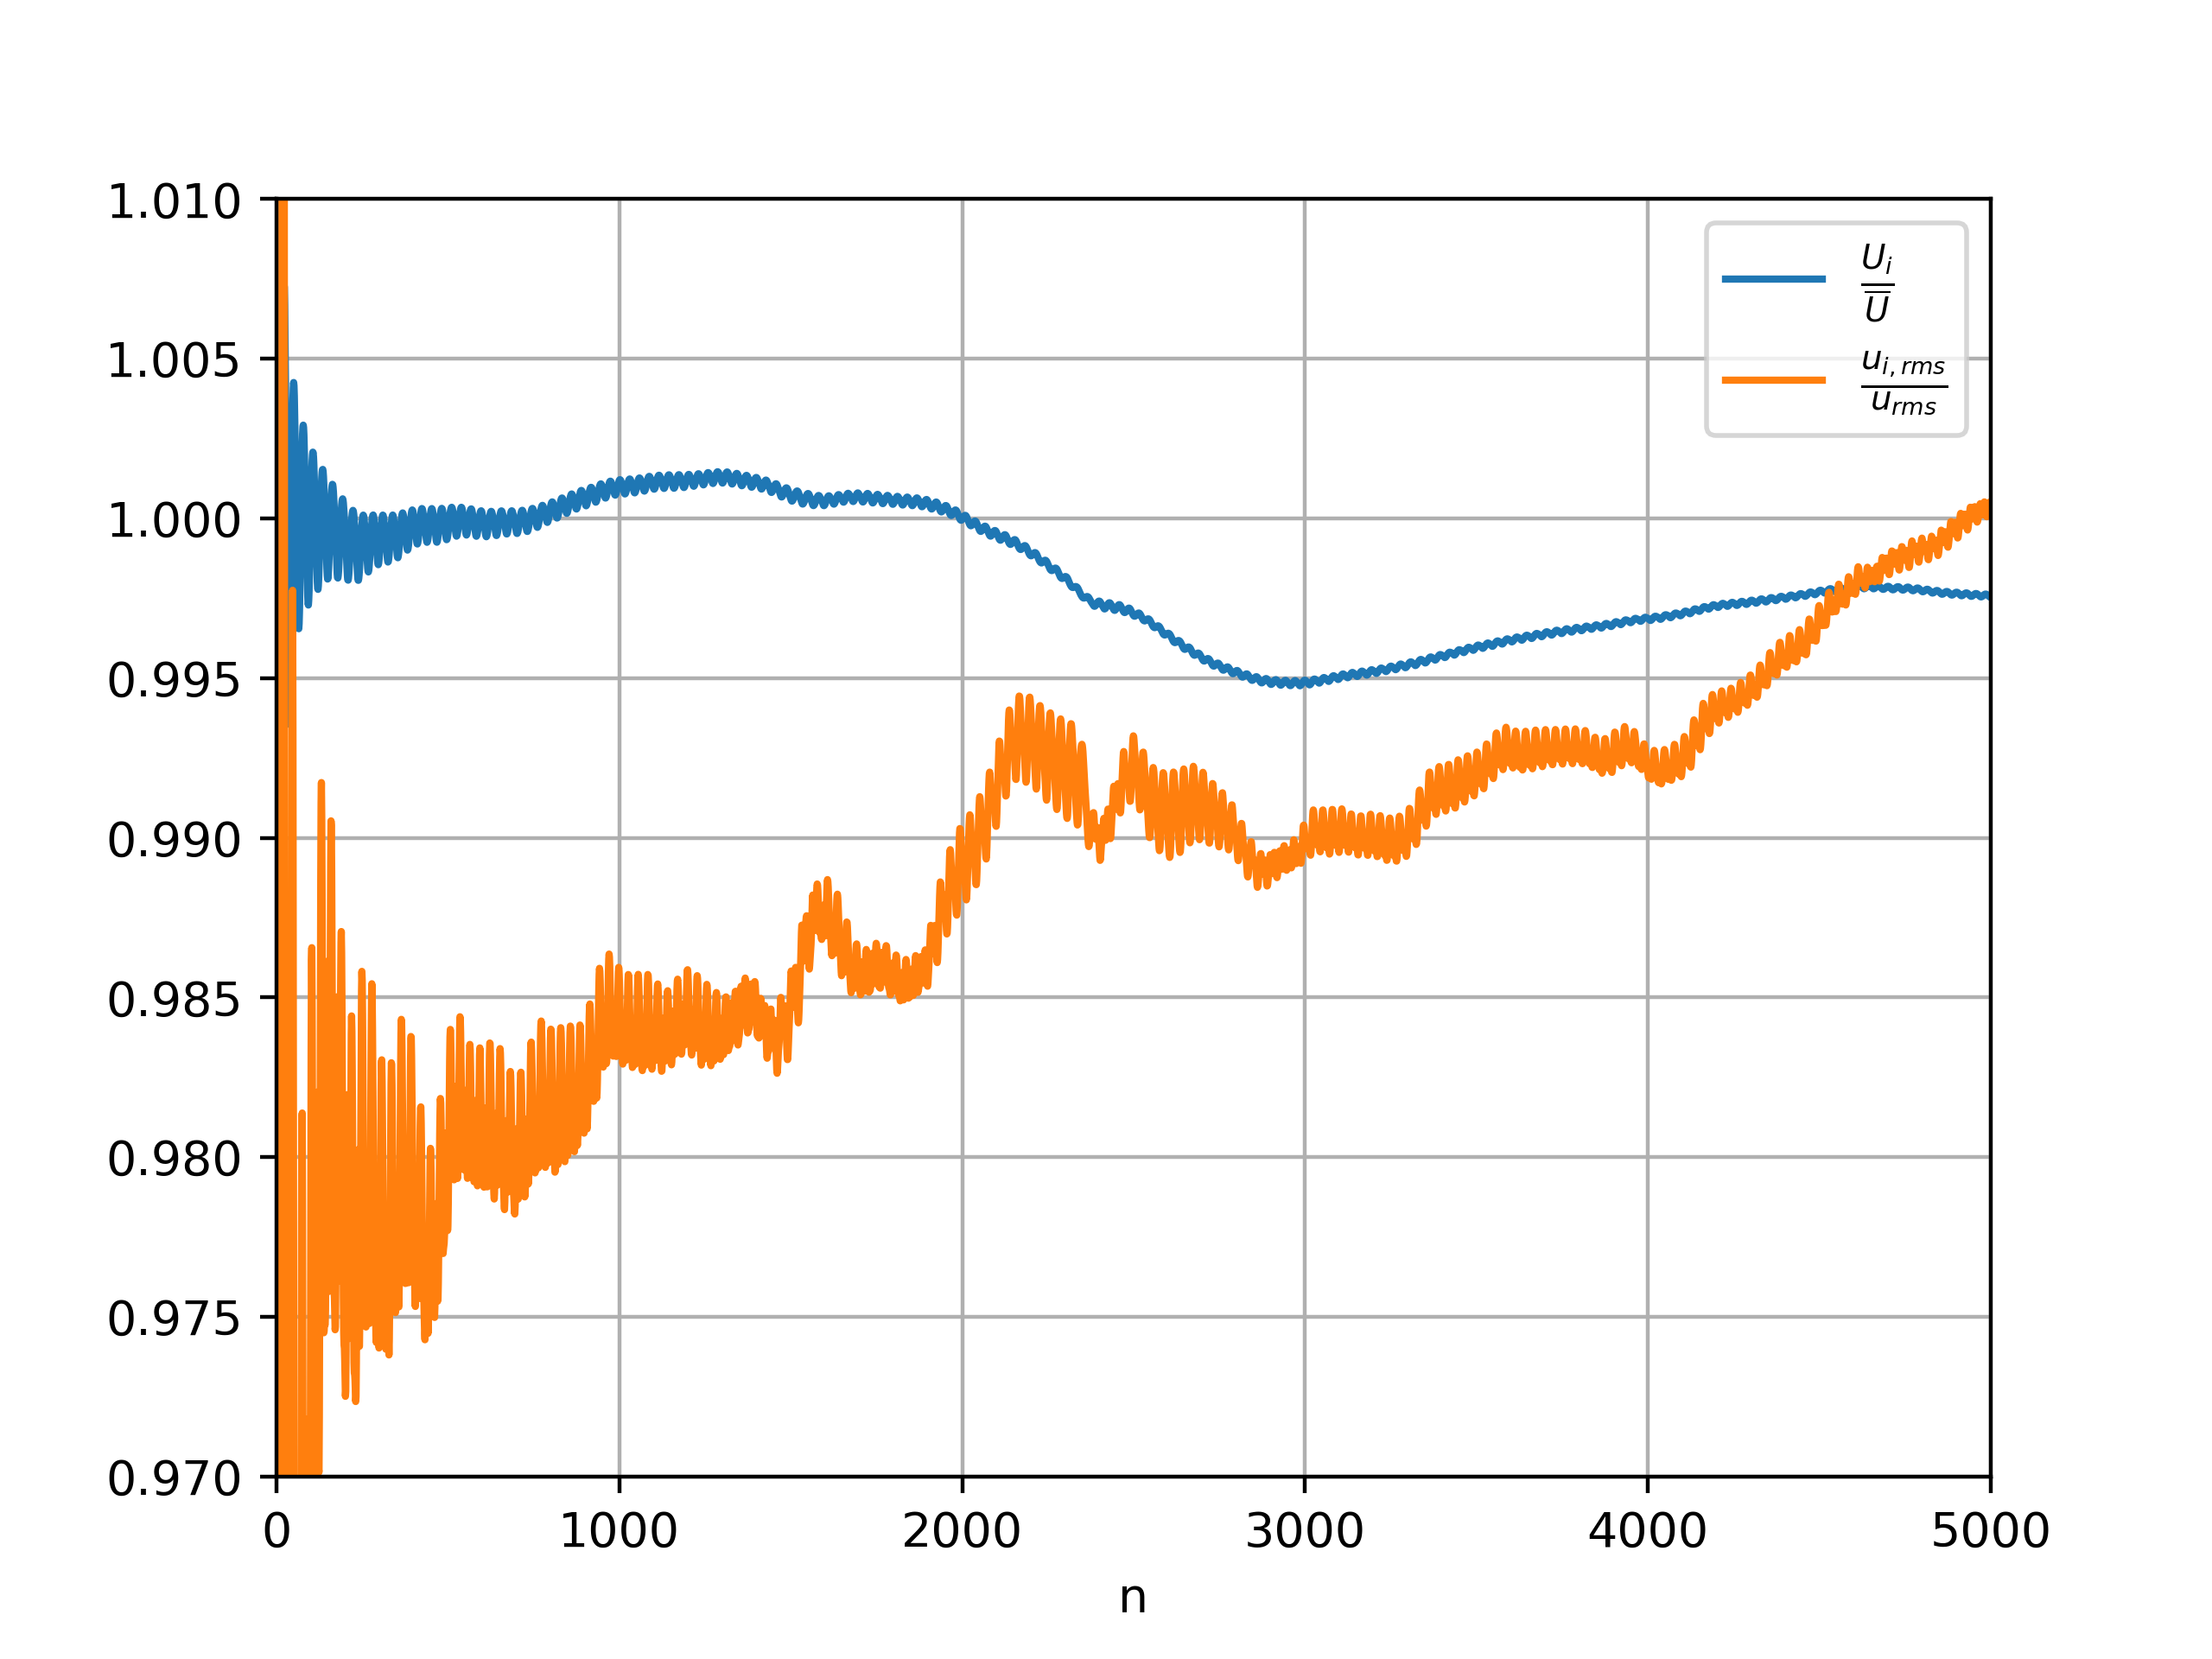
\includegraphics[width=.48\textwidth]{images/10/connvoverlapzoomed.png}
    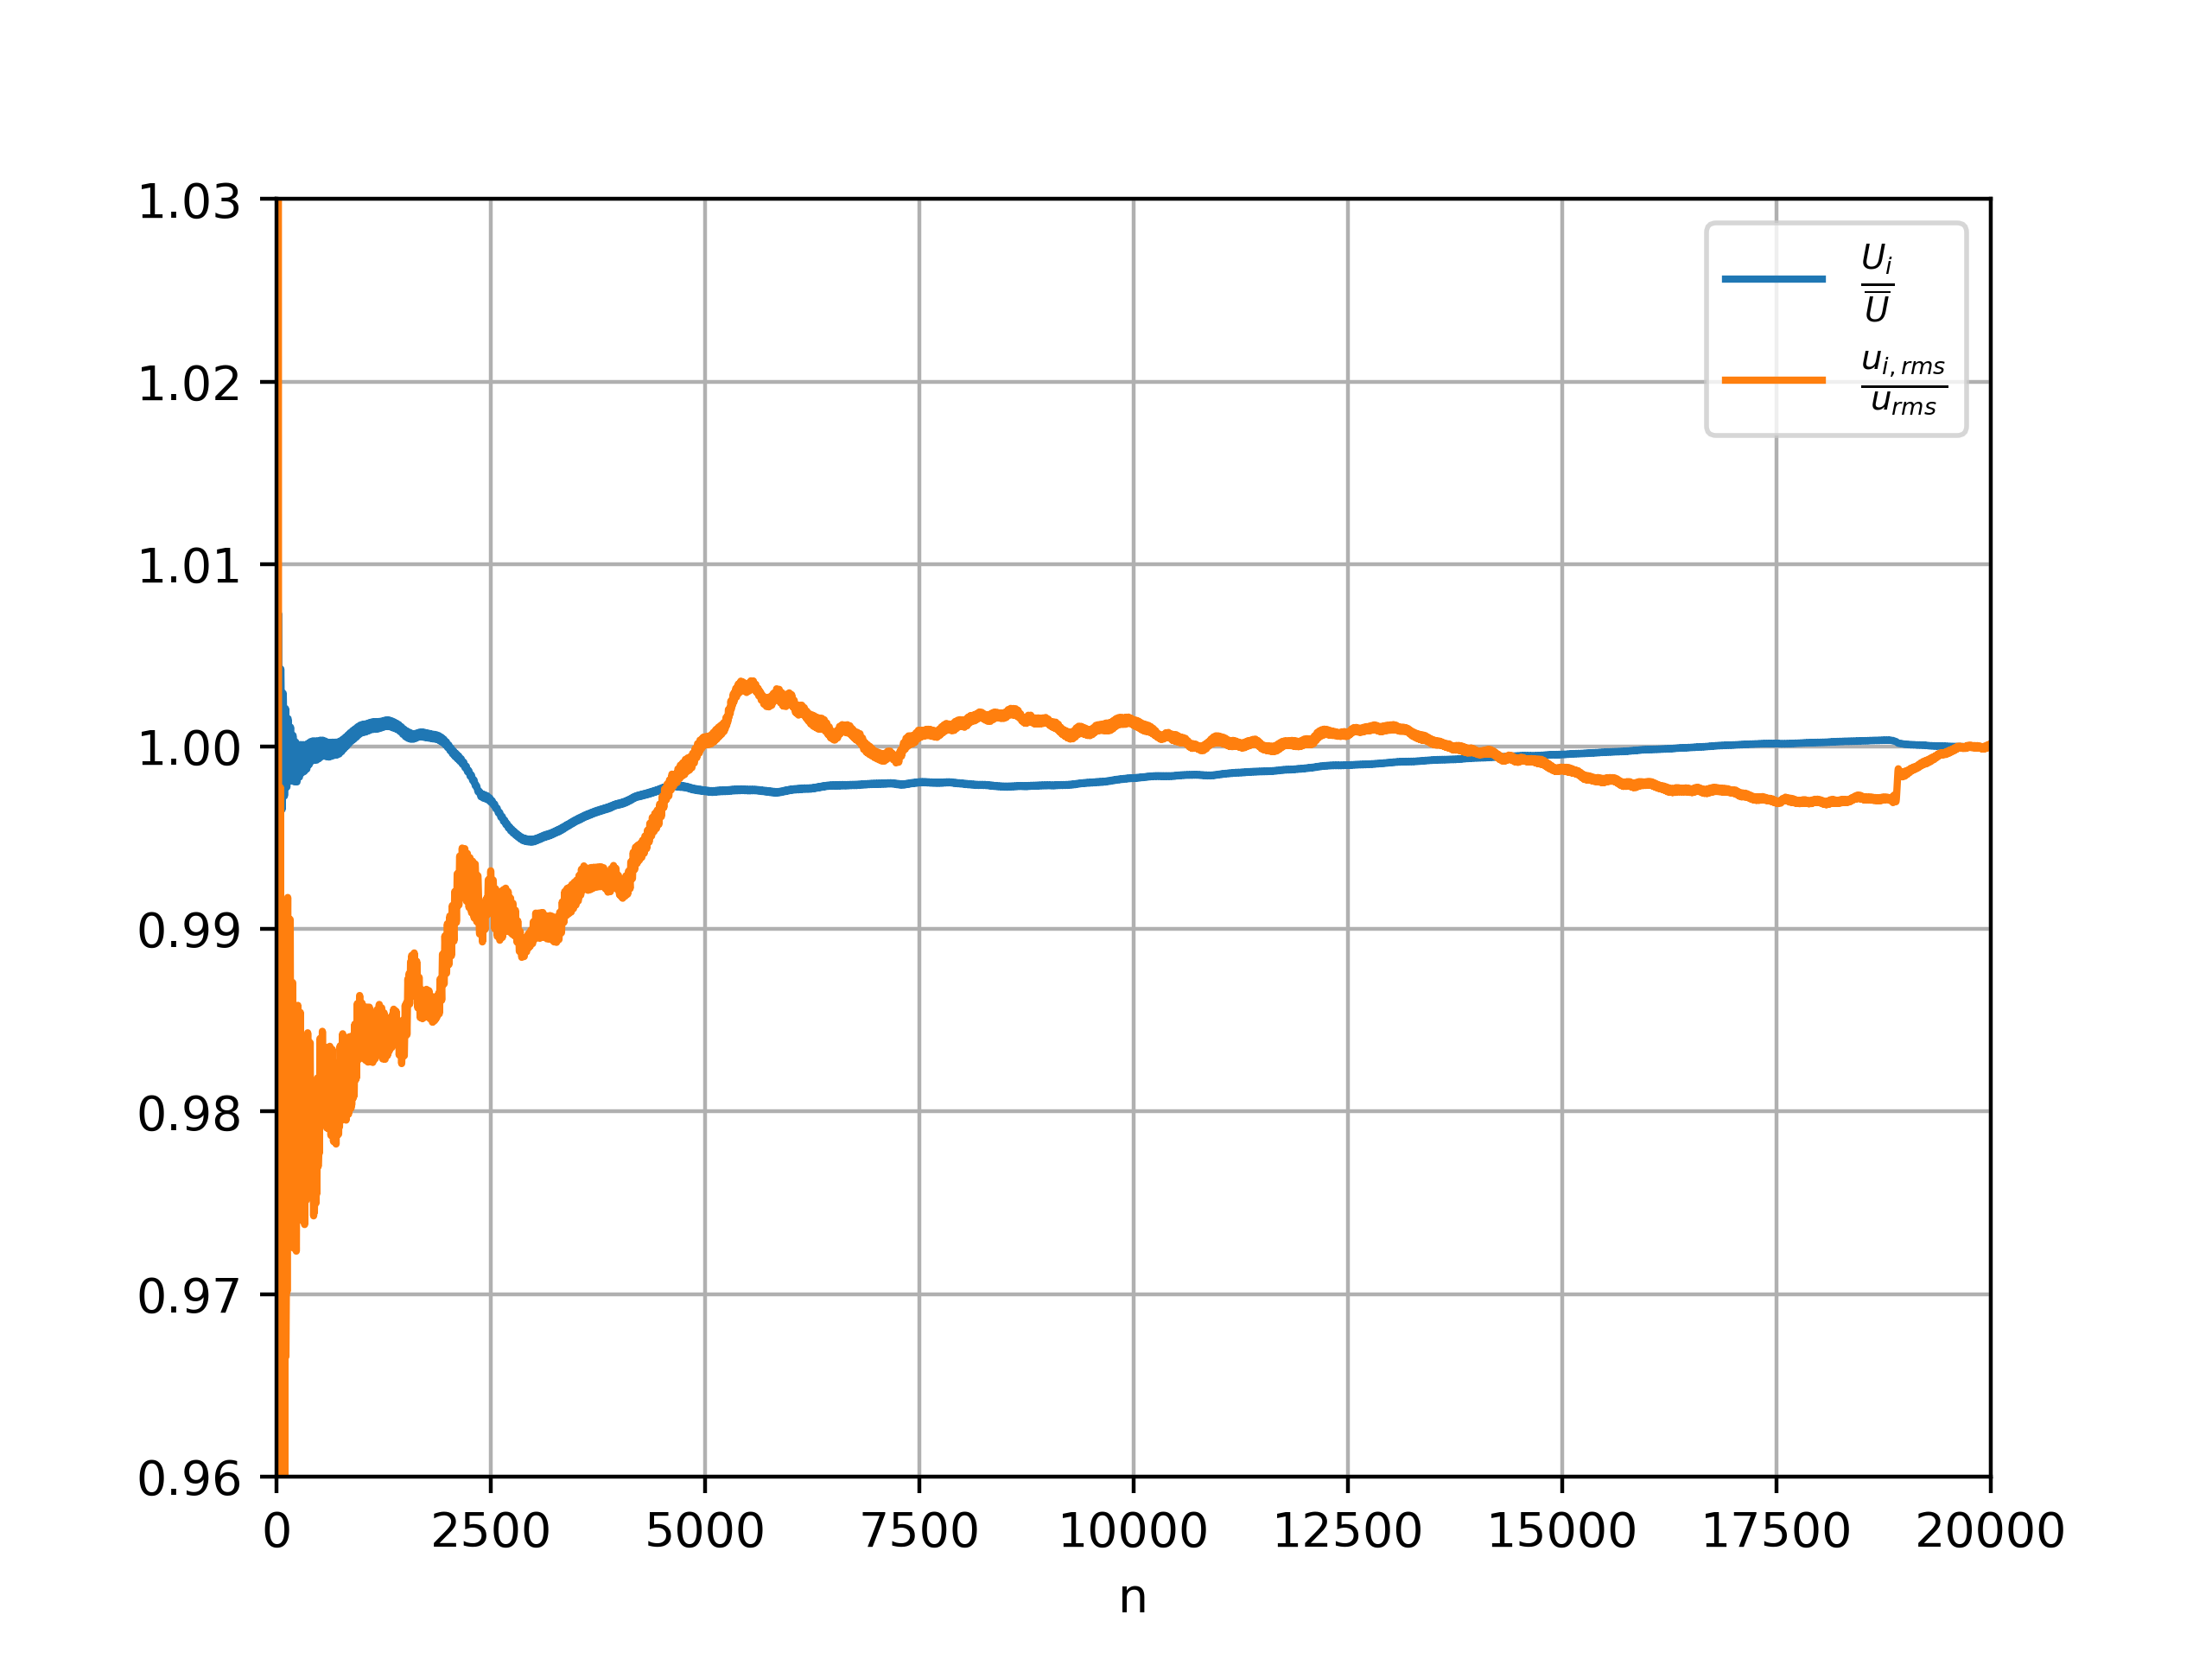
\includegraphics[width=.48\textwidth]{images/10/connvoverlap.png}
    \caption{Confronto tra velocità media e deviazione standard adimensionali}
\end{figure}

\noindent Si evince che la velocità media converge più velocemente (cioè con un numero di punti inferiore) rispetto alla deviazione standard.\\\\
Si può estendere l'analisi di convergenza ai momenti statistici di ordine superiore, considerando la skewness $S$ e la flatness $T$:
\begin{equation*}
    S = \frac{\overline{(U-\overline U)^3}}{u_{rms}^3} \qquad T = \frac{\overline{(U-\overline U)^4}}{u_{rms}^4}
\end{equation*}

\begin{figure}[H]
    \centering
    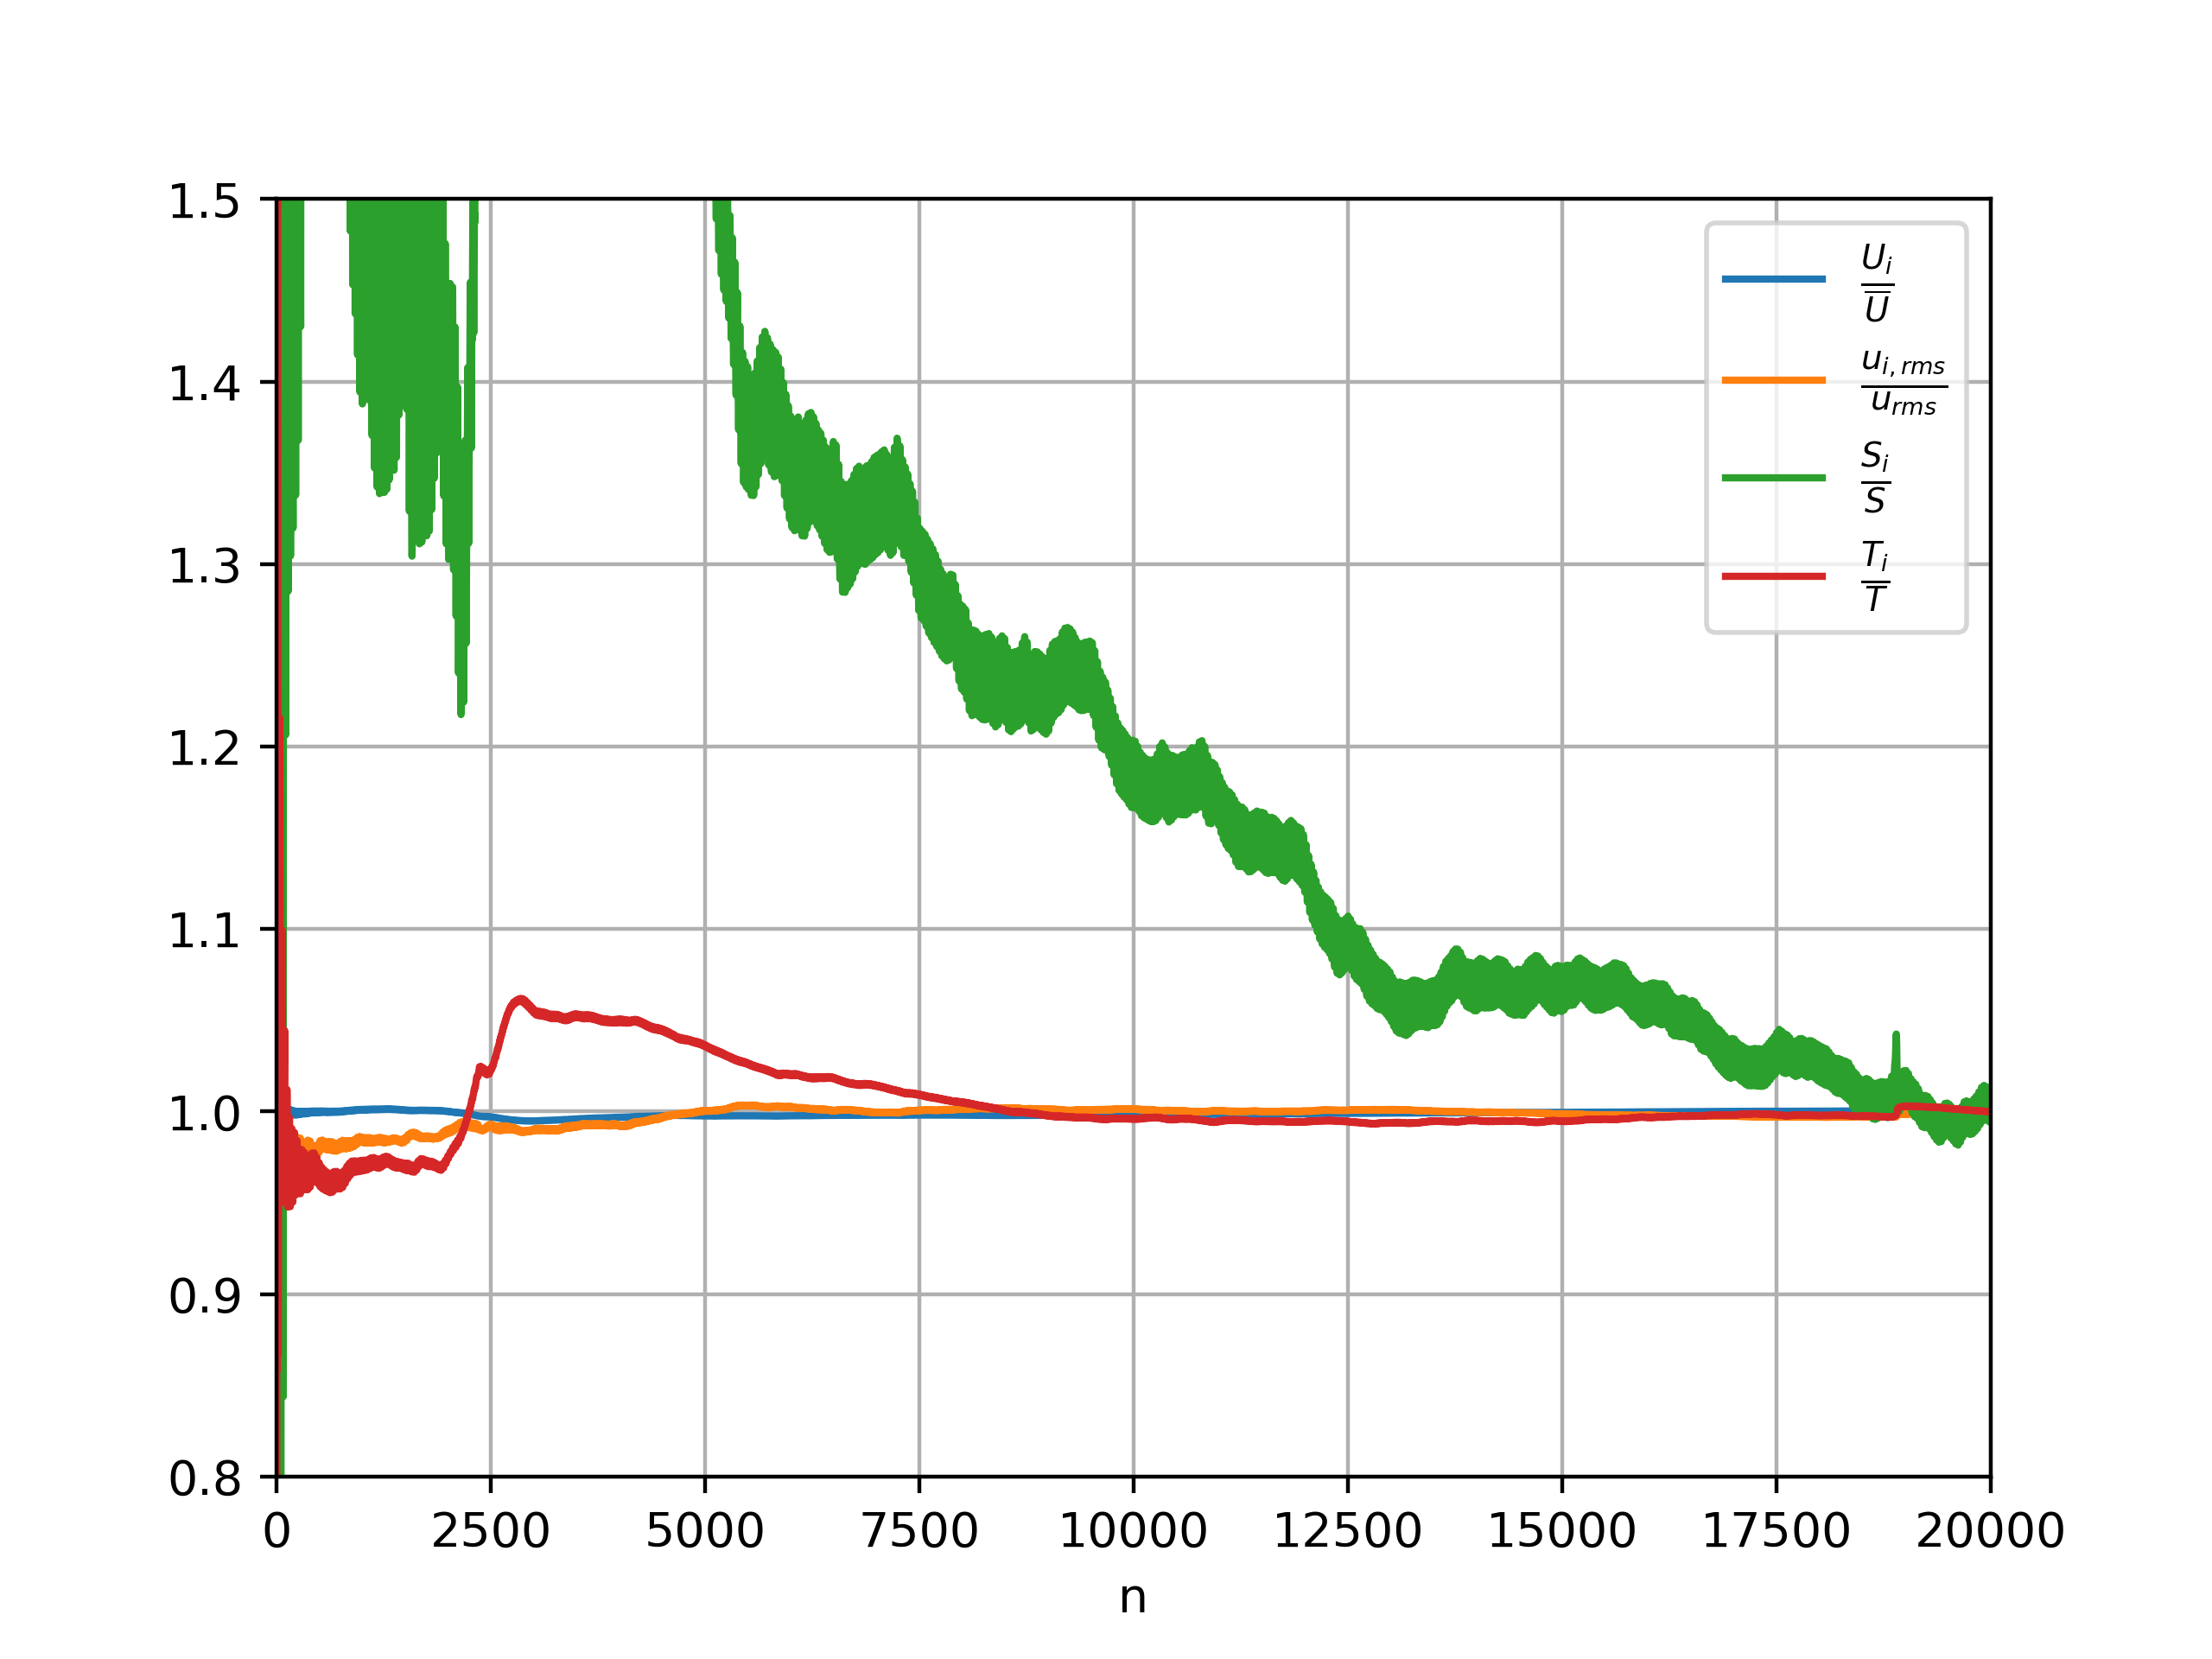
\includegraphics[width=.65\textwidth]{images/10/convall.png}
    \caption{Convergenza dei momenti statistici fino al quarto ordine}
\end{figure}

\noindent Si osserva come i momenti statistici di ordine superiore convergono più lentamente della velocità media e della deviazione standard.